%\documentclass[xcolor=dvipsnames,9pt]{beamer} 
%% 1. DUAL-DISPLAY NOTES:
%\documentclass[hyperref={bookmarks=false}]{beamer}
%\usepackage{pgfpages}
%\setbeameroption{show notes on second screen=left}

% 2. NOTES ON SEPARATE SLIDES:
%\documentclass[xcolor=dvipsnames,9pt,show notes]{beamer}

% 3. NOTES ONLY:
%\documentclass[xcolor=dvipsnames,9pt,show only notes]{beamer}

% 4. HANDOUTS:
%\documentclass[xcolor=dvipsnames,9pt,handout,show notes]{beamer}

% 5. NO NOTES: ONLY ONE THAT BUILDS WITHOUT WARNINGS
\documentclass[xcolor=dvipsnames,9pt,hide notes]{beamer}

%\setbeameroption{show only notes}
%\setbeameroption{show notes}

\usepackage{enumerate,amsmath,amssymb,fancyhdr,mathrsfs,amsthm,url,stmaryrd}
\usepackage{pgfpages}
\usepackage{listings}
%\usepackage{enumitem}

%% For creating a handout:
%\pgfpagesuselayout{4 on 1}[border shrink=5mm]
%\mode<handout>{\setbeamercolor{background canvas}{bg=black!5}}


\setbeamerfont{structure}{family=\rmfamily,shape=\scshape} 
\usepackage{graphicx}
\usepackage{tikz}
\usepackage{scalefnt}
\usetikzlibrary{matrix,arrows}

\usepackage{mathrsfs,textcomp}
\setbeamertemplate{navigation symbols}{}
\usepackage{verbatim}
\usepackage[mathcal]{euscript}

% This changes the color of alerted text to blue:
\definecolor{MyDarkBlue}{rgb}{0.2,0.2,0.7}
\definecolor{olivegreen}{cmyk}{0.64,0,0.95,0.40} % PANTONE 582
\setbeamercolor{alerted text}{fg=blue}
\newcommand{\emphcyan}[1]{\textcolor{MyDarkBlue}{\textbf{#1}}}
\renewcommand{\alert}[1]{\textcolor{MyDarkBlue}{\emph{#1}}}
\renewcommand{\alert}[1]{\textbf{{\emph{#1}}}}
% (default is red, but my slides are green and I don't like red and green together)

%\usecolortheme[named=OliveGreen]{structure} 
\usecolortheme[named=olivegreen]{structure} 
\setbeamertemplate{items}[ball] 
\setbeamertemplate{blocks}[rounded][shadow=true] 


% Commands for creating the ROTATING RECTANGLE
% Pass in a number which will be used to calculate the rotation angle.
% Example: Inside a tikzpicture environment, I would call 
%          \foreach \i in {0,...,11} { \eImageOfBZero{\i}  }
\newcommand{\eImageOfBZero}[1]{
  \pgfmathtruncatemacro{\r}{15*#1}
  \foreach \j in {1,2} {
    \draw[rotate around={\r:(-1,0.5)}] (\j -1, 0.5) node {$\j$};
    \pgfmathtruncatemacro{\x}{\j+3}
    \draw[rotate around={\r:(-1,0.5)}] (\j -1, -0.5) node {$\x$};
  }
  \draw[rotate around={\r:(-1,0.5)}] (-1, -0.5) node {$3$};
  \draw[rounded corners, dotted, rotate around={\r:(-1,0.5)}] (-1.5,-1) rectangle (1.5,1);
}

\newcommand{\eImageOfBOne}[1]{
  \pgfmathtruncatemacro{\r}{-15*#1}
  \foreach \j in {0,1,2} {
    \pgfmathtruncatemacro{\x}{10-\j}
    \draw[rotate around={\r:(-1,0.5)}] (\j -3, 1.5) node {$\x$};
  }
  \draw[rotate around={\r:(-1,0.5)}] (-3, .5) node {$7$} (-2, .5) node {$6$};
  \draw[rounded corners, dotted, rotate around={\r:(-1,0.5)}] (-3.5,0) rectangle (-0.5,2);
}

\newcommand{\eImageOfBTwo}[1]{
  \pgfmathtruncatemacro{\r}{15*#1}
  \foreach \j in {0,1,2} {
    \pgfmathtruncatemacro{\x}{15-\j}
    \draw[rotate around={\r:(1,0.5)}] (\j+1,1.5) node {$\x$};
  }
  \draw[rotate around={\r:(1,0.5)}] (3, .5) node {$11$} (2, .5) node {$12$};
  \draw[rounded corners, dotted,rotate around={\r:(1,0.5)}] (3.5,0) rectangle (0.5,2);
}

%%%% INSERT MACROS %%%%

\newcommand{\PUTIN}{{\text {\bf **********PUT IN**********}}}



%\newcommand{\typo}[1]{{\color{red} #1}}
\newcommand{\typo}[1]{{#1}}

\DeclareMathOperator{\dom}{dom}

\newcommand{\todo}[1]{
\ifthenelse{\boolean{todos}}{~\\{\bf TODO(wjd):} \emph{#1}\\}{}
}

% names
\newcommand{\Jiri}{Ji\v{r}\'i}
\newcommand{\Tuma}{T\r{u}ma}
\newcommand{\Palfy}{P\'alfy}
\newcommand{\Pudlak}{Pudl\'ak}
\newcommand{\PP}{P\'alfy-Pudl\'ak}
\newcommand{\PhP}{P\'alfy-Pudl\'ak}
\newcommand{\PAP}{P\'alfy\ and Pudl\'ak}
\newcommand{\Gratzer}{Gr\"{a}tzer}
\newcommand{\<}{\ensuremath{\langle}}
\renewcommand{\>}{\ensuremath{\rangle}}
\newcommand{\beps}{\ensuremath{\boldsymbol{\varepsilon}}}

% SET THEORY & RELATIONS
% To specifiy that the symbol R is a binary relation use: x \rel{R} y
\newcommand{\rel}[1]{\ensuremath{\mathbin{#1}}}
\newcommand{\rR}{\ensuremath{\rel{R}}}  % or just x \rR y
\newcommand{\fld}{\ensuremath{\mathrm{fld}\,}}   % the field of a relation
\newcommand{\ran}{\ensuremath{\mathrm{ran}\,}}   % the range of a relation
\newcommand{\card}{\ensuremath{\mathrm{card}\,}} % cardinality
\newcommand{\res}{\ensuremath{\upharpoonright}}  % restriction
\newcommand{\es}{\ensuremath{\emptyset}}
\newcommand{\lb}{\ensuremath{\llbracket}}
\newcommand{\rb}{\ensuremath{\rrbracket}}
\newcommand{\arity}{\ensuremath{\mathfrak{a}}}
\newcommand{\ar}{\ensuremath{\mathrm{ar}}}

% binary operations
%% \newcommand{\subnormal}{\ensuremath{\trianglelefteqslant}}
%% \newcommand{\supnormal}{\ensuremath{\trianglerighteqslant}}
%% \newcommand{\notsubnormal}{\ensuremath{\ntrianglelefteqslant}}
\renewcommand{\leq}{\ensuremath{\leqslant}}
\renewcommand{\nleq}{\ensuremath{\nleqslant}}
\renewcommand{\geq}{\ensuremath{\geqslant}}
%\renewcommand{\lneq}{\ensuremath{\lneqslant}}
\renewcommand{\gneq}{\ensuremath{\gneqslant}}
\renewcommand{\ngeq}{\ensuremath{\ngeqslant}}
\newcommand{\ssubnormal}{\ensuremath{\vartriangleleft}}
\newcommand{\subnormal}{\ensuremath{\trianglelefteqslant}}
\newcommand{\supnormal}{\ensuremath{\trianglerighteqslant}}
\newcommand{\notsubnormal}{\ensuremath{\ntrianglelefteqslant}}
\newcommand{\meet}{\ensuremath{\wedge}}
\newcommand{\join}{\ensuremath{\vee}}
\newcommand{\Meet}{\ensuremath{\bigwedge}}
\renewcommand{\Join}{\ensuremath{\bigvee}}

% ALGEBRAS

% fields
\newcommand{\F}{\ensuremath{\mathbb{F}}}   % arbitrary field
\newcommand{\Z}{\ensuremath{\mathbb{Z}}}   % integers
\newcommand{\Q}{\ensuremath{\mathbb{Q}}}   % rational numbers
\newcommand{\N}{\ensuremath{\mathbb{N}}}   % natural numbers

\newcommand{\Hom}{\ensuremath{\mathrm{Hom}}}
\newcommand{\HomR}{\ensuremath{\mathrm{Hom}_R}}
\newcommand{\End}{\ensuremath{\mathrm{End}}}
\newcommand{\Aut}{\ensuremath{\mathrm{Aut}}}

\newcommand{\ID}[1]{\ensuremath{\mathcal{ID}(#1)}}
%\newcommand{\idemdec}{\ensuremath{\mbox{Idemdec}(X)}}
\newcommand{\idemdec}{\ID{X}}
\newcommand{\EqX}{\ensuremath{\mbox{Eq}(X)}}
\newcommand{\Eq}{\ensuremath{\mathrm{Eq}}}
\newcommand{\bEq}{\ensuremath{\mathbf{Eq}}}
\newcommand{\bEqX}{\ensuremath{\mathbf{Eq}(X)}}
\newcommand{\Cg}{\ensuremath{\mathrm{Cg}}}
\newcommand{\Sg}{\ensuremath{\mathrm{Sg}}}
\newcommand{\Stab}{\ensuremath{\mathrm{Stab}}}
\newcommand{\bCon}{\ensuremath{\mathbf{Con\,}}}
\newcommand{\Con}{\ensuremath{\mathrm{Con\,}}}
\newcommand{\Sub}{\ensuremath{\mathrm{Sub}}}
\newcommand{\CSub}{\ensuremath{\mathrm{CSub\,}}}
\newcommand{\Pol}{\ensuremath{\mathrm{Pol}}}
\newcommand{\Clo}{\ensuremath{\mathrm{Clo}}}
%\newcommand{\Pol1}{\ensuremath{\mathrm{Pol}_1}}
\newcommand{\Sym}{\ensuremath{\mathrm{Sym}}}
\newcommand{\core}{\ensuremath{\mathrm{core}}}

\newcommand{\ps}[1]{\ensuremath{^{(#1)}}}
\newcommand{\piB}{\ensuremath{\pi_B}}
\newcommand{\hpsi}{\ensuremath{\hat{\psi}}}
\newcommand{\htheta}{\ensuremath{\hat{\theta}}}
%\newcommand{\supi}{\ensuremath{^{(i)}}}
\newcommand{\supi}{\ensuremath{^{i}}}
%\newcommand{\supj}{\ensuremath{^{(j)}}}
\newcommand{\supj}{\ensuremath{^{j}}}

\newcommand{\FLRP}{{\small FLRP}}
\newcommand{\flrp}{{\small FLRP}}

% SOFTWARE
\newcommand{\GAP}{\textsf{GAP}}
\newcommand{\gap}{\textsf{GAP}}
\newcommand{\XGAP}{\textsf{XGAP}}
\newcommand{\xgap}{\textsf{XGAP}}
\newcommand{\uacalc}{\textsf{UACalc}}
\newcommand{\codesize}{\footnotesize}

\newcommand{\tensor}{\ensuremath{\otimes}}

% \newcommand{\ex}{\marginpar[{\LARGE \Bicycle}]{{\LARGE \Bicycle}}}
\newcommand{\leftsubR}{\ensuremath{ { _R }}}
\newcommand{\power}[1]{\ensuremath{\mathscr{P}(#1)}}
\newcommand{\0}{\ensuremath{\mathbf{0}}}
\newcommand{\1}{\ensuremath{\mathbf{1}}}
\newcommand{\2}{\ensuremath{\mathbf{2}}}
\newcommand{\3}{\ensuremath{\mathbf{3}}}
\newcommand{\4}{\ensuremath{\mathbf{4}}}
\newcommand{\5}{\ensuremath{\mathbf{5}}}

\newcommand{\bA}{\ensuremath{\mathbf{A}}}
\newcommand{\cA}{\ensuremath{\mathcal{A}}}
\newcommand{\fA}{\ensuremath{\mathfrak{A}}}
\newcommand{\sA}{\ensuremath{\mathscr{A}}}

\newcommand{\cB}{\ensuremath{\mathcal{B}}}
\newcommand{\bB}{\ensuremath{\mathbf{B}}}
\newcommand{\bBi}{\ensuremath{\mathbf{B}_i}}
\newcommand{\sB}{\ensuremath{\mathscr{B}}}
\newcommand{\fB}{\ensuremath{\mathfrak{B}}}

\newcommand{\bC}{\ensuremath{\mathbf{C}}}
\newcommand{\cC}{\ensuremath{\mathcal{C}}}
\newcommand{\fC}{\ensuremath{\mathfrak{C}}}
\newcommand{\sC}{\ensuremath{\mathscr{C}}}

\newcommand{\bd}{\ensuremath{\mathbf{d}}}

\newcommand{\bE}{\ensuremath{\mathbf{E}}}
\newcommand{\sE}{\ensuremath{\mathscr{E}}}

\newcommand{\bF}{\ensuremath{\mathbf{F}}}
\newcommand{\sF}{\ensuremath{\mathscr{F}}}

\newcommand{\bG}{\ensuremath{\mathbf{G}}}
\newcommand{\sG}{\ensuremath{\mathscr{G}}}
\newcommand{\barG}{\ensuremath{\overline{G}}}
\newcommand{\barg}{\ensuremath{\overline{g}}}
\newcommand{\G}{\ensuremath{\mathfrak{G}}}

\newcommand{\bH}{\ensuremath{\mathbf{H}}}
\newcommand{\sH}{\ensuremath{\mathscr{H}}}
\newcommand{\barH}{\ensuremath{\overline{H}}}
\newcommand{\barh}{\ensuremath{\overline{h}}}

\newcommand{\cI}{\ensuremath{\mathcal{I}}}
\newcommand{\sI}{\ensuremath{\mathscr{I}}}
\newcommand{\fI}{\ensuremath{\mathfrak{I}}}

\newcommand{\cJ}{\ensuremath{\mathcal{J}}}
\newcommand{\sJ}{\ensuremath{\mathscr{J}}}
\newcommand{\fJ}{\ensuremath{\mathfrak{J}}}

\newcommand{\sK}{\ensuremath{\mathscr{K}}}

\newcommand{\bL}{\ensuremath{\mathbf{L}}}
\newcommand{\sL}{\ensuremath{\mathscr{L}}}

\newcommand{\M}{\ensuremath{\mathbb{M}}}
\newcommand{\bM}{\ensuremath{\mathbf{M}}}
\newcommand{\bN}{\ensuremath{\mathbf{N}}}
\newcommand{\bn}{\ensuremath{\mathbf{n}}}

\newcommand{\bO}{\ensuremath{\mathbf{O}}}
\newcommand{\sO}{\ensuremath{\mathscr{O}}}
\newcommand{\cO}{\ensuremath{\mathcal{O}}}

\newcommand{\bOmega}{\ensuremath{\alg \Omega}}
\newcommand{\ConO}{\ensuremath{\Con \bOmega}}

\newcommand{\bP}{\ensuremath{\mathbf{P}}}
\newcommand{\sP}{\ensuremath{\mathscr{P}}}
\newcommand{\cP}{\ensuremath{\mathcal{P}}}

\newcommand{\bR}{\ensuremath{\mathbf{R}}}

\newcommand{\sS}{\ensuremath{\mathscr{S}}}
\newcommand{\bS}{\ensuremath{\mathbf{S}}}
\newcommand{\bs}{\ensuremath{\mathbf{s}}}
\newcommand{\sT}{\ensuremath{\mathscr{T}}}

\newcommand{\V}{\ensuremath{\mathrm{V}}}
\newcommand{\sV}{\ensuremath{\mathscr{V}}}

\newcommand{\bX}{\ensuremath{\mathbf{X}}}
\newcommand{\bx}{\ensuremath{\mathbf{x}}}
\newcommand{\barx}{\ensuremath{\overline{x}}}

\newcommand{\bY}{\ensuremath{\mathbf{Y}}}
\newcommand{\by}{\ensuremath{\mathbf{y}}}
\newcommand{\bary}{\ensuremath{\overline{y}}}

% miscellaneous
\newcommand{\dotsize}{.8pt}
\newcommand{\giant}{\ensuremath{\mathfrak{Gi}}}
\newcommand{\solvable}{\ensuremath{\mathfrak{S}}}
\newcommand{\si}{\ensuremath{\mathfrak{SI}}}
\renewcommand{\iff}{\ensuremath{\quad \Leftrightarrow \quad}}
\newcommand{\ISLE}{{\small ISLE}}
\newcommand{\Soc}{\ensuremath{\mathrm{Soc}}}
\newcommand{\AGL}{\ensuremath{\mathrm{AGL}}}
\newcommand{\Out}{\ensuremath{\mathrm{Out}}}
\newcommand{\Inn}{\ensuremath{\mathrm{Inn}}}
\newcommand{\stab}[1]{\ensuremath{G_{#1}}}
\newcommand{\Gset}{\ensuremath{G\text{-set}}}
\newcommand{\Gsets}{\ensuremath{G\text{-sets}}}
\newcommand{\Mset}{\ensuremath{M\text{-set}}}
\newcommand{\con}[1]{\op{Con}\;\alg #1}	%% Con A  as a set
%\newcommand{\Con}[1]{\alg{Con}\;\alg #1}	%% Con A  as an lattice
\newcommand{\iso}{\DOTSB\cong}			%% isomorphism
\newcommand{\cov}{\prec}		%% a cover sign
\newcommand{\covs}{\succ}		%% the reverse, "a covers b" sign
\newcommand{\ConA}{\ensuremath{\mathbf{Con}(\mathbf{A})}}
\newcommand{\op}{\operatorname}			%% Should be used for J(w) etc.
\newcommand{\alg}[1]{\mathbf{#1}}
\newcommand{\la}{\langle}	     %% left angle for order sequences <a,b>
\newcommand{\ra}{\rangle}	     %% right angle
\newcommand{\id}{\ensuremath{\mathrm{id}}}
\renewcommand{\phi}{\ensuremath{\varphi}}
\newcommand{\bphi}{\ensuremath{\bar{\varphi}}}
\newcommand{\ann}{\ensuremath{\mathrm{ann}}}
\newcommand{\Tor}{\ensuremath{\mathrm{Tor}}}
\newcommand{\image}{\ensuremath{\mathrm{im}}}
\newcommand{\im}{\ensuremath{\mathrm{im}}}
\newcommand{\Tr}{\ensuremath{\mathrm{Tr}}}
\newcommand{\upalpha}{\ensuremath{\alpha^{\uparrow}}}
\newcommand{\downalpha}{\ensuremath{\alpha^{\downarrow}}}
\newcommand{\upbeta}{\ensuremath{\beta^{\uparrow}}}
\newcommand{\downbeta}{\ensuremath{\beta^{\downarrow}}}
\newcommand{\resB}{\ensuremath{|_{_B}}}
\newcommand{\resBi}{\ensuremath{|_{_{B_i}}}}
\newcommand{\eps}{\ensuremath{\varepsilon}}
\newcommand{\hatmap}{\ensuremath{\widehat{\phantom{x}}}}
\newcommand{\one}{\ensuremath{\mathbf{1}}}
\newcommand{\two}{\ensuremath{\mathbf{2}}}
\newcommand{\three}{\ensuremath{\mathbf{3}}}
\newcommand{\tbeta}{\ensuremath{\widetilde{\beta}}}
\newcommand{\hbeta}{\ensuremath{\widehat{\beta}}}
\newcommand{\cick}{\ensuremath{\sC_i}}
\newcommand{\CE}{\ensuremath{\sC_i^{\sE}}}
\newcommand{\CO}{\ensuremath{\sC_i^{\sO}}}
\newcommand{\CICK}{\ensuremath{c_i/\beta \cup c^{K+1}_i/\beta^{\bB_{K+1}}}}
\newcommand{\GL}{\ensuremath{\mathrm{GL}}}
\newcommand{\PSL}{\ensuremath{\mathrm{PSL}}}



\renewcommand{\phi}{\ensuremath{\varphi}}
\newcommand{\Hawaii}{Hawai\kern.05em`\kern.05em\relax i}
\newcommand{\Manoa}{M\=anoa}
%% \newcommand{\GAP}{{\small GAP}}
%% \newcommand{\cd}{\ensuremath{\otimes}}
%% \newcommand{\con}[1]{\ensuremath{\langle #1 \rangle}}
%% \newcommand{\ii}[1]{{\it #1}}
%% \newcommand{\power}[1]{\ensuremath{\mathscr{P}(#1)}}
%% \newcommand{\scrA}{\ensuremath{\mathscr{A}}}
%% \newcommand{\bM}{\ensuremath{\mathbf{M}}}
%% \newcommand{\Mn}{\ensuremath{\mathbf{M}_n}}
%% \newcommand{\bF}{\ensuremath{\mathbf{F}}}
%% \newcommand{\bE}{\ensuremath{\mathbf{E}}}
%% \newcommand{\bR}{\ensuremath{\mathbf{R}}}
%% \newcommand{\bA}{\ensuremath{\mathbf{A}}}
%% \newcommand{\bG}{\ensuremath{\mathbf{G}}}
%% \newcommand{\bH}{\ensuremath{\mathbf{H}}}
%% \newcommand{\bK}{\ensuremath{\mathbf{K}}}
%% \newcommand{\bL}{\ensuremath{\mathbf{L}}}
%% \newcommand{\bB}{\ensuremath{\mathbf{B}}}
%% \newcommand{\svert}{\ensuremath{\; \vert \; }}
%% \newcommand{\Z}{\ensuremath{\mathbb{Z}}}
%% \newcommand{\sE}{\ensuremath{\mathcal{E}}}
%% \newcommand{\sO}{\ensuremath{\mathcal{O}}}
%% \newcommand{\sH}{\ensuremath{\mathcal{H}}}
%% \newcommand{\sS}{\ensuremath{\mathcal{S}}}
%% %\newcommand{\sL}{\ensuremath{\mathcal{L}}}
%% \newcommand{\sL}{\ensuremath{\mathscr{L}}}
%% \newcommand{\bN}{\ensuremath{\mathbf{N}}}
%% \newcommand{\bX}{\ensuremath{\mathbf{X}}}
%% \newcommand{\resB}{\ensuremath{|_{_B}}}
%% \newcommand{\eps}{\ensuremath{\varepsilon}}
%% \newcommand{\sA}{\ensuremath{\mathcal{A}}}
%% \newcommand{\sB}{\ensuremath{\mathcal{B}}}
%% \newcommand{\sC}{\ensuremath{\mathcal{C}}}
%% \newcommand{\SSS}{\text{\emphslb{S}}}
%% \newcommand{\id}{\mbox{id}}
%% \newcommand{\Hom}{\mbox{Hom}}
%% \newcommand{\End}{\ensuremath{\mathrm{End}}}
%% \newcommand{\bEnd}{\ensuremath{\mathbf{End}}}
%% \newcommand{\Aut}{\ensuremath{\mathrm{Aut}}}
%% \newcommand{\bAut}{\ensuremath{\mathbf{Aut}}}
%% \newcommand{\Cg}{\ensuremath{\mathrm{Cg}}}
%% \newcommand{\core}{\ensuremath{\mathrm{core}}}
%% \newcommand{\Con}{\ensuremath{\mathrm{Con}\,}}
%% \newcommand{\bCon}{\ensuremath{\mathbf{Con}\,}}
%% \newcommand{\Sub}{\mbox{Sub}}
%% \newcommand{\bSub}{\ensuremath{\mathbf{Sub}}}
%% \newcommand{\CSub}[1]{\ensuremath{\mathbf{CSub}[#1]}}
%% \newcommand{\csub}{\ensuremath{\mbox{CSub}}}
%% \newcommand{\Stab}{\mbox{Stab}}
%% \newcommand{\bStab}{\ensuremath{\mathbf{Stab}}}
%% \newcommand{\X}{\ensuremath{\mathbf{X}}}
%% \newcommand{\image}{\mbox{im}}
%% \newcommand{\Eq}{\mbox{Eq}}
%% \newcommand{\bEq}{\ensuremath{\mathbf{Eq}}}
%% \newcommand{\bEqX}{\ensuremath{\mathbf{Eq}(X)}}
%% \newcommand{\idemdec}{\ensuremath{\mbox{Idemdec}(X)}}
%% \newcommand{\EqX}{\ensuremath{\mbox{Eq}(X)}}
%% \newcommand{\upalpha}{\ensuremath{\alpha^{\uparrow}}}
%% \newcommand{\downalpha}{\ensuremath{\alpha^{\downarrow}}}
%% \newcommand{\upbeta}{\ensuremath{\beta^{\uparrow}}}
%% \newcommand{\downbeta}{\ensuremath{\beta^{\downarrow}}}
%% \newcommand{\meet}{\ensuremath{\wedge}}
%% \newcommand{\join}{\ensuremath{\vee}}
%% \newcommand{\Meet}{\ensuremath{\bigwedge}}
%% \renewcommand{\Join}{\ensuremath{\bigvee}}
%% \renewcommand{\leq}{\ensuremath{\leqslant}}
%% \renewcommand{\nleq}{\ensuremath{\nleqslant}}
%% \renewcommand{\geq}{\ensuremath{\geqslant}}
 \newcommand{\pb}{\ensuremath{\protect{|}}}

%% % binary operations
%% %% \newcommand{\subnormal}{\ensuremath{\trianglelefteqslant}}
%% %% \newcommand{\supnormal}{\ensuremath{\trianglerighteqslant}}
%% %% \newcommand{\notsubnormal}{\ensuremath{\ntrianglelefteqslant}}
%% %\renewcommand{\lneq}{\ensuremath{\lneqslant}}
%% \newcommand{\ssubnormal}{\ensuremath{\vartriangleleft}}
%% \newcommand{\subnormal}{\ensuremath{\trianglelefteqslant}}
%% \newcommand{\supnormal}{\ensuremath{\trianglerighteqslant}}
%% \newcommand{\notsubnormal}{\ensuremath{\ntrianglelefteqslant}}
%% % \renewcommand{\gneq}{\ensuremath{\gneqslant}}
%% % \renewcommand{\ngeq}{\ensuremath{\ngeqslant}}
%% % \renewcommand{\leq}{\ensuremath{\leqslant}}
%% % \renewcommand{\nleq}{\ensuremath{\nleqslant}}
%% % \renewcommand{\geq}{\ensuremath{\geqslant}}



%% \newcommand{\code}[1]{{\small {\tt #1}}}
%% \newcommand{\<}{\langle}	     %% left angle for order sequences <a,b>
%% \renewcommand{\>}{\rangle}	     %% right angle

%% \newcommand{\Palfy}{P\'alfy}
%% \newcommand{\Pudlak}{Pudl\'ak}
%% \newcommand{\PAP}{P\'alfy-Pudl\'ak}


%% \newcommand{\sI}{\ensuremath{\mathcal{I}}}
%% \newcommand{\hbeta}{\ensuremath{\widehat{\beta}}}
%% \newcommand{\htheta}{\ensuremath{\widehat{\theta}}}
%% \newcommand{\one}{\ensuremath{\mathbf{1}}}
%% \newcommand{\two}{\ensuremath{\mathbf{2}}}
%% \newcommand{\hatmap}{\ensuremath{\widehat{\phantom{x}}}}
%% \newcommand{\Pol}{\ensuremath{\mathrm{Pol}}}



\mode<presentation>{\usetheme{boxes}}  %boxes,Pittsburgh JuanLesPins, PaloAlto, Singapore, Szeged, Warsaw, Boadilla
%\usetheme{Madrid}}
%\usetheme{boxes}  %boxes,Pittsburgh JuanLesPins, PaloAlto, Singapore, Szeged, Warsaw, Boadilla

\usepackage[english]{babel}
\usepackage[latin1]{inputenc}
\usepackage{times}
\usepackage[T1]{fontenc}
% Or whatever. Note that the encoding and the font should match. If T1
% does not look nice, try deleting the line with the fontenc.

\title[Congruence Lattices]{Congruence Lattices of Finite Algebras}

\author[William DeMeo]{William DeMeo}
\institute[\url{williamdemeo@gmail}]{University of \Hawaii\ at \Manoa}

\date[Dissertation Defense]{
Ph.D. Dissertation Defense\\[6pt]
   {\small \underline{Committee}}\\ 
{\small Ralph Freese} {\footnotesize (Advisor \& Chair)}\\
{\small Peter Jipsen, Bill Lampe, J.B. Nation}\\
{\small Nick Kaiser} {\footnotesize (University Rep.)}\\[6pt]
April 16, 2012
}

\subject{Universal Algebra; Lattice Theory.}% (optional) inserted into PDF info catalog.

% TOC pops up at the beginning of each subsection:
\AtBeginSubsection[]{
  \begin{frame}<beamer>
    \frametitle{Outline}
    \tableofcontents[currentsection,currentsubsection]
  \end{frame}
}

% If you wish to uncover everything in a step-wise fashion, uncomment the following command: 
% \beamerdefaultoverlayspecification{<+->}

\begin{document}
\thicklines

%% As of 20120415 using this line:
%% \includeonlyframes{decompositions,titlepage,problem,classes,milestones,methods,knownresults,filteridealShort,MO,freese,OA,OAcong,OAEx2,PAP1,OAresults,OAextension,Limitations,OAextension2,conclusion,MO,Conclusion,Dedekind,IntervalIsomorphism,L7}
%% leaving out Dedekind

%% As of 20120415 using this line:
\includeonlyframes{decompositions,titlepage,problem,classes,milestones,methods,knownresults,filteridealShort,MO,freese,OA,OAcong,OAEx2,PAP1,OAresults,OAextension,Limitations,OAextension2,conclusion,MO,Conclusion,SubgroupLattice,L7,L7second,IdeaOfL7Proof,OSTheorem,FinalConclusions}
%\includeonlyframes{conclusion,MO,Conclusion,SubgroupLattice,L7,L7second,IdeaOfL7Proof,OSTheorem,FinalConclusions}

\setbeamercovered{transparent}

\frame[label=titlepage]{
  \titlepage
\note{
  \begin{enumerate}
  \item Universal Algebras.  $\bA = \<A, F^{\bA}\>, \; \bB = \<B, F^{\bB}\>, \dots$.
  \item Familiar Examples. 
    \begin{itemize}
    \item  $\bL = \<L, \meet, \join\>$, 
    \item  $\bG = \<G, \cdot, ^{-1}, 1\>$, 
    \item  $\bR = \< R, +, \cdot, -, 0, 1\>$
    \item  $\bM = \< M, +, -, 0, \{\lambda_r : r\in R\}\>$
    \end{itemize}
  \item Equivalence relations (reflexive, symmetric, transitive) on $X$ form a lattice $\Eq(X)$.
 \item Homomorphisms.  $\phi: \<A, F^{\bA}\> \rightarrow \<B, F^{\bB}\>$.
  \item Congruences.  $\ker \phi = \{(x,y) \mid \phi(x) = \phi(y)\}$.
  \item Congruence Lattice. $\Con \bA$ is a lattice. define $\meet$ and $\join$.
  \item Give examples: 
    \begin{itemize}
    \item group $\bG$ -- $\Con \bG$ is isomorphic to the lattice of normal
      subgroups of $\bG$\\
      if $N = \{g\in G \mid \phi(g) = 1\} = 1/\ker \phi$. $(x,y)\in \ker \phi$ iff $x^{-1}y \in N$.
    \item ring $\bR$ -- $\Con \bR$ lattice of two-sided ideals of $\bR$.
    \item modules -- lattice of submodules
    \end{itemize}
  \item Decomopositions.  Suppose $\eta, \theta \in \Con \bA$ with $\eta \meet
    \theta = 0_A$, and $\eta \join \theta = \eta \circ \theta = 1_A$.  Then $\bA
    \cong \bA/\eta \times \bA/\theta$.
  \end{enumerate}
}
}

\begin{frame}[label=decompositions]{Congruence Decompositions}
  \framesubtitle{Congruence relations reveal structural characteristics.}
  \begin{columns}
    \begin{column}{0.3\textwidth}

      \begin{center}
        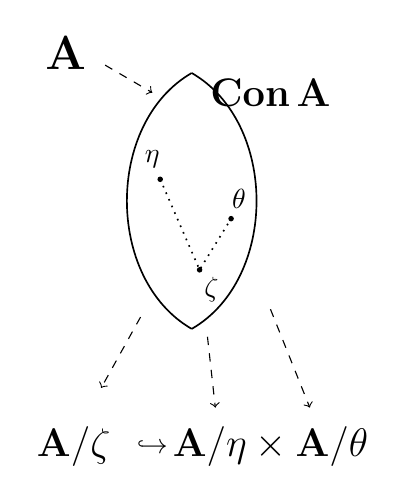
\begin{tikzpicture}[scale=.5]
          \uncover<2->{         
            \draw[font=\LARGE] (-3.2,7) node {$\bA$};
            \draw[->,dashed] (-2.2,6.7) -- (-1,6);
            \draw[->,dashed] (-1.3,.3) -- (-2.3,-1.5);
            \draw[->,dashed] (.4,-.2) -- (.6,-2);
            \draw[->,dashed] (2,.5) -- (3,-2);
          }
          
          \draw[font=\Large] (2,6) node {$\bCon \bA$};

          \draw[semithick] (0,6.5) to [out=210,in=150] (0,0);
          \draw[semithick] (0,0) to [out=30,in=-30] (0,6.5);
          %% \draw[CarnationPink] (-1,4.3) node {$\eta$};
          %% \draw[TealBlue] (1.2,3.3) node {$\theta$};
          \draw (-1,4.3) node {$\eta$};
          \draw (1.2,3.3) node {$\theta$};
          \draw (.5,1) node {$\zeta$};
          \draw[semithick, dotted] (-.8,3.8) to (.2,1.5) to (1,2.8);
          \fill (-.8,3.8) circle (2pt); 
          \fill (.2,1.5) circle (2pt); 
          \fill (1,2.8) circle (2pt); 

          \uncover<2->{         
            \draw[font=\Large] (-3,-3) node {$\bA/\zeta$}; 
            \draw (-1,-3) node {$\hookrightarrow$};
%            \draw[font=\Large] (.5,-3) node {$\bA/$};
%            \draw[font=\Large,CarnationPink] (1.5,-3) node {$\theta_0$};
%            \draw[font=\Large,orange] (1.5,-3) node {$\theta_0$};
            \draw[font=\Large] (2,-3) node {$\bA/\eta \times \bA/\theta$};
            %% \draw (2.4,-3) node {$\times$};
            %% \draw[font=\Large] (3.5,-3) node {$$};
%            \draw[font=\Large,TealBlue] (4.5,-3) node {$\theta_1$};
%            \draw[font=\Large,olivegreen] (4.5,-3) node {$\theta_1$};
          }
        \end{tikzpicture}
      \end{center}
    \end{column}
    \begin{column}{0.6\textwidth}

      The shape/structure of $\bCon \bA$
      tells us whether and how the algebra
      can be decomposed.
    \end{column}
  \end{columns}
\end{frame}

\frame[label=problem]{
  \frametitle{The Finite Lattice Representation Problem}
  %    \framesubtitle{What are the possible shapes of congruence lattices?}
  \begin{columns}
    \begin{column}{0.8\textwidth}
      There is essentially no restriction on the shape
      of a congruence lattice of an arbitrary algebra.
      \vskip3mm

      \begin{theorem}[{\small Gr\"{a}tzer-Schmidt, 1963}]
        Every algebraic lattice is isomorphic to
        the congruence lattice of an algebra.
      \end{theorem}
      \vskip3mm
      \uncover<2->{
      What if the algebra is finite?
      \begin{block}{}{{\bf Problem:}}
        Given a finite lattice $\bL$, does there exist a
        \emph{finite} algebra \bA\ such that $\bCon \bA \cong \bL$?
      \end{block}}
      \vskip2mm
      \uncover<3->{
        \begin{definition}
          We call a finite lattice \alert{representable} if it is isomorphic to
          the congruence lattice of a finite algebra.
        \end{definition}
      }
    \end{column}
  \end{columns}

}

\frame[label=classes]{
  \begin{block}{Some important classes of finite lattices}
    \begin{itemize}
    \item<1-> $\sL_0 =$ all finite lattices
    \item<1-> $\sL_1 =$ lattices isomorphic to sublattices of finite partition lattices
    \item<1-> {\color{lightgray}   $\sL_2 =$ \phantom{lattices} ...strong congruence lattices of
      finite partial algebras}
    \item<1-> $\sL_3 =$ \phantom{lattices} ...congruence lattices of finite algebras
    \item<1-> $\sL_4 = $ \phantom{lattices} ...intervals in subgroup lattices of finite groups
    \item<1-> $\sL_5 = $ \phantom{lattices} ...subgroup lattices of finite groups
    \end{itemize}
  \end{block}
  \begin{itemize}
  \item<2->Clearly 
    $\sL_0 \supseteq \sL_1 \supseteq \sL_2 \supseteq \sL_3 \supseteq \sL_4  \supseteq \sL_5$.
\note{
  \begin{itemize}
  \item $\sL_1 \supseteq \sL_3$ since $\Con \bA \leq \Eq(A)$
  \item $\sL_3 \supseteq \sL_4$ since $[H, G] \cong \Con\<G/H, G\>$.
  \item $\sL_4 \supseteq \sL_5$ obvious.
  \end{itemize}}
  \item<3->Does equality hold in each case?
    \note{$\sL_4 \neq \sL_5$ (example)}
  \item<4-> $\sL_0 = \sL_1$
    \begin{itemize}
   \item (Birkhoff, 1935) Is every lattice $\cong$
    a sublattice of a partition lattice?\\[4pt]
  \item (Whitman, 1946) Yes, {\footnotesize but proof requires infinite partition lattices.}\\[4pt]
  \item (\Pudlak\ and \Tuma, 1980) $\sL_0 = \sL_1$.\\[4pt]
    \end{itemize}
  \item<5-> {\bf Main problem:} Is $\sL_0 = \sL_3$ true? 
  \item<6-> (\Palfy\ and \Pudlak, 1980) $\sL_0 = \sL_3$ if and only if $\sL_0 = \sL_4$.\\[4pt]
\uncover<7->{This does {\bf not} say $\sL_3 = \sL_4$.  It's possible that $\sL_0 \supsetneqq \sL_3 \supsetneqq \sL_4$.}
  \end{itemize}
}


\frame[label=milestones]{
  \frametitle{Recap}
  \begin{columns}
    \begin{column}{0.8\textwidth}
      \begin{theorem}[{\small Pudl\'ak and T\r{u}ma, 1980}]
        Every finite lattice can be embedded in $\Eq(X)$ with $X$ finite.
      \end{theorem}
      In other words, $\sL_0 = \sL_1$.
      \vskip3mm
      \begin{theorem}[{\small P\'alfy and Pudl\'ak, 1980}]
        The following statements are equivalent:
        \begin{itemize}
        \item[(i)] Every finite lattice is isomorphic to
          the congruence lattice of a finite algebra.
        \item[(ii)] Every finite lattice is isomorphic to
          an interval in the subgroup lattice of a finite group.
        \end{itemize}
      \end{theorem}
      In other words, $\sL_0 = \sL_3$ if and only if $\sL_0 = \sL_4$.
    \end{column}
  \end{columns}
}


\frame[label=methods]{
  \frametitle{How to find a representation of a finite lattice}
  %% \begin{columns}
  %%   \begin{column}{0.8\textwidth}
  \begin{block}{Method 1 (use closure properties)}{}
%closure properties of the class $\sL_3$ of representable      lattices.}
%    \vskip2mm
 The class $\sL_3$ is closed under the following operations:
  \begin{itemize} %[label=$\circ$]
  \item lattice duals (Kurzweil and Netter, 1986)
  \item interval sublattices (follows from Kurzweil-Netter)
  \item  direct products (\Tuma, 1986)
  \item  ordinal sums (McKenzie, 1984; Snow, 2000)
  \item  parallel sums (Snow, 2000)
  \item certain sublattices of lattices in $\sL_3$ (Snow, 2000) \\
    {\small (namely, those
    obtained as a union of a filter and ideal)} 
  \end{itemize}
  \end{block}
  %\visible<2->{Subdirect products?}\\[4pt]
  %\visible<3->{Homomorphic images?}

}

\frame[label=methods,shrink=5]{
  \frametitle{How to find a  representation of a finite lattice}
  %% \begin{columns}
  %%   \begin{column}{0.8\textwidth}
  \begin{block}{Method 2 (use a Galois correspondence)}{} %{Find a ``closed'' concrete representation of $L$ in $\Eq(X)$.}
    \begin{itemize} %[label=$\diamond$]
    \item Fix $\theta \subseteq X\times X$, \hskip2mm $f: X^n\rightarrow X$.\\[4pt]
      Say that $f$ \alert{respects} $\theta$ and write $f(\theta) \subseteq \theta$ provided 
      \[(x_i, y_i)\in \theta \; \Rightarrow \;
      (f(x_1, \dots, x_n), f(y_1, \dots, y_n))\in \theta.\]
    \item<2-> For $L\subseteq \Eq(X)$ define
      \[
      \lambda(L) = \{f\in X^X \mid (\forall \theta \in L) \; f(\theta) \subseteq \theta \},
      \]
      the set of unary maps on $X$ which respect all relations in $L$.
      \vskip2mm
      %% \item[] For $L\leq \Eq(X)$ define
      %%   \[
      %%   \lambda(L) = \{f\in X^X: (\forall \theta \in L) \; f(\theta) \subseteq \theta \}
      %%   \]
    \item<3-> For $F\subseteq X^X$ define
      \[
      \rho(F) = \{\theta \in \Eq(X) \mid   (\forall f\in F) \; f(\theta) \subseteq \theta\},
      \]
      the set of equivalence relations on $X$ respected by all $f\in F$.
      \vskip2mm
    \item<4-> Then $L \subseteq \rho \lambda (L)$ and $\rho \lambda$ is a \emph{closure operator} on $\Sub[\Eq(X)]$.\\
      {\small (idempotent, extensive, order preserving)}
      \vskip2mm
    \item<5-> If a lattice $L\leq \Eq(X)$ is \emph{closed}, i.e. $\rho\lambda(L) = L$, then
      \[L = \Con \<X, \lambda(L)\>\]
    \end{itemize}
  \end{block}

}


%% \frame[label=methods]{
%%   \frametitle{How to find a representation of a finite lattice}
%%   \begin{block}{Method 3 (subgroup lattice interval)}{Find $L$ as an interval in a subgroup lattice of a finite group.}

%%     \vskip3mm

%%     If $H\leq G$ are finite groups, then the interval above $H$ in $Sub(G)$,
%%     \[
%%       [H,G] := \{K \mid H\leq K \leq G\},
%%       \]
%%       is isomorphic to $\Con\<G/H, G\>$.

%%   \end{block}

%%   \vskip6mm
%% \uncover<2->{
%%   \begin{block}{Method 4 (filter+ideal)}{Find $L$ as the union of a filter and ideal in a representable lattice.}

%%   \end{block}
%% }
%% }

\frame[label=methods]{
  \frametitle{How to find a representation of a finite lattice}
  \begin{block}{Method 3 (subgroup lattice interval)}{Find $L$ as an interval in a subgroup lattice of a finite group.}

    \vskip3mm

    If $H\leq G$ are finite groups, then the interval above $H$ in $Sub(G)$,
    \[
      [H,G] := \{K \mid H\leq K \leq G\},
      \]
      is isomorphic to $\Con\<G/H, G\>$.

  \end{block}

}



\frame[label=filteridealShort]{
  \frametitle{How to find a representation of a finite lattice}
  \begin{block}{Method 4 (filter+ideal)}{Find $L$ as the union of a filter and ideal in a representable lattice.}
  \end{block}

  \vskip5pt
  \begin{columns}
      \begin{column}{0.65\textwidth}
%  \begin{lemma}
    Suppose $L_0 \cong \Con \<A, F\>$, \hskip4pt 
    $\alpha, \beta \in L_0\setminus \{0, 1\}$.\\[6pt]
    \uncover<2->{Consider             
      {\color{blue} $\;L = \alpha^\uparrow \cup \beta^\downarrow$.\\[6pt] }
    }
    \uncover<3->{Then there exists a set $F' \subset A^A$ such that 
      \[
        {\color{blue} L} \cong \Con \<A, F\cup F'\>.
        \]
    }
%  \end{lemma}
      \end{column}

    \begin{column}{0.25\textwidth}
      \begin{center}
        \begin{tikzpicture}[scale=.4]
          % lat5
          \node (c) at (.5,.75)   {};
          \node (d) at (-1.5,4.5)   {};
          \node (e) at (1,2)   {};
          \node (f) at (-.75,6)   {};
                {\color<2->{blue} \node (bottom) at (0,0)  [fill, circle, inner sep=.8pt] {};
                  \node (top) at (0,8)  [fill, circle, inner sep=.8pt] {};
                  \node (alpha) at (-1.8,3)  [fill, circle, inner sep=.8pt] {};
                  \node (beta) at (1.5,4)  [fill, circle, inner sep=.8pt] {};}
                %% \uncover<4->{  
                %%   \node (theta) at (-.5,3)  [fill, circle, inner sep=.8pt] {};
                %%   \draw (-.3,3.5) node {$\theta$};
                %% }
                \draw[semithick] 
                (bottom) to [out=15, in=-15] (top) 
                (top) to [out=195, in=165] (bottom);
                     {\color<2->{blue}
                       \only<2,3>{ \draw[dotted] (c) to (d) (e) to (f);}
                       \uncover<2->{
                         \draw[dotted] (bottom) to (alpha)  (beta) to (top);
                         \draw[semithick] 
                         (alpha) to [out=30, in=-80] (top)
                         (top) to [out=205, in=105] (alpha)
                         (bottom) to [out=30, in=-80] (beta)
                         (beta) to [out=205, in=110] (bottom);
                         }
                     }
                     \draw (-2,9) node {$\uncover<2->{{\color{blue} L} \leq}  L_0$};
                           {\color<2->{blue}
                             \draw (-1.8,2.5) node {$\alpha$};
                             \draw (1.5,4.5) node {$\beta$};
                           }
        \end{tikzpicture}
      \end{center}
    \end{column}
  \end{columns}
}





\frame[label=filteridealLong,shrink=5]{
  \frametitle{Method 4}

  \begin{lemma}
    Suppose $L_0 \cong \Con \<A, F\>$, \hskip4pt 
    and $\alpha, \beta \in L_0\setminus \{0, 1\}$. \hskip6pt
    \uncover<2->{Consider             
      {\color{blue} $\;L = \alpha^\uparrow \cup \beta^\downarrow$.\\[4pt] }
    }
    \uncover<3->{There exists a set $F' \subset A^A$ such that 
      ${\color{blue} L} \cong \Con \<A, F\cup F'\>$.}
  \end{lemma}
  \vskip5pt
  \begin{columns}
    \uncover<4->{
      \begin{column}{0.65\textwidth}
        \underline{{\it Proof:}}\\
        \begin{itemize}
        \item[] 
          Fix $\theta \in L_0 \setminus {\color{blue} L}$.  Then $\alpha \nleq \theta \nleq \beta $, so
          \begin{itemize}
          \item $\exists (a,b) \in \alpha \setminus \theta$,\vskip4pt
          \item $\exists (u,v) \in \theta \setminus \beta$.
          \end{itemize}
          \vskip5pt
          Define $f_\theta :A \rightarrow A$ by
          \[
          f_\theta(x) = 
          \begin{cases}
            a & x \in u/\beta,\\
            b & x \notin u/\beta.
          \end{cases}
          \]
          Then
          \begin{itemize} %[label=$\diamond$]
          \item $(f_\theta(u),f_\theta(v)) = (a,b) \notin \theta$, so $f_\theta(\theta) \nsubseteq \theta$,\vskip2pt
          \item $\ker f_\theta \geq \beta$, so $f_\theta(\gamma) \subseteq \gamma$ for all $\gamma \leq \beta$,\vskip2pt
          \item $f_\theta(A) \subseteq \{a,b\}$, so $f_\theta(\gamma) \subseteq \gamma$ for all $\gamma \geq \alpha$.
          \end{itemize}
          \vskip5pt
          Let $F' = \{f_\theta : \theta \in L_0\setminus {\color{blue}L}\}$.
        \end{itemize}

      \end{column}
    }
    \begin{column}{0.25\textwidth}
      \begin{center}
        \begin{tikzpicture}[scale=.4]
          % lat5
          \node (c) at (.5,.75)   {};
          \node (d) at (-1.5,4.5)   {};
          \node (e) at (1,2)   {};
          \node (f) at (-.75,6)   {};
                {\color<2->{blue} \node (bottom) at (0,0)  [fill, circle, inner sep=.8pt] {};
                  \node (top) at (0,8)  [fill, circle, inner sep=.8pt] {};
                  \node (alpha) at (-1.8,3)  [fill, circle, inner sep=.8pt] {};
                  \node (beta) at (1.5,4)  [fill, circle, inner sep=.8pt] {};}
                \uncover<4->{  
                  \node (theta) at (-.5,3)  [fill, circle, inner sep=.8pt] {};
                  \draw (-.3,3.5) node {$\theta$};
                }
                \draw[semithick] 
                (bottom) to [out=15, in=-15] (top) 
                (top) to [out=195, in=165] (bottom);
                     {\color<2->{blue}
                       \only<2,3>{ \draw[dotted] (c) to (d) (e) to (f);}
                       \uncover<2->{
                         \draw[dotted] (bottom) to (alpha)  (beta) to (top);
                         \draw[semithick] 
                         (alpha) to [out=30, in=-80] (top)
                         (top) to [out=205, in=105] (alpha)
                         (bottom) to [out=30, in=-80] (beta)
                         (beta) to [out=205, in=110] (bottom);
                         }
                     }
                     \draw (-2,9) node {$\uncover<2->{{\color{blue} L} \leq}  L_0$};
                           {\color<2->{blue}
                             \draw (-1.8,2.5) node {$\alpha$};
                             \draw (1.5,4.5) node {$\beta$};
                           }
        \end{tikzpicture}
      \end{center}
    \end{column}
  \end{columns}
}





\frame[label=knownresults]{
  \frametitle{Lattices with at most 6 elements are representable.}
  
  \begin{center}
    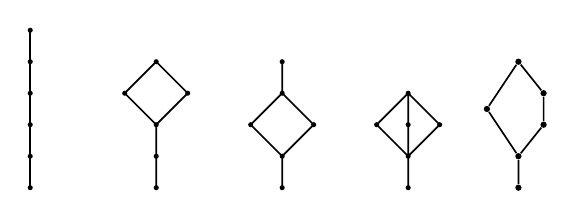
\begin{tikzpicture}[scale=.4]

      % lat1
      \foreach \j in {1,...,6}{ 
        \path (0,\j) coordinate (0\j); \fill (0\j) circle (2.3pt); 
      }
      \draw[semithick] (01) to (06);

      % lat2
      \foreach \j in {1,2,3,5}{ 
        \path (4,\j) coordinate (4\j); \fill (4\j) circle (2.3pt); 
      }
      \path (3,4) coordinate (34); \fill (34) circle (2.3pt);
      \path (5,4) coordinate (54); \fill (54) circle (2.3pt);
      \draw[semithick] (41) to (43) to (34) to (45) to (54) to (43);

      % lat3
      \foreach \j in {1,2,4,5} { 
        \path (8,\j) coordinate (8\j); \fill (8\j) circle (2.3pt); 
      }
      \path (7,3) coordinate (73); \fill (73) circle (2.3pt);
      \path (9,3) coordinate (93); \fill (93) circle (2.3pt);
      \draw[semithick] (81) to (82) to (73) to (84) to (85) (84) to (93) to (82);

      % lat4
      \foreach \j in {1,...,4} { 
        \path (12,\j) coordinate (12\j); \fill (12\j) circle (2.3pt); 
      }
      \path (11,3) coordinate (113); \fill (113) circle (2.3pt);
      \path (13,3) coordinate (133); \fill (133) circle (2.3pt);
      \draw[semithick] (121) to (124) to (113) to (122) to (133) to (124);

      % lat5
      \foreach \j in {1,2,5} {
        \node (15\j) at (15.5,\j) [fill,circle,inner sep=.8pt] {};
      }
      \foreach \j in {3,4} {
        \node (15\j) at (16.3,\j) [fill,circle,inner sep=.8pt] {};
      }
      \node (1435) at (14.5,3.5) [fill,circle,inner sep=.8pt] {};
      \draw[semithick] (151) to (152) to (153) to (154) to (155) to (1435) to (152);

    \end{tikzpicture}
  \end{center}

  \begin{center}
    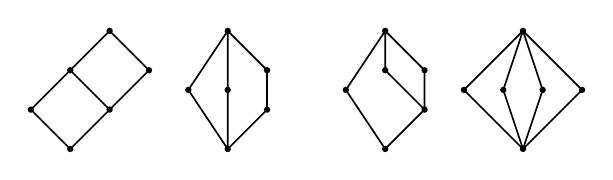
\begin{tikzpicture}[scale=.5]

      % lat6
      \path (0,1) coordinate (01); \fill (01) circle (2.3pt);
      \foreach \j in {0,2} {
        \path (1,\j) coordinate (1\j); \fill (1\j) circle (2.3pt); 
      }
      \foreach \j in {1,3} {
        \path (2,\j) coordinate (2\j); \fill (2\j) circle (2.3pt); 
      }
      \path (3,2) coordinate (32); \fill (32) circle (2.3pt);
      \draw[semithick] (10) to (01) to (23) to (32) to (10) (21) to (12);

      % lat7
      \foreach \j in {0,3} {
        \path (5,\j) coordinate (5\j); \fill (5\j) circle (2.3pt); 
      }
      \path (5,1.5) coordinate (51); \fill (51) circle (2.3pt);
      \path (4,1.5) coordinate (41); \fill (41) circle (2.3pt);
      \foreach \j in {1,2} {
        \path (6,\j) coordinate (6\j); \fill (6\j) circle (2.3pt); 
      }
      \draw[semithick] (50) to (41) to (53) to (50) to (61) to (62) to (53);
      
      % lat8
      % \foreach \i in {7,8,9} 
      \foreach \i in {9,10} {
        \path (\i,2) coordinate (\i2); \fill (\i2) circle (2.3pt); 
      }
      \path (8,1.5) coordinate (82); \fill (82) circle (2.3pt);
      \path (9,0) coordinate (90); \fill (90) circle (2.3pt);
      \path (9,3) coordinate (93); \fill (93) circle (2.3pt);
      \path (10,1) coordinate (101); \fill (101) circle (2.3pt);
      \draw[semithick] (90) to (82) to (93) to (92) to (101) to (90) (101) to (102) to (93);

      % lat9
      \foreach \j in {0,3}{
        \path (12.5,\j) coordinate (125\j); 
        \fill (125\j) circle (2.3pt);
      }
      \foreach \i in {11,...,14}{
        \path (\i,1.5) coordinate (\i15); 
        \fill (\i15) circle (2.3pt);
        \draw[semithick] (\i15) to (1250);
        \draw[semithick] (\i15) to (1253);
      }

    \end{tikzpicture}
  \end{center}
  \setbeamercovered{transparent}
  \begin{center}
    {\scalefont{.8}
      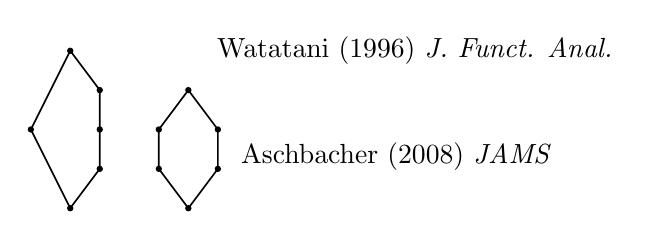
\begin{tikzpicture}[scale=.5]
%        \uncover<2->{      % lat10
          \foreach \j in {1,5}{
            \path (3.25,\j) coordinate (4\j); \fill (4\j) circle (2.3pt); 
          }
          \foreach \j in {2,...,4}{
            \path (4,\j) coordinate (4\j); \fill (4\j) circle (2.3pt); 
          }
          \path (2.25,3) coordinate (33); \fill (33) circle (2.3pt);
          \draw[semithick] (41) to (42) to (44) to (45) to (33) to (41);

          % lat11
          \foreach \j in {2,3}{
            \path (5.5,\j) coordinate (5\j); \fill (5\j) circle (2.3pt);
            \path (7,\j) coordinate (7\j); \fill (7\j) circle (2.3pt); 
          }
          \foreach \j in {1,4} {
            \path (6.25,\j) coordinate (6\j); \fill (6\j) circle (2.3pt);
          }
          \draw[semithick] (61) to (52) to (53) to (64) to (73) to (72) to (61);
%    }
        \uncover<1->{
          \draw (12,5) node {Watatani (1996) {\it J. Funct. Anal.}};
        }
        \uncover<1->{
          \draw (11.5,2.3) node {Aschbacher (2008) {\it JAMS}};
        }

      \end{tikzpicture}
    }
  \end{center}
  \note{There are 15 six element lattices.  These are all of them modulo duals.}
  \uncover<1->{
    {\bf Theorem:} {\it Every lattice with at most 6 elements is
      an interval in the \\ 
      \hskip15.5mm subgroup lattice of a finite group.}}
}


%%%%%%%%%%  Start of 7 element lattice section  %%%%%%%%%%%%%%%%%%

\frame[label=results]{
  \frametitle{Are all lattices with at most 7 elements representable?}
  %{\color{gray}As of February 2011...}
             {\it As of February 2011...}

             \vspace{-.5cm}

             \begin{center}
               \includegraphics[height=2.3in]{Sevens}
             \end{center}
             \hfill {\small {\it Figure courtesy of Peter Jipsen.}}
}  


\begin{frame}[label=knownresults,shrink=5]{
    Are all lattices with at most 7 elements representable?}
  \note{There are 53 seven element lattices.  We found representations for 43 of
    them without too much trouble.  The last 10 were hard.}
  \begin{columns}
    \begin{column}{0.2\textwidth}
      \begin{center}
        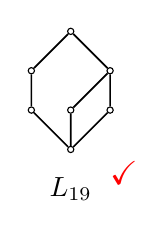
\begin{tikzpicture}[scale=.5]

          % L19
        \node (bottom) at (0,0)  [draw, circle, inner sep=\dotsize] {};
        \node (top) at (0,3)  [draw, circle, inner sep=\dotsize] {};
        \node (11) at (1,1)  [draw, circle, inner sep=\dotsize] {};
        \node (n11) at (-1,1)  [draw, circle, inner sep=\dotsize] {};
        \node (12) at (1,2)  [draw, circle, inner sep=\dotsize] {};
        \node (n12) at (-1,2)  [draw, circle, inner sep=\dotsize] {};
        \node (01) at (0,1)  [draw, circle, inner sep=\dotsize] {};

        \draw[semithick] (bottom) to (11) to (12) to (top) to (n12) to (n11) to (bottom) to (01) to (12);

          \draw (0,-1) node {$L_{19}$};
          \visible<2->{ {\color{red}\draw[font=\large] (1,-.6) node{$\text{\rlap{$\checkmark$}}$ };}
            %\draw[font=\large] (2.5,-.6) node { {\footnotesize Jipsen}};
          }

        \end{tikzpicture}
      \end{center}
    \end{column}
    \begin{column}{0.2\textwidth}
      \begin{center}
        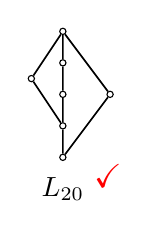
\begin{tikzpicture}[scale=.4]
          % L20
      \foreach \j in {0,...,4}
      {
        \node (0\j) at (0,\j)  [draw, circle, inner sep=\dotsize] {};
      }
      \node (152) at (1.5,2)  [draw, circle, inner sep=\dotsize] {};
      \node (n125) at (-1,2.5)  [draw, circle, inner sep=\dotsize] {};
      \draw[semithick] (01) to (02) to (03) to (04) to (n125) to (01) to (00) to (152) to (04);

          \draw (0,-1) node {$L_{20}$};
          \visible<2->{        {\color{red}\draw[font=\large] (1,-.6) node{$\text{\rlap{$\checkmark$}}$ };}
            %\draw[font=\large] (3,-.6) node { {\footnotesize Jipsen}};
          }
        \end{tikzpicture}
      \end{center}
    \end{column}
  \end{columns}

  \begin{columns}
    \begin{column}{0.2\textwidth}
      \begin{center}
        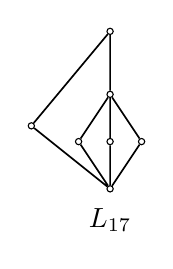
\begin{tikzpicture}[scale=.4]

          
        \node (bottom) at (0,0)  [draw, circle, inner sep=\dotsize] {};
        \node (top) at (0,5)  [draw, circle, inner sep=\dotsize] {};
        \node (n115) at (-1,1.5)  [draw, circle, inner sep=\dotsize] {};
        \node (015) at (0,1.5)  [draw, circle, inner sep=\dotsize] {};
        \node (115) at (1,1.5)  [draw, circle, inner sep=\dotsize] {};
        \node (n252) at (-2.5,2)  [draw, circle, inner sep=\dotsize] {};
        \node (03) at (0,3)  [draw, circle, inner sep=\dotsize] {};
        \draw[semithick] 
        (bottom) to (n252) to (top)
        (bottom) to (n115) to (03) to (115) to
        (bottom) to (015) to (03) to (top);
       %\draw (-4.5,2.2) node {$L \cong$};



          \draw (0,-1) node {$L_{17}$};
        \end{tikzpicture}
      \end{center}
    \end{column}

    \begin{column}{0.2\textwidth}
      \begin{center}
        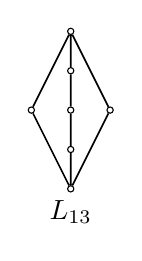
\begin{tikzpicture}[scale=.5]

          %\newcommand{\dotsize}{1};
\node (0) at (0,0) [draw, circle,inner sep=\dotsize] {};
\node (1) at (-0,1) [draw, circle, inner sep=\dotsize] {};
\node (2) at (1,2) [draw, circle, inner sep=\dotsize] {};
\node (3) at (-1,2) [draw, circle, inner sep=\dotsize] {};
\node (4) at (-0,2) [draw, circle, inner sep=\dotsize] {};
\node (5) at (-0,3) [draw, circle, inner sep=\dotsize] {};
\node (6) at (-0,4) [draw, circle, inner sep=\dotsize] {};
%\draw[font=\scriptsize] (0,-.5) node {[A4, (C2 x C2 x C2 x C2) : A5]};
%\draw[font=\scriptsize] (0,-1) node {SmallGroup(960,11358) Index 80};

\draw[semithick]
(0) to (1)
(0) to (2)
(0) to (3)
(1) to (4)
(2) to (6)
(3) to (6)
(4) to (5)
(5) to (6);

          \draw (0,-.6) node {$L_{13}$};

        \end{tikzpicture}
      \end{center}
    \end{column}

    \begin{column}{0.2\textwidth}
      \begin{center}
        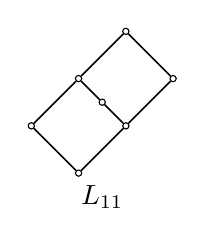
\begin{tikzpicture}[scale=.3]

          % L11 aka L3 
        \node (bottom) at (0,0)  [draw, circle, inner sep=\dotsize] {};
        \node (top) at (2,6)  [draw, circle, inner sep=\dotsize] {};
        \node (n22) at (-2,2)  [draw, circle, inner sep=\dotsize] {};
        \node (22) at (2,2)  [draw, circle, inner sep=\dotsize] {};
        \node (13) at (1,3)  [draw, circle, inner sep=\dotsize] {};
        \node (04) at (0,4)  [draw, circle, inner sep=\dotsize] {};
        \node (44) at (4,4)  [draw, circle, inner sep=\dotsize] {};

        \draw[semithick] (bottom) to (22) to (44) to (top) to (04) to (13) to (22)
        (bottom) to (n22) to (04);
  
          \draw (1,-1) node {$L_{11}$};
          %{$L_{11}$ {\small (aka $L_3$)}};

        \end{tikzpicture}
      \end{center}
    \end{column}

  \end{columns}


  \begin{columns}

    \begin{column}{0.2\textwidth}
      \begin{center}
        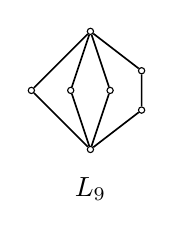
\begin{tikzpicture}[scale=.5]

          %% ``L9'' is the pentegon with two extra wings.
      \foreach \j in {0,3} 
      { \node (7\j) at (6.5,\j)  [draw, circle, inner sep=\dotsize] {};}
      \node (71) at (7,1.5)  [draw, circle, inner sep=\dotsize] {};
      \node (61) at (6,1.5)  [draw, circle, inner sep=\dotsize] {};
      \node (51) at (5,1.5)  [draw, circle, inner sep=\dotsize] {};
      \foreach \j in {1,2} 
      { \node (8\j) at (7.8,\j)  [draw, circle, inner sep=\dotsize] {};}
      \draw[semithick] (70) to (51) to (73) to (61) to (70) to (71) to (73) to
      (82) to (81) to (70);
      

          \draw (6.5,-1) node {$L_{9}$};

        \end{tikzpicture}
      \end{center}
    \end{column}


    \begin{column}{0.2\textwidth}
      \begin{center}
        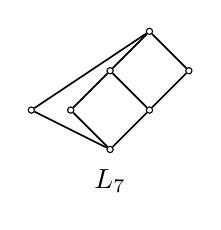
\begin{tikzpicture}[scale=.5]

          %%  The elusive winged-2x3 %%
      \node (01) at (0,1)  [draw, circle, inner sep=\dotsize] {};
      \foreach \j in {0,2} 
      { \node (1\j) at (1,\j)  [draw, circle, inner sep=\dotsize] {};}

      \foreach \j in {1,3} 
      { \node (2\j) at (2,\j)  [draw, circle, inner sep=\dotsize] {};}
      { \node (32) at (3,2)  [draw, circle, inner sep=\dotsize] {};}
      \draw[semithick] (10) to (01) to (12) to (23) to (32) to (21) to (10) (21) to (12);
      { \node (m11) at (-1,1)  [draw, circle, inner sep=\dotsize] {};}
      \draw[semithick] (10) to (m11) to (23);


          \draw (1,-.8) node {$L_7$};

        \end{tikzpicture}
      \end{center}
    \end{column}
  \end{columns}
\end{frame}


\begin{frame}[label=knownresults,shrink=5]{Finding representations...}
  \framesubtitle{...as intervals in subgroup lattices}

  \begin{columns}
    \begin{column}{0.2\textwidth}
      \begin{center}
        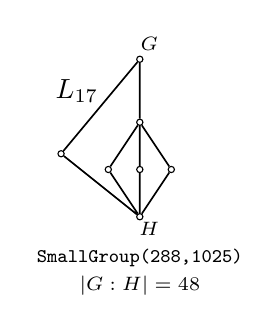
\begin{tikzpicture}[scale=.4]

          
        \node (bottom) at (0,0)  [draw, circle, inner sep=\dotsize] {};
        \node (top) at (0,5)  [draw, circle, inner sep=\dotsize] {};
        \node (n115) at (-1,1.5)  [draw, circle, inner sep=\dotsize] {};
        \node (015) at (0,1.5)  [draw, circle, inner sep=\dotsize] {};
        \node (115) at (1,1.5)  [draw, circle, inner sep=\dotsize] {};
        \node (n252) at (-2.5,2)  [draw, circle, inner sep=\dotsize] {};
        \node (03) at (0,3)  [draw, circle, inner sep=\dotsize] {};
        \draw[semithick] 
        (bottom) to (n252) to (top)
        (bottom) to (n115) to (03) to (115) to
        (bottom) to (015) to (03) to (top);
       %\draw (-4.5,2.2) node {$L \cong$};




          \draw (-2,4) node {$L_{17}$};
          \uncover<2->{
            \draw[font=\scriptsize] (0.3,5.5) node {$G$};
            \draw[font=\scriptsize] (0.3,-.4) node { $H$};
            \draw[font=\scriptsize] (0,-1.3) node {{\tt SmallGroup(288,1025)}};
            \draw[font=\scriptsize] (0,-2.2) node { $|G:H|=48$};
          }

        \end{tikzpicture}
      \end{center}
    \end{column}

    \uncover<2->{
      \begin{column}{0.6\textwidth}
        \begin{itemize}
        \item 
          The group $G = (A_4 \times A_4) \rtimes C_2$ has a subgroup $H\cong S_3$ such
          that $[H,G]\cong L_{17}$.
          \vskip10pt
        \item<2-> ...so the dual $L_{16}$ is also representable.
          %% \\[8pt]
          %%   {\small $L_{16}$ can be embedded above diagonal of the direct power of
          %%     a simple group,
          %%     \[L_{16} \hookrightarrow [D,S^{48}] \cong \Eq(48)^{dual}.\]  
          %%     Add the group operations $G$ which closed $L_{17}$.
          %%     %, and $L_{16}$ appears as an upper interval in $S^{48} \rtimes G$.
          %%   }

        \end{itemize}
      \end{column}
    }
  \end{columns}

  \begin{columns}
    \begin{column}{0.3\textwidth}
      \begin{center}
        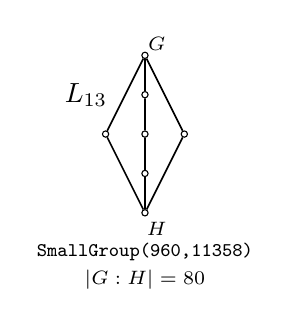
\begin{tikzpicture}[scale=.5]

          %\newcommand{\dotsize}{1};
\node (0) at (0,0) [draw, circle,inner sep=\dotsize] {};
\node (1) at (-0,1) [draw, circle, inner sep=\dotsize] {};
\node (2) at (1,2) [draw, circle, inner sep=\dotsize] {};
\node (3) at (-1,2) [draw, circle, inner sep=\dotsize] {};
\node (4) at (-0,2) [draw, circle, inner sep=\dotsize] {};
\node (5) at (-0,3) [draw, circle, inner sep=\dotsize] {};
\node (6) at (-0,4) [draw, circle, inner sep=\dotsize] {};
%\draw[font=\scriptsize] (0,-.5) node {[A4, (C2 x C2 x C2 x C2) : A5]};
%\draw[font=\scriptsize] (0,-1) node {SmallGroup(960,11358) Index 80};

\draw[semithick]
(0) to (1)
(0) to (2)
(0) to (3)
(1) to (4)
(2) to (6)
(3) to (6)
(4) to (5)
(5) to (6);


          \draw (-1.5,3) node {$L_{13}$};
          \uncover<3->{
            \draw[font=\scriptsize] (0.3,4.3) node {$G$};
            \draw[font=\scriptsize] (0.3,-.4) node { $H$};
            \draw[font=\scriptsize] (0,-1) node {{\tt SmallGroup(960,11358)}};
            \draw[font=\scriptsize] (0,-1.7) node {$|G:H|=80$};
          }
        \end{tikzpicture}
      \end{center}
    \end{column}
    \begin{column}{0.65\textwidth}
      \begin{itemize}
      \item<3-> 
        The group $G = (C_2 \times C_2 \times C_2 \times C_2) \rtimes A_5$
        has a subgroup $H\cong A_4$ such that $[H,G]\cong L_{13}$.
      \end{itemize}
    \end{column}
  \end{columns}


\end{frame}


%\begin{frame}[label=knownresults,shrink=5]{Finding representations...}
\begin{frame}[label=knownresultsdrop,shrink=5]{
    Are all lattices with at most 7 elements representable?}

  \begin{columns}
    \begin{column}{0.2\textwidth}
      \begin{center}
        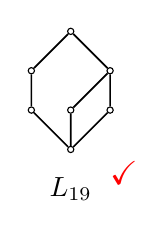
\begin{tikzpicture}[scale=.5]

          % L19
        \node (bottom) at (0,0)  [draw, circle, inner sep=\dotsize] {};
        \node (top) at (0,3)  [draw, circle, inner sep=\dotsize] {};
        \node (11) at (1,1)  [draw, circle, inner sep=\dotsize] {};
        \node (n11) at (-1,1)  [draw, circle, inner sep=\dotsize] {};
        \node (12) at (1,2)  [draw, circle, inner sep=\dotsize] {};
        \node (n12) at (-1,2)  [draw, circle, inner sep=\dotsize] {};
        \node (01) at (0,1)  [draw, circle, inner sep=\dotsize] {};

        \draw[semithick] (bottom) to (11) to (12) to (top) to (n12) to (n11) to (bottom) to (01) to (12);

          \draw (0,-1) node {$L_{19}$};
                {\color{red}\draw[font=\large] (1,-.6) node{$\text{\rlap{$\checkmark$}}$ };}
                %\draw[font=\large] (2.5,-.6) node { {\footnotesize Jipsen}};

        \end{tikzpicture}
      \end{center}
    \end{column}
    \begin{column}{0.2\textwidth}
      \begin{center}
        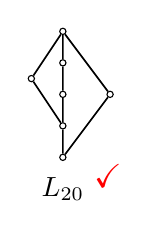
\begin{tikzpicture}[scale=.4]
          % L20
      \foreach \j in {0,...,4}
      {
        \node (0\j) at (0,\j)  [draw, circle, inner sep=\dotsize] {};
      }
      \node (152) at (1.5,2)  [draw, circle, inner sep=\dotsize] {};
      \node (n125) at (-1,2.5)  [draw, circle, inner sep=\dotsize] {};
      \draw[semithick] (01) to (02) to (03) to (04) to (n125) to (01) to (00) to (152) to (04);

          \draw (0,-1) node {$L_{20}$};
                {\color{red}\draw[font=\large] (1,-.6) node{$\text{\rlap{$\checkmark$}}$ };}
                %\draw[font=\large] (3,-.6) node { {\footnotesize Jipsen}};
        \end{tikzpicture}
      \end{center}
    \end{column}
  \end{columns}

  \begin{columns}
    \begin{column}{0.2\textwidth}
      \begin{center}
        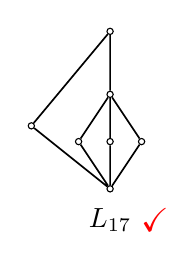
\begin{tikzpicture}[scale=.4]

          
        \node (bottom) at (0,0)  [draw, circle, inner sep=\dotsize] {};
        \node (top) at (0,5)  [draw, circle, inner sep=\dotsize] {};
        \node (n115) at (-1,1.5)  [draw, circle, inner sep=\dotsize] {};
        \node (015) at (0,1.5)  [draw, circle, inner sep=\dotsize] {};
        \node (115) at (1,1.5)  [draw, circle, inner sep=\dotsize] {};
        \node (n252) at (-2.5,2)  [draw, circle, inner sep=\dotsize] {};
        \node (03) at (0,3)  [draw, circle, inner sep=\dotsize] {};
        \draw[semithick] 
        (bottom) to (n252) to (top)
        (bottom) to (n115) to (03) to (115) to
        (bottom) to (015) to (03) to (top);
       %\draw (-4.5,2.2) node {$L \cong$};



          \draw (0,-1) node {$L_{17}$};
                {\color{red}\draw[font=\large] (1,-1) node{$\text{\rlap{$\checkmark$}}$ };}


        \end{tikzpicture}
      \end{center}
    \end{column}

    \begin{column}{0.2\textwidth}
      \begin{center}
        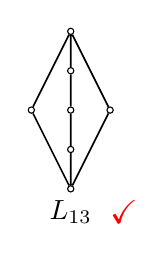
\begin{tikzpicture}[scale=.5]

          %\newcommand{\dotsize}{1};
\node (0) at (0,0) [draw, circle,inner sep=\dotsize] {};
\node (1) at (-0,1) [draw, circle, inner sep=\dotsize] {};
\node (2) at (1,2) [draw, circle, inner sep=\dotsize] {};
\node (3) at (-1,2) [draw, circle, inner sep=\dotsize] {};
\node (4) at (-0,2) [draw, circle, inner sep=\dotsize] {};
\node (5) at (-0,3) [draw, circle, inner sep=\dotsize] {};
\node (6) at (-0,4) [draw, circle, inner sep=\dotsize] {};
%\draw[font=\scriptsize] (0,-.5) node {[A4, (C2 x C2 x C2 x C2) : A5]};
%\draw[font=\scriptsize] (0,-1) node {SmallGroup(960,11358) Index 80};

\draw[semithick]
(0) to (1)
(0) to (2)
(0) to (3)
(1) to (4)
(2) to (6)
(3) to (6)
(4) to (5)
(5) to (6);

          \draw (0,-.6) node {$L_{13}$};
                {\color{red}\draw[font=\large] (1,-.6) node{$\text{\rlap{$\checkmark$}}$ };}

        \end{tikzpicture}
      \end{center}
    \end{column}

    \begin{column}{0.2\textwidth}
      \begin{center}
        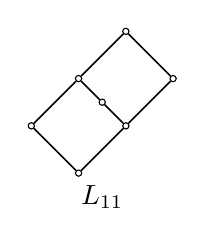
\begin{tikzpicture}[scale=.3]

          % L11 aka L3 
        \node (bottom) at (0,0)  [draw, circle, inner sep=\dotsize] {};
        \node (top) at (2,6)  [draw, circle, inner sep=\dotsize] {};
        \node (n22) at (-2,2)  [draw, circle, inner sep=\dotsize] {};
        \node (22) at (2,2)  [draw, circle, inner sep=\dotsize] {};
        \node (13) at (1,3)  [draw, circle, inner sep=\dotsize] {};
        \node (04) at (0,4)  [draw, circle, inner sep=\dotsize] {};
        \node (44) at (4,4)  [draw, circle, inner sep=\dotsize] {};

        \draw[semithick] (bottom) to (22) to (44) to (top) to (04) to (13) to (22)
        (bottom) to (n22) to (04);
  \draw (1,-1) node {$L_{11}$};

        \end{tikzpicture}
      \end{center}
    \end{column}

  \end{columns}

  \begin{columns}

    \begin{column}{0.2\textwidth}
      \begin{center}
        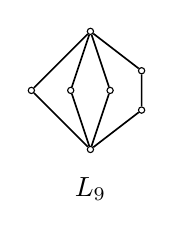
\begin{tikzpicture}[scale=.5]

          %% ``L9'' is the pentegon with two extra wings.
      \foreach \j in {0,3} 
      { \node (7\j) at (6.5,\j)  [draw, circle, inner sep=\dotsize] {};}
      \node (71) at (7,1.5)  [draw, circle, inner sep=\dotsize] {};
      \node (61) at (6,1.5)  [draw, circle, inner sep=\dotsize] {};
      \node (51) at (5,1.5)  [draw, circle, inner sep=\dotsize] {};
      \foreach \j in {1,2} 
      { \node (8\j) at (7.8,\j)  [draw, circle, inner sep=\dotsize] {};}
      \draw[semithick] (70) to (51) to (73) to (61) to (70) to (71) to (73) to
      (82) to (81) to (70);
      

          \draw (6.5,-1) node {$L_{9}$};

        \end{tikzpicture}
      \end{center}
    \end{column}


    \begin{column}{0.2\textwidth}
      \begin{center}
        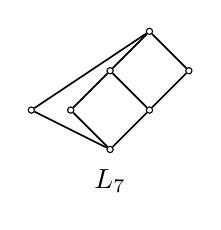
\begin{tikzpicture}[scale=.5]

          %%  The elusive winged-2x3 %%
      \node (01) at (0,1)  [draw, circle, inner sep=\dotsize] {};
      \foreach \j in {0,2} 
      { \node (1\j) at (1,\j)  [draw, circle, inner sep=\dotsize] {};}

      \foreach \j in {1,3} 
      { \node (2\j) at (2,\j)  [draw, circle, inner sep=\dotsize] {};}
      { \node (32) at (3,2)  [draw, circle, inner sep=\dotsize] {};}
      \draw[semithick] (10) to (01) to (12) to (23) to (32) to (21) to (10) (21) to (12);
      { \node (m11) at (-1,1)  [draw, circle, inner sep=\dotsize] {};}
      \draw[semithick] (10) to (m11) to (23);


          \draw (1,-.8) node {$L_7$};

        \end{tikzpicture}
      \end{center}
    \end{column}
  \end{columns}
\end{frame}



\begin{frame}[label=knownresults,shrink=5]{Finding representations...}
  \framesubtitle{...using subgroup lattice intervals and the filter+ideal lemma.}

  %\uncover<2->{
  \begin{columns}
    \begin{column}{0.2\textwidth}
      \begin{center}
        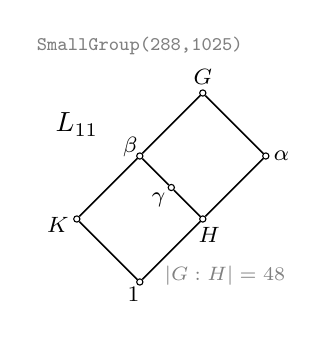
\begin{tikzpicture}[scale=.4]
          % L11 aka L3 
        \node (bottom) at (0,0)  [draw, circle, inner sep=\dotsize] {};
        \node (top) at (2,6)  [draw, circle, inner sep=\dotsize] {};
        \node (n22) at (-2,2)  [draw, circle, inner sep=\dotsize] {};
        \node (22) at (2,2)  [draw, circle, inner sep=\dotsize] {};
        \node (13) at (1,3)  [draw, circle, inner sep=\dotsize] {};
        \node (04) at (0,4)  [draw, circle, inner sep=\dotsize] {};
        \node (44) at (4,4)  [draw, circle, inner sep=\dotsize] {};

        \draw[semithick] (bottom) to (22) to (44) to (top) to (04) to (13) to (22)
        (bottom) to (n22) to (04);
;
          \draw (-2,5) node {$L_{11}$};
          \uncover<2->{
            \draw[font=\footnotesize] 
            (2,6.5) node {$G$} (2.2,1.5) node {$H$} (-.2,-.4) node {$1$}
            (4.5,4) node {$\alpha$} (-.3,4.3) node {$\beta$} (.6,2.6) node {$\gamma$};
                 {\color{gray} \draw[font=\scriptsize] (0,7.5) node {{\tt SmallGroup(288,1025)}};}
                 {\color{gray} \draw[font=\scriptsize] (2.7,.2) node {$|G:H|=48$};}
          }
          \uncover<3->{
            \draw[font=\footnotesize]  (-2.6,1.8) node {$K$};
          }
        \end{tikzpicture}
      \end{center}
    \end{column}
    \begin{column}{0.6\textwidth}
      \vskip1cm
      \begin{itemize}
      \item<2-> 
        Let $G=(A_4 \times A_4) \rtimes C_2$. %\hskip6pt ($|G| = 216$).
      \item<2-> $G$ has a subgroup $H \cong C_6$ with $[H, G] \cong N_5$. \hskip6pt %($|G:H| = 36$).
      \item<2-> Let $[H, G] = \{H, \alpha, \beta, \gamma, G\} \cong N_5$.\vskip6pt
      \item<3-> $\Sub(G)$ is a congruence lattice, so
        if there exists a subgroup $K \succ 1$, below $\beta$ and not below $\gamma$, 
        then \[L_{11} \cong K^\downarrow \cup H^\uparrow.\]
      \end{itemize}
    \end{column}
  \end{columns}
  %}

  \uncover<4->{
    \begin{columns}
      \begin{column}{0.2\textwidth}
        \begin{center}
          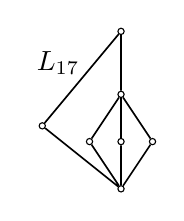
\begin{tikzpicture}[scale=.4]
            
        \node (bottom) at (0,0)  [draw, circle, inner sep=\dotsize] {};
        \node (top) at (0,5)  [draw, circle, inner sep=\dotsize] {};
        \node (n115) at (-1,1.5)  [draw, circle, inner sep=\dotsize] {};
        \node (015) at (0,1.5)  [draw, circle, inner sep=\dotsize] {};
        \node (115) at (1,1.5)  [draw, circle, inner sep=\dotsize] {};
        \node (n252) at (-2.5,2)  [draw, circle, inner sep=\dotsize] {};
        \node (03) at (0,3)  [draw, circle, inner sep=\dotsize] {};
        \draw[semithick] 
        (bottom) to (n252) to (top)
        (bottom) to (n115) to (03) to (115) to
        (bottom) to (015) to (03) to (top);
       %\draw (-4.5,2.2) node {$L \cong$};


;
            \draw (-2,4) node {$L_{17}$};
          \end{tikzpicture}
        \end{center}
      \end{column}
      \begin{column}{0.3\textwidth}
        \begin{center}
          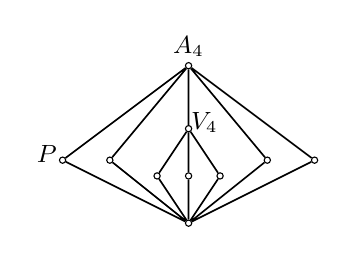
\begin{tikzpicture}[scale=.4]
                    \node (bottom) at (0,0)  [draw, circle, inner sep=\dotsize] {};
        \node (top) at (0,5)  [draw, circle, inner sep=\dotsize] {};
        \node (n115) at (-1,1.5)  [draw, circle, inner sep=\dotsize] {};
        \node (015) at (0,1.5)  [draw, circle, inner sep=\dotsize] {};
        \node (115) at (1,1.5)  [draw, circle, inner sep=\dotsize] {};
        \node (n252) at (-2.5,2)  [draw, circle, inner sep=\dotsize] {};
        \node (252) at (2.5,2)  [draw, circle, inner sep=\dotsize] {};
        \node (n42) at (-4,2)  [draw, circle, inner sep=\dotsize] {};
        \node (42) at (4,2)  [draw, circle, inner sep=\dotsize] {};
        \node (03) at (0,3)  [draw, circle, inner sep=\dotsize] {};
        \draw[semithick] 
        (bottom) to (42) to (top) to (n42) to 
        (bottom) to (n252) to (top) to (252) to 
        (bottom) to (n115) to (03) to (115) to
        (bottom) to (015) to (03) to (top);

            \draw[font=\small] (0,5.6) node {$A_4$};
            \draw[font=\small] (.5,3.2) node {$V_4$};
            \draw[font=\small] (-4.5,2.2) node {$P$};
          \end{tikzpicture}
        \end{center}
      \end{column}
      \begin{column}{0.45\textwidth}
        \begin{itemize}
        \item $\Sub(A_4)$ is a congruence lattice 
          {\footnotesize (of $A_4$ acting regularly on itself).}\vskip6pt
        \item Therefore, 
          \[L_{17} \cong V_4^\downarrow \cup P^\uparrow\]
          is a congruence lattice.
        \end{itemize}
      \end{column}
  }

    \end{columns}

\end{frame}


\begin{frame}[label=knownresults,shrink=5]{
    Are all lattices with at most 7 elements representable?}
  \begin{columns}
    \begin{column}{0.2\textwidth}
      \begin{center}
        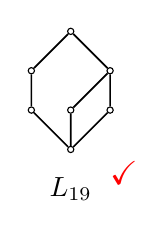
\begin{tikzpicture}[scale=.5]

          % L19
        \node (bottom) at (0,0)  [draw, circle, inner sep=\dotsize] {};
        \node (top) at (0,3)  [draw, circle, inner sep=\dotsize] {};
        \node (11) at (1,1)  [draw, circle, inner sep=\dotsize] {};
        \node (n11) at (-1,1)  [draw, circle, inner sep=\dotsize] {};
        \node (12) at (1,2)  [draw, circle, inner sep=\dotsize] {};
        \node (n12) at (-1,2)  [draw, circle, inner sep=\dotsize] {};
        \node (01) at (0,1)  [draw, circle, inner sep=\dotsize] {};

        \draw[semithick] (bottom) to (11) to (12) to (top) to (n12) to (n11) to (bottom) to (01) to (12);

          \draw (0,-1) node {$L_{19}$};
                {\color{red}\draw[font=\large] (1,-.6) node{$\text{\rlap{$\checkmark$}}$ };}
                %\draw[font=\footnotesize] (2.5,-.6) node { Jipsen};

        \end{tikzpicture}
      \end{center}
    \end{column}
    \begin{column}{0.2\textwidth}
      \begin{center}
        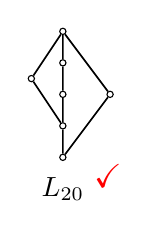
\begin{tikzpicture}[scale=.4]
          % L20
      \foreach \j in {0,...,4}
      {
        \node (0\j) at (0,\j)  [draw, circle, inner sep=\dotsize] {};
      }
      \node (152) at (1.5,2)  [draw, circle, inner sep=\dotsize] {};
      \node (n125) at (-1,2.5)  [draw, circle, inner sep=\dotsize] {};
      \draw[semithick] (01) to (02) to (03) to (04) to (n125) to (01) to (00) to (152) to (04);

          \draw (0,-1) node {$L_{20}$};
                {\color{red}\draw[font=\large] (1,-.6) node{$\text{\rlap{$\checkmark$}}$ };}
                %\draw[font=\footnotesize] (3,-.6) node { Jipsen};
        \end{tikzpicture}
      \end{center}
    \end{column}
  \end{columns}

  \begin{columns}
    \begin{column}{0.2\textwidth}
      \begin{center}
        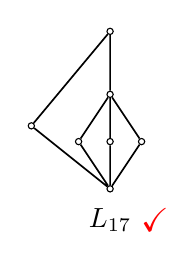
\begin{tikzpicture}[scale=.4]

          
        \node (bottom) at (0,0)  [draw, circle, inner sep=\dotsize] {};
        \node (top) at (0,5)  [draw, circle, inner sep=\dotsize] {};
        \node (n115) at (-1,1.5)  [draw, circle, inner sep=\dotsize] {};
        \node (015) at (0,1.5)  [draw, circle, inner sep=\dotsize] {};
        \node (115) at (1,1.5)  [draw, circle, inner sep=\dotsize] {};
        \node (n252) at (-2.5,2)  [draw, circle, inner sep=\dotsize] {};
        \node (03) at (0,3)  [draw, circle, inner sep=\dotsize] {};
        \draw[semithick] 
        (bottom) to (n252) to (top)
        (bottom) to (n115) to (03) to (115) to
        (bottom) to (015) to (03) to (top);
       %\draw (-4.5,2.2) node {$L \cong$};



          \draw (0,-1) node {$L_{17}$};
                {\color{red}\draw[font=\large] (1,-1) node{$\text{\rlap{$\checkmark$}}$ };}

        \end{tikzpicture}
      \end{center}
    \end{column}

    \begin{column}{0.2\textwidth}
      \begin{center}
        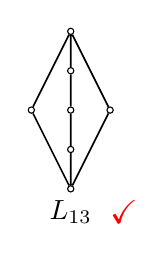
\begin{tikzpicture}[scale=.5]

          %\newcommand{\dotsize}{1};
\node (0) at (0,0) [draw, circle,inner sep=\dotsize] {};
\node (1) at (-0,1) [draw, circle, inner sep=\dotsize] {};
\node (2) at (1,2) [draw, circle, inner sep=\dotsize] {};
\node (3) at (-1,2) [draw, circle, inner sep=\dotsize] {};
\node (4) at (-0,2) [draw, circle, inner sep=\dotsize] {};
\node (5) at (-0,3) [draw, circle, inner sep=\dotsize] {};
\node (6) at (-0,4) [draw, circle, inner sep=\dotsize] {};
%\draw[font=\scriptsize] (0,-.5) node {[A4, (C2 x C2 x C2 x C2) : A5]};
%\draw[font=\scriptsize] (0,-1) node {SmallGroup(960,11358) Index 80};

\draw[semithick]
(0) to (1)
(0) to (2)
(0) to (3)
(1) to (4)
(2) to (6)
(3) to (6)
(4) to (5)
(5) to (6);

          \draw (0,-.6) node {$L_{13}$};
                {\color{red}\draw[font=\large] (1,-.6) node{$\text{\rlap{$\checkmark$}}$ };}

        \end{tikzpicture}
      \end{center}
    \end{column}

    \begin{column}{0.2\textwidth}
      \begin{center}
        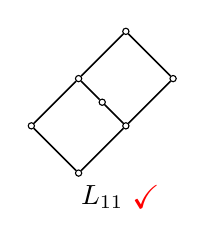
\begin{tikzpicture}[scale=.3]

          % L11 aka L3 
        \node (bottom) at (0,0)  [draw, circle, inner sep=\dotsize] {};
        \node (top) at (2,6)  [draw, circle, inner sep=\dotsize] {};
        \node (n22) at (-2,2)  [draw, circle, inner sep=\dotsize] {};
        \node (22) at (2,2)  [draw, circle, inner sep=\dotsize] {};
        \node (13) at (1,3)  [draw, circle, inner sep=\dotsize] {};
        \node (04) at (0,4)  [draw, circle, inner sep=\dotsize] {};
        \node (44) at (4,4)  [draw, circle, inner sep=\dotsize] {};

        \draw[semithick] (bottom) to (22) to (44) to (top) to (04) to (13) to (22)
        (bottom) to (n22) to (04);
  \draw (1,-1) node {$L_{11}$};
                {\color{red}\draw[font=\large] (2.3,-1) node { $\text{\rlap{$\checkmark$}}$};}

        \end{tikzpicture}
      \end{center}
    \end{column}

  \end{columns}


  \begin{columns}

    \begin{column}{0.2\textwidth}
      \begin{center}
        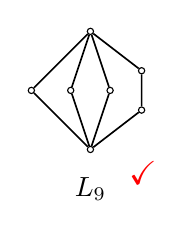
\begin{tikzpicture}[scale=.5]

          %% ``L9'' is the pentegon with two extra wings.
      \foreach \j in {0,3} 
      { \node (7\j) at (6.5,\j)  [draw, circle, inner sep=\dotsize] {};}
      \node (71) at (7,1.5)  [draw, circle, inner sep=\dotsize] {};
      \node (61) at (6,1.5)  [draw, circle, inner sep=\dotsize] {};
      \node (51) at (5,1.5)  [draw, circle, inner sep=\dotsize] {};
      \foreach \j in {1,2} 
      { \node (8\j) at (7.8,\j)  [draw, circle, inner sep=\dotsize] {};}
      \draw[semithick] (70) to (51) to (73) to (61) to (70) to (71) to (73) to
      (82) to (81) to (70);
      

          \draw (6.5,-1) node {$L_{9}$};
          \uncover<2->{
            {\color{red}\draw[font=\large] (7.5,-.6) node{$\text{\rlap{$\checkmark$}}$ };}
            %\draw[font=\large] (9.3,-.6) node { {\footnotesize Freese}};
          }
        \end{tikzpicture}
      \end{center}
    \end{column}


    \begin{column}{0.2\textwidth}
      \begin{center}
        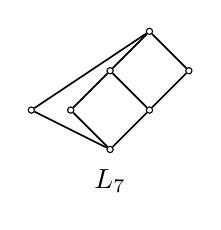
\begin{tikzpicture}[scale=.5]

          %%  The elusive winged-2x3 %%
      \node (01) at (0,1)  [draw, circle, inner sep=\dotsize] {};
      \foreach \j in {0,2} 
      { \node (1\j) at (1,\j)  [draw, circle, inner sep=\dotsize] {};}

      \foreach \j in {1,3} 
      { \node (2\j) at (2,\j)  [draw, circle, inner sep=\dotsize] {};}
      { \node (32) at (3,2)  [draw, circle, inner sep=\dotsize] {};}
      \draw[semithick] (10) to (01) to (12) to (23) to (32) to (21) to (10) (21) to (12);
      { \node (m11) at (-1,1)  [draw, circle, inner sep=\dotsize] {};}
      \draw[semithick] (10) to (m11) to (23);



%          \visible<3>{\node (18) at (1,1.3)  [draw, circle, red, inner sep=25pt] {};} 

          \draw (1,-.8) node {$L_7$};
        \end{tikzpicture}
      \end{center}
    \end{column}
  \end{columns}
\end{frame}









\begin{frame}[fragile,label=freese,shrink=5]{Contruction of an algebra $\bA$ with $\Con \bA \cong L_9$.}

  \begin{columns}
    \begin{column}{0.2\textwidth}

      \begin{center}
      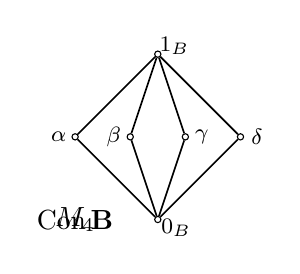
\begin{tikzpicture}[scale=.7]
                \node (250) at (2.5,0)  [draw, circle, inner sep=\dotsize] {};
        \node (253) at (2.5,3)  [draw, circle, inner sep=\dotsize] {};
        \foreach \i in {1,...,4} 
                 { 
                   \node (\i15) at (\i,1.5)  [draw, circle, inner sep=\dotsize] {};
                   \draw[semithick] (250) to (\i15) to (253);
                 }

        \uncover<2->{
          \draw[font=\footnotesize] 
          (0.7,1.5) node {$\alpha$} (1.7,1.5) node {$\beta$}
          (3.3,1.5) node {$\gamma$} (4.3,1.5) node {$\delta$}
          (2.8,3.15) node {$1_B$} (2.83,-.15) node {$0_B$};
        }
        \visible<1>{
          \draw  (1,0) node {$M_4$};}
        \visible<2->{
          \draw  (1,0) node {$\Con \bB$};}
      \end{tikzpicture}
      \end{center}

\vskip3mm

      \begin{center}
        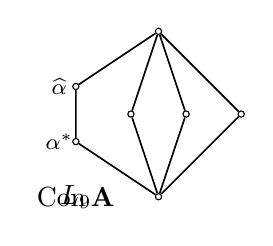
\begin{tikzpicture}[scale=.7]

                \node (70) at (6.5,0)  [draw, circle, inner sep=\dotsize] {};
      \node (71) at (7,1.5)  [draw, circle, inner sep=\dotsize] {};
      \node (73) at (6.5,3)  [draw, circle, inner sep=\dotsize] {};
      \node (61) at (6,1.5)  [draw, circle, inner sep=\dotsize] {};
      \node (51) at (5,1)  [draw, circle, inner sep=\dotsize] {};
      \node (52) at (5,2)  [draw, circle, inner sep=\dotsize] {};
      \node (81) at (8,1.5)  [draw, circle, inner sep=\dotsize] {};
      \draw[semithick] 
      (70) to (51) to (52) to (73)
      (70) to (61) to (73) 
      (70) to (71) to (73) 
      (70) to (81) to (73);

          \visible<1-3>{\draw  (5,0) node {$L_{9}$};}
          \visible<4->{\draw  (5,0) node {$\Con \bA$};}
          \visible<4->{\draw[font=\footnotesize] (4.7,2) node {$\widehat{\alpha}$} (4.7,1) node {$\alpha^*$};}

        \end{tikzpicture}
      \end{center}

    \end{column}


    \begin{column}{0.75\textwidth}
      \begin{enumerate}[Step 1]
      \item<2-> 
        Take a permutational algebra $\bB = \<B, F\>$ with congruence lattice $\Con\bB \cong M_4$.

        \vskip6pt
        
        \note{There are infinitely many, but apart from those involving 
          $S_3$, $C_3 \times C_3$, and $(C_3 \times C_3) \rtimes C_3$, they are quite
          large.  The next smallest G-set with $M_4$ congruence lattice that we
          know of comes from the group 
          $G = [ ( (C_3 \times C_3) \rtimes C_2 ) \times ( (C_3 \times C_3) \rtimes C_2 ) ] \rtimes C_2$
          acting on right cosets of $H \cong D_8$.  The index in this case is $|G:H| = 81$.
          (In \GAP, {\tt G:=SmallGroup(648,725)}.)}

        {\small
          \uncover<3->{\underline{Example:}
          \vskip4pt
          \begin{itemize}
%          \begin{itemize}[label=$\cdot$]
          \item
            Let $B = \{0, 1, \dots, 5\}$ index the elements of $S_3$ and
            consider the right regular action of $S_3$ on itself.
            \vskip5pt
          \item
            $g_0 = (0,4)(1,3)(2,5)$ and $g_1 = (0,1,2)(3,4,5)$ generate this
            action group, the image of $S_3 \hookrightarrow S_6$.
            \vskip5pt
          \item $\Con \<B , \{g_0, g_1\}\> \cong M_4$ with congruences
            \[
            \hskip-6mm            \alpha = | 0 1 2 | 3 4 5|, \; \beta = | 0 3 | 1 4 | 2 5 |, 
            \gamma = | 0 4|1 5| 2 3| , \; \delta = | 0 5|1 3| 2 4| .
            \]
          \end{itemize}}
        }

        \vskip6pt

\uncover<4->{
\hskip-10mm {\rmfamily {\bf Goal:} \emph{expand $\bB$ to an algebra $\bA$ that has
          $\alpha$ ``doubled'' in $\Con\bA$.}}}

        \vskip10pt

            \item<5-> Since $\alpha = \Cg^\bB(0,2)$, we let $A = B_0 \cup B_1 \cup B_2$ where
              \vskip-8pt
              \begin{align*}
                B_0 &= \{ {\color<5->{blue}0}, 1, {\color<5->{green}2}, 3, 4, 5\} = B\\
                B_1 &= \{{\color<5->{blue}0}, 6, 7, 8, 9, 10\}\\
                B_2 &= \{ 11, 12, {\color<5->{green}2}, 13, 14, 15\}.
              \end{align*}
            \item<6-> Define unary operations $e_0, e_1, e_2,\, s, \,g_0 e_0$, and $g_1 e_0$.
      \end{enumerate}

    \end{column}

  \end{columns}

\end{frame}

\begin{frame}[fragile,label=freese,shrink=5]{Contruction of an algebra $\bA$ with $\Con \bA \cong L_9$.}
  \begin{columns}

    \begin{column}{0.3\textwidth}
      \vskip2mm
      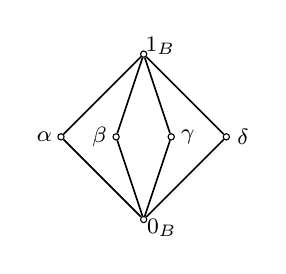
\begin{tikzpicture}[scale=.7]
                \node (250) at (2.5,0)  [draw, circle, inner sep=\dotsize] {};
        \node (253) at (2.5,3)  [draw, circle, inner sep=\dotsize] {};
        \foreach \i in {1,...,4} 
                 { 
                   \node (\i15) at (\i,1.5)  [draw, circle, inner sep=\dotsize] {};
                   \draw[semithick] (250) to (\i15) to (253);
                 }

        \draw[font=\footnotesize] 
        (0.7,1.5) node {$\alpha$} (1.7,1.5) node {$\beta$}
        (3.3,1.5) node {$\gamma$} (4.3,1.5) node {$\delta$}
        (2.8,3.15) node {$1_B$} (2.83,-.15) node {$0_B$};
      \end{tikzpicture}
    \end{column}

    \begin{column}{0.4\textwidth}
      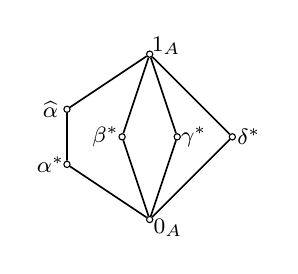
\begin{tikzpicture}[scale=.7]
              \node (70) at (6.5,0)  [draw, circle, inner sep=\dotsize] {};
      \node (71) at (7,1.5)  [draw, circle, inner sep=\dotsize] {};
      \node (73) at (6.5,3)  [draw, circle, inner sep=\dotsize] {};
      \node (61) at (6,1.5)  [draw, circle, inner sep=\dotsize] {};
      \node (51) at (5,1)  [draw, circle, inner sep=\dotsize] {};
      \node (52) at (5,2)  [draw, circle, inner sep=\dotsize] {};
      \node (81) at (8,1.5)  [draw, circle, inner sep=\dotsize] {};
      \draw[semithick] 
      (70) to (51) to (52) to (73)
      (70) to (61) to (73) 
      (70) to (71) to (73) 
      (70) to (81) to (73);

        \draw[font=\footnotesize] 
        (4.7,1) node {$\alpha^*$} (4.7,2) node {$\widehat{\alpha}$}
        (5.7,1.5) node {$\beta^*$} (7.3,1.5) node {$\gamma^*$} (8.3,1.5) node {$\delta^*$}
        (6.8,3.15) node {$1_A$} (6.83,-.15) node {$0_A$};
      \end{tikzpicture}
    \end{column}

  \end{columns}

  \begin{columns}
    \begin{column}{0.3\textwidth}
      \begin{center}
        $\Con \< B,\{g_0, g_1\}\>$

        \vskip-2pt
        \begin{align*}
          \alpha &= {\color<2->{blue}\pb 0, 1, 2 \pb 3, 4, 5\pb }\\[4pt]
          \beta &= {\color<2->{blue}\pb 0, 3 \pb  1, 4 \pb 2, 5 \pb} \\[3pt]
          \gamma &= {\color<2->{blue}\pb 0, 4\pb 1, 5\pb  2, 3\pb}  \\[3pt]
          \delta &= {\color<2->{blue}\pb 0, 5\pb 1, 3\pb  2, 4\pb} 
        \end{align*}
      \end{center}
    \end{column}

    \begin{column}{0.65\textwidth}
      \begin{center}
        $\Con \<A, F_A\>$
      \end{center}
      \begin{align*}
        \widehat{\alpha} &=|{\color<2->{blue}0,1,2},6,7,11,12|{\color<2->{blue}3,4,5}|8,9,10,13,14,15| \\
        \alpha^* &=|{\color<2->{blue}0,1,2},6,7,11,12|{\color<2->{blue}3,4,5}|8,9,10|13,14,15| \\[2pt]
        \beta^*&=|{\color<2->{blue}0,3},8|{\color<2->{blue}1,4}|{\color<2->{blue}2,5},15|6,9|7,10|11,13|12,14| \\[2pt]
        \gamma^*&=|{\color<2->{blue}0,4},9|{\color<2->{blue}1,5}|{\color<2->{blue}2,3},13|6,10|7,8|11,14|12,15| \\[2pt]
        \delta^*&=|{\color<2->{blue}0,5},10|{\color<2->{blue}1,3}|{\color<2->{blue}2,4},14|6,8|7,9,11,15|12,13|
      \end{align*}
    \end{column}
  \end{columns}

  \vskip4mm

  \only<2>{\[
    \alpha = \alpha^*\cap B^2 = \widehat{\alpha}\cap B^2,\; \quad
    \beta = \beta^*\cap B^2, \quad \dots %\quad \gamma = \gamma^*\cap B^2, \quad \delta = \delta^*\cap B^2.
    \]}

\end{frame}

\newcommand{\ifdot}{dotted}
%\newcommand{\ifdot}{dashed}
%\newcommand{\ifdot}{}

\begin{frame}[fragile,label=OA,shrink=5]{Why does it work?}
  \begin{columns}
    \begin{column}{0.3\textwidth}
      \begin{center}
        $\Con \< B,\{g_0, g_1\}\>$

        \vskip-2pt
        \begin{align*}
          \alpha &= |{\color<2,6,7>{blue}0, 1, 2} | {\color<2,6,7>{blue}3, 4, 5}|\\[4pt]
          \beta &= |{\color<3>{blue}0, 3} | {\color<3>{blue}1, 4} |{\color<3>{blue}2, 5} | \\[3pt]
          \gamma &= |{\color<4>{blue}0, 4}|{\color<4>{blue}1, 5}|{\color<4>{blue}2, 3}| \\[3pt]
          \delta &= |{\color<5>{blue}0, 5}|{\color<5>{blue}1, 3}|{\color<5>{blue} 2, 4}| 
        \end{align*}
      \end{center}
    \end{column}

    \begin{column}{0.4\textwidth}
      {
        \begin{tikzpicture}[scale=.7]

          \visible<1-48,62->{ % B_0
            \foreach \j in {0,1,2} {
              \draw (\j -1, 0.5) node {$\j$};
              \pgfmathtruncatemacro{\x}{\j+3}
              \draw (\j -1, -0.5) node {$\x$};
            }
            \draw (0,-1.5) node {$B_0$};
          }

          \visible<2,6>{ % alpha
            \draw[rounded corners,\ifdot] (-1.3,-.8) rectangle (1.3,-.2);
            \draw[rounded corners,\ifdot] (-1.3,.8) rectangle (1.3,.2);
            \draw[font=\Large] (-2,-1) node {$\alpha$};
          }
          \visible<3>{  % beta
            \draw[rounded corners,\ifdot] (-1.3,-.8) rectangle (-.7,.8);
            \draw[rounded corners,\ifdot] (-.3,-.8) rectangle (.3,.8);
            \draw[rounded corners,\ifdot] (1.3,-.8) rectangle (.7,.8);
            \draw[font=\Large] (-2,-1) node {$\beta$};
          }
          \visible<4>{   % beta
            \draw[rounded corners,\ifdot] (1,-.85) to (1.35,-.5) to  (-0,.85) to (-.35,.5) to (1,-.85);
            \draw[rounded corners,\ifdot] (0,-.85) to (0.35,-.5) to  (-1,.85) to (-1.35,.5) to (0,-.85);
            \draw[rounded corners,\ifdot] (.8,.05) to (1.37,.35) to  (1.1,.87) to (.4,.4);
            \draw[rounded corners,\ifdot] (-.8,-.05) to (-1.37,-.35) to  (-1.1,-.87) to (-.4,-.4);
            \draw[\ifdot] (-0.1,.2) to (-.28,.13);
            \draw[\ifdot] (0.1,-.2) to (.28,-.13);
            \draw[font=\Large] (-2,-1) node {$\gamma$};
          }

          \visible<5>{ % delta
            \draw[rounded corners,\ifdot] (-1,-.85) to (-1.35,-.5) to  (0,.85) to (.35,.5) to (-1,-.85);
            \draw[rounded corners,\ifdot] (0,-.85) to (-0.35,-.5) to  (1,.85) to (1.35,.5) to (0,-.85);
            \draw[rounded corners,\ifdot] (-.8,.05) to (-1.37,.35) to  (-1.1,.87) to (-.4,.4);
            \draw[rounded corners,\ifdot] (.8,-.05) to (1.37,-.35) to  (1.1,-.87) to (.4,-.4);
            \draw[\ifdot] (0.1,.2) to (.28,.13);
            \draw[\ifdot] (-0.1,-.2) to (-.28,-.13);
            \draw[font=\Large] (-2,-1) node {$\delta$};
          }

          %% B0 rectangle %%
          \visible<8-34>{\draw[rounded corners,blue] (-1.5,-1) rectangle (1.5,1); }
          \visible<1-7,35-48,62->{\draw[rounded corners,dotted] (-1.5,-1) rectangle (1.5,1);}

          %% B1 %%
          \visible<7,35->{ 
            \foreach \j in {0,1,2} {
              \pgfmathtruncatemacro{\x}{10-\j}
              \draw (\j -3, 1.5) node {$\x$};
            }
            \draw (-3, .5) node {$7$} (-2, .5) node {$6$}; 
          }
          \visible<7,8,35->{\draw  (-2,2.5) node {$B_1$};}
          \visible<7,62->{\draw[rounded corners,dotted] (-3.5,0) rectangle (-0.5,2);}
          \visible<35-61>{\draw[rounded corners,blue] (-3.5,0) rectangle (-0.5,2);}
          \visible<49-61>{\draw (-1, .5) node {$0$}; }

          %% B2 %%
          \visible<7-21,62->{ 
            {\color<9-21>{gray}
              \foreach \j in {0,1,2} {
                \pgfmathtruncatemacro{\y}{15-\j}
                \draw (\j +1, 1.5) node {$\y$};
              }
              \draw (3, .5) node {$11$} (2, .5) node {$12$};
            }
          }
          \visible<7-22,35,62->{\draw  (2,2.5) node {$B_2$};}
          \visible<7-21,62->{\draw[rounded corners,dotted] (3.5,0) rectangle (0.5,2);}

          \foreach \i in {0,...,11}{
            \pgfmathtruncatemacro{\v}{\i+8}
            \visible<\v>{ 
              {\color<18-19>{gray}
                \eImageOfBOne{\i}}
            }
          }
          \foreach \i in {0,...,11}{
            \pgfmathtruncatemacro{\v}{\i+22}
            \visible<\v>{ 
              {\color<32-33>{gray}
                \eImageOfBTwo{\i}
              }
            }
          }

          \foreach \i in {0,...,11}{
            \pgfmathtruncatemacro{\v}{\i+35}
            \visible<\v>{ 
              {\color<46-47>{gray}
                \eImageOfBTwo{\i}
              }
            }
          }

        %% Rotate B0 onto B1 %%
        \foreach \i in {0,1,...,11}{
          \pgfmathtruncatemacro{\v}{\i+49}
          \visible<\v>{ 
            {\color<60-61>{gray}
              \eImageOfBZero{\i}       %% use -\i for clockwise rotation
            }
          }
        }

        \end{tikzpicture}
      }
    \end{column}
  \end{columns}
  \begin{columns}
    \begin{column}{0.3\textwidth}
      \begin{itemize}
      \item<7-> $A = B_0 \cup B_1 \cup B_2$
        \vskip4pt
      \item<8->Unary operations 
        \begin{align*}
          \alt<8-34>{{\color{blue} e_0} & {\color{blue} : A \twoheadrightarrow B_0 }}
                    {{\color{gray} e_0} & {\color{gray} : A \twoheadrightarrow B_0 }}\\
          \alt<35-61>{{\color{blue} e_1} &{\color{blue} : A \twoheadrightarrow B_1}}
                     {{\color{gray} e_1} &{\color{gray} : A \twoheadrightarrow B_1}}\\
          {\color{gray} e_2} &{\color{gray} : A \twoheadrightarrow B_2}\\
          \alt<62>{{\color{blue} s} &{\color{blue} : A \twoheadrightarrow B_0}}
                  {{\color{gray} s} &{\color{gray} : A \twoheadrightarrow B_0}}\\
        \end{align*}
        \[
        \alt<63>{{\color{blue} g e_0} {\color{blue} : A \stackrel{e_0}{\twoheadrightarrow} B_0 \stackrel{g}{\rightarrow} B_0}}
                {{\color{gray} g e_0} {\color{gray} : A \stackrel{e_0}{\twoheadrightarrow} B_0 \stackrel{g}{\rightarrow} B_0}}
        \]
      \end{itemize}
    \end{column}
    \begin{column}{0.5\textwidth}
      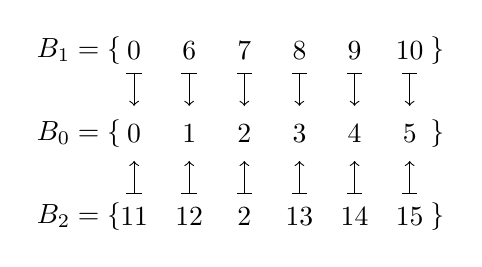
\begin{tikzpicture}[scale=.7]

        \visible<6->{                      
          
          %%% B_0 %%%
          \draw (-1,0) node {$B_0 = \{$};
          \foreach \i in { 0, 1, 2, 3, 4, 5}{ 
            \draw (\i,0) node {$\i$}; 
            \visible<8,9,12,13,16,17,20,21-34>{ \draw [|->] (\i,1.1) -- (\i,0.5);}
            \visible<8-23,26-28,31-34>{ \draw [|->] (\i,-1.1) -- (\i,-0.5); }
          }
          \draw (5.5,0) node {$\}$};
        }
        
        \visible<7->{                                               

          %%% B_1 %%%
          \draw (-1,1.5) node {$B_1 =\{$} (0,1.5) node {$0$};
          \foreach \i in { 6, 7, 8, 9, 10}{ \draw (\i-5,1.5) node {$\i$}; }
          \draw (5.5,1.5) node {$\}$};
          
          %%% B_2 %%%
          \draw (-1,-1.5) node {$B_2 =\{$} (0,-1.5) node {$11$} (1,-1.5) node {$12$} (2,-1.5) node {$2$};
          \foreach \i in { 13, 14, 15}{ \draw (\i-10,-1.5) node {$\i$}; }
          \draw (5.5,-1.5) node {$\}$};
        }

      \end{tikzpicture}
    \end{column}

  \end{columns}
\end{frame}





\begin{frame}[fragile,label=OAop3,shrink=5]{Why does it work?}

  \begin{columns}
    \begin{column}{0.3\textwidth}
      \begin{center}
        $\Con \< B,\{g_0, g_1\}\>$

        \vskip-2pt
        \begin{align*}
          \alpha &= |0, 1, 2 | 3, 4, 5|\\[4pt]
          \beta &= |0, 3 | 1, 4 |2, 5 | \\[3pt]
          \gamma &= |0, 4| 1, 5|2, 3| \\[3pt]
          \delta &= |0, 5|1, 3|2, 4| 
        \end{align*}
      \end{center}
    \end{column}

    \begin{column}{0.3\textwidth}
      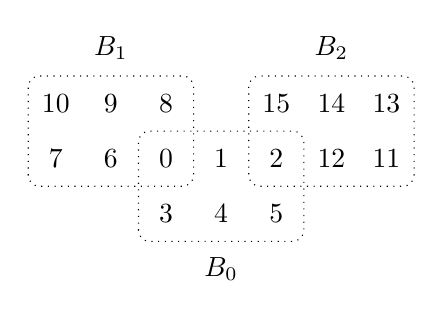
\begin{tikzpicture}[scale=.7]

        %% B0 %%
        \foreach \j in {0,1,2} {
          \draw (\j -1, 0.5) node {$\j$};
          \pgfmathtruncatemacro{\x}{\j+3}
          \draw (\j -1, -0.5) node {$\x$};
        }
        \draw (0,-1.5) node {$B_0$};
        \draw[rounded corners,dotted] (-1.5,-1) rectangle (1.5,1);

        %% B1 %%
        \foreach \j in {0,1,2} {
          \pgfmathtruncatemacro{\x}{10-\j}
          \draw (\j -3, 1.5) node {$\x$};
        }
        \draw (-3, .5) node {$7$} (-2, .5) node {$6$}; 
        \draw[rounded corners,dotted] (-3.5,0) rectangle (-0.5,2);
        \draw  (-2,2.5) node {$B_1$};

        %% B2 %%
        \foreach \j in {0,1,2} {
          \pgfmathtruncatemacro{\y}{15-\j}
          \draw (\j +1, 1.5) node {$\y$};
        }
        \draw (3, .5) node {$11$} (2, .5) node {$12$};
        \draw  (2,2.5) node {$B_2$};
        \draw[rounded corners,dotted] (3.5,0) rectangle (0.5,2);


      \end{tikzpicture}
    \end{column}
  \end{columns}
  \begin{columns}
    \begin{column}{0.3\textwidth}
      \begin{itemize}
      \item $A = B_0 \cup B_1 \cup B_2$
        \vskip4pt
      \item Unary operations 
        \begin{align*}
          {\color{gray} e_0} & {\color{gray} : A \twoheadrightarrow B_0 } \\
          {\color{gray} e_1} &{\color{gray} : A \twoheadrightarrow B_1}\\
          {\color{gray} e_2} &{\color{gray} : A \twoheadrightarrow B_2}\\
          {\color{blue} s} &{\color{blue} : A \twoheadrightarrow B_0}
        \end{align*}
        \[
          {\color{gray} g e_0} {\color{gray} : A \stackrel{e_0}{\twoheadrightarrow} B_0 \stackrel{g}{\rightarrow} B_0}
          \]
      \end{itemize}
    \end{column}
    \begin{column}{0.5\textwidth}
      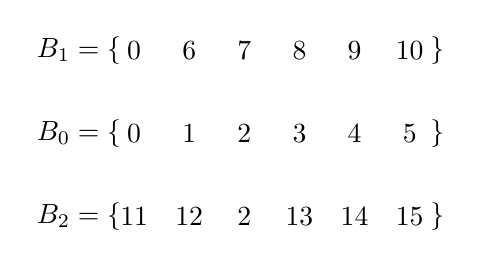
\begin{tikzpicture}[scale=.7]

        %%% B_0 %%%
        \draw (-1,0) node {$B_0 = \{$};
        \foreach \i in { 0, 1, 2, 3, 4, 5}{ 
          \draw (\i,0) node {$\i$}; 
        }
        \draw (5.5,0) node {$\}$};

        %%% B_1 %%%
        \draw (-1,1.5) node {$B_1 =\{$} (0,1.5) node {$0$};
        \foreach \i in { 6, 7, 8, 9, 10}{ \draw (\i-5,1.5) node {$\i$}; }
        \draw (5.5,1.5) node {$\}$};
        
        %%% B_2 %%%
        \draw (-1,-1.5) node {$B_2 =\{$} (0,-1.5) node {$11$} (1,-1.5) node {$12$} (2,-1.5) node {$2$};
        \foreach \i in { 13, 14, 15}{ \draw (\i-10,-1.5) node {$\i$}; }
        \draw (5.5,-1.5) node {$\}$};


      \end{tikzpicture}
    \end{column}

  \end{columns}
\end{frame}



\renewcommand{\ifdot}{dotted}
\begin{frame}[fragile,label=OAcong,shrink=5]{Why does it work?}

  \begin{columns}
    \begin{column}{0.3\textwidth}
      \begin{center}
        $\Con \< B,\{g_0, g_1\}\>$

        \vskip-2pt
        \begin{align*}
          \alpha &= {\color<2>{blue} \pb 0, 1, 2 \pb 3, 4, 5\pb }\\[4pt]
          \beta &= {\color<5>{blue} \pb 0, 3 \pb 1, 4 \pb 2, 5 \pb} \\[3pt]
          \gamma &= |0, 4| 1, 5|2, 3| \\[3pt]
          \delta &= |0, 5|1, 3|2, 4| 
        \end{align*}
      \end{center}
    \end{column}

    \begin{column}{0.3\textwidth}
      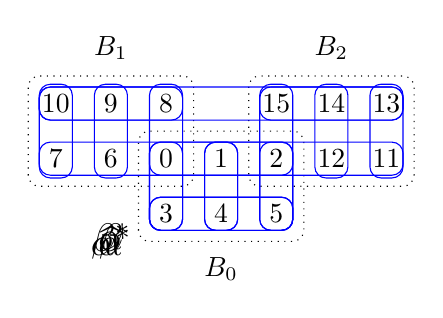
\begin{tikzpicture}[scale=.7]

        %% B0 %%
        \foreach \j in {0,1,2} {
          \draw (\j -1, 0.5) node {$\j$};
          \pgfmathtruncatemacro{\x}{\j+3}
          \draw (\j -1, -0.5) node {$\x$};
        }
        \draw (0,-1.5) node {$B_0$};
        \draw[rounded corners,dotted] (-1.5,-1) rectangle (1.5,1);

        %% B1 %%
        \foreach \j in {0,1,2} {
          \pgfmathtruncatemacro{\x}{10-\j}
          \draw (\j -3, 1.5) node {$\x$};
        }
        \draw (-3, .5) node {$7$} (-2, .5) node {$6$}; 
        \draw[rounded corners,dotted] (-3.5,0) rectangle (-0.5,2);
        \draw  (-2,2.5) node {$B_1$};

        %% B2 %%
        \foreach \j in {0,1,2} {
          \pgfmathtruncatemacro{\y}{15-\j}
          \draw (\j +1, 1.5) node {$\y$};
        }
        \draw (3, .5) node {$11$} (2, .5) node {$12$};
        \draw  (2,2.5) node {$B_2$};
        \draw[rounded corners,dotted] (3.5,0) rectangle (0.5,2);

        \visible<2>{ % alpha
          \draw[rounded corners,blue] (-1.3,-.8) rectangle (1.3,-.2);
          \draw[rounded corners,blue] (-1.3,.8) rectangle (1.3,.2);
          \draw[font=\Large] (-2,-1) node {$\alpha$};
        }
        \visible<3,4>{ % \alpha^*
          % B0 lower rectangle
          \draw[rounded corners,blue] (-1.3,-.8) rectangle (1.3,-.2);
          % long rectangle
          \draw[rounded corners,blue] (-3.3,.8) rectangle (3.3,.2); 
        }
        \visible<3>{ % \alpha^*
          \draw[rounded corners,blue] (-3.3,1.2) rectangle (-.7,1.8);  
          \draw[rounded corners,blue] (3.3,1.2) rectangle (.7,1.8); 
          \draw[font=\Large] (-2,-1) node {$\alpha^*$};
        }
        \visible<4>{ % \widehat{\alpha}
          \draw[rounded corners,blue] (-3.3,1.2) rectangle (3.3,1.8);  
          \draw[font=\Large] (-2,-1) node {$\widehat{\alpha}$};
        }
        \visible<5>{  % beta
          \draw[rounded corners,blue] (-1.3,-.8) rectangle (-.7,.8);
          \draw[rounded corners,blue] (-.3,-.8) rectangle (.3,.8);
          \draw[rounded corners,blue] (1.3,-.8) rectangle (.7,.8);
          \draw[font=\Large] (-2,-1) node {$\beta$};
        }
        \visible<6->{  % beta
          \draw[rounded corners,blue] (-1.3,-.8) rectangle (-.7,1.85);  % big left rect
          \draw[rounded corners,blue] (-.3,-.8) rectangle (.3,.8);
          \draw[rounded corners,blue] (1.3,-.8) rectangle (.7,1.85);  % big right rect
          \draw[rounded corners,blue] (-1.7,.15) rectangle (-2.3,1.85);
          \draw[rounded corners,blue] (-2.7,.15) rectangle (-3.3,1.85);  % small B1 far left
          \draw[rounded corners,blue] (1.7,.15) rectangle (2.3,1.85);
          \draw[rounded corners,blue] (2.7,.15) rectangle (3.3,1.85); % small B2 far right
          \draw[font=\Large] (-2,-1) node {$\beta^*$};
        }

      \end{tikzpicture}
    \end{column}
  \end{columns}
  \begin{columns}
    \begin{column}{0.3\textwidth}
      \visible<7>{\emph{Why don't the $\beta$ classes of $B_1$ and $B_2$ mix?}}
    \end{column}
    \begin{column}{0.5\textwidth}
      \begin{center}
        $\Con \<A, F_A\>$
      \end{center}
      \begin{align*}
        \widehat{\alpha} &= {\color<4>{blue} \pb 0,1,2,6,7,11,12\pb 3,4,5 \pb 8,9,10,13,14,15\pb } \\
        \alpha^* &= {\color<3>{blue} \pb  0,1,2,6,7,11,12 \pb 3,4,5 \pb 8,9,10 \pb 13,14,15 \pb}  \\[2pt]
        \beta^*&= {\color<6->{blue} \pb 0,3,8 \pb 1,4 \pb 2,5,15 \pb 6,9 \pb 7,10 \pb 11,13 \pb 12,14 \pb } \\[2pt]
        \gamma^*&= \pb 0,4,9 \pb 1,5 \pb 2,3,13 \pb 6,10 \pb 7,8 \pb 11,14 \pb 12,15 \pb  \\[2pt]
        \delta^*&= \pb 0,5,10 \pb 1,3 \pb 2,4,14 \pb 6,8 \pb 7,9,11,15 \pb 12,13 \pb 
      \end{align*}
    \end{column}

  \end{columns}
\end{frame}

\begin{frame}[fragile,label=OAEx2,shrink=5]{Variations on the same example... }

  \begin{columns}
    \begin{column}{0.7\textwidth}
      \begin{itemize}
      \item 
        Suppose we want $\beta = \Cg^\bB(0,3) =| 0, 3 | 2, 5 | 1, 4 |$ to 
        \vskip4pt
        have non-trivial inverse image $\beta\resB^{-1} = [\beta^*, \widehat{\beta}]$.  
        \vskip6pt
      \item<2-> Select elements 0 and 3 as intersection points:
        \[
        A = B_0 \cup B_1 \cup B_2 \quad \text{where}
        \]
        \begin{align*}
          B_0 &= \{{\color{blue} 0}, 1,  2,  {\color{green}3},  4,  5\}\\
          B_1 &= \{{\color{blue} 0}, 6,  7,  8,  9, 10\}\\
          B_2 &= \{11, 12, 13, {\color{green}3}, 14, 15\}.
        \end{align*}
      \end{itemize}
    \end{column}
    \begin{column}{0.3\textwidth}
      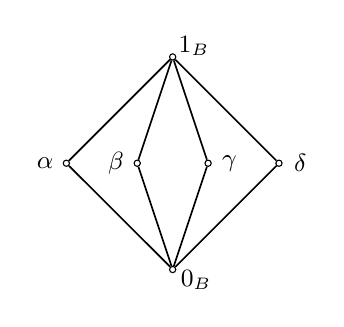
\begin{tikzpicture}[scale=.9]
                \node (250) at (2.5,0)  [draw, circle, inner sep=\dotsize] {};
        \node (253) at (2.5,3)  [draw, circle, inner sep=\dotsize] {};
        \foreach \i in {1,...,4} 
                 { 
                   \node (\i15) at (\i,1.5)  [draw, circle, inner sep=\dotsize] {};
                   \draw[semithick] (250) to (\i15) to (253);
                 }

        \draw[font=\small] 
        (0.7,1.5) node {$\alpha$} (1.7,1.5) node {$\beta$}
        (3.3,1.5) node {$\gamma$} (4.3,1.5) node {$\delta$}
        (2.8,3.15) node {$1_B$} (2.83,-.15) node {$0_B$};
      \end{tikzpicture}

    \end{column}

  \end{columns}

  \vskip-5mm

  \begin{columns}
    \begin{column}{0.3\textwidth}

      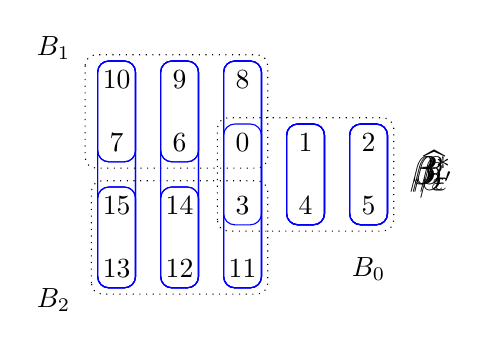
\begin{tikzpicture}[scale=.8]

        %% B0 %%
        \foreach \j in {0,1,2} {
          \draw (\j -1, 0.5) node {$\j$};
          \pgfmathtruncatemacro{\x}{\j+3}
          \draw (\j -1, -0.5) node {$\x$};
        }
        \draw (1,-1.5) node {$B_0$};
        \draw[rounded corners,dotted] (-1.4,-.9) rectangle (1.4,.9);

        \visible<3->{

          %% B1 %%
          \foreach \j in {0,1,2} {
            \pgfmathtruncatemacro{\x}{10-\j}
            \draw (\j -3, 1.5) node {$\x$};
          }
          \draw (-3, .5) node {$7$} (-2, .5) node {$6$}; 
          \draw[rounded corners,dotted] (-3.5,1.9) rectangle (-0.6,.1);
          \draw  (-4,2) node {$B_1$};

          %% B2 %%
          \foreach \j in {0,1,2} {
            \pgfmathtruncatemacro{\y}{13-\j}
            \draw (\j -3, -1.5) node {$\y$};
          }
          \draw (-3, -.5) node {$15$} (-2, -.5) node {$14$};
          \draw  (-4,-2) node {$B_2$};
          \draw[rounded corners,dotted] (-3.4,-1.9) rectangle (-0.6,-.1);
        }

        \visible<1-3>{  % beta
          \draw[rounded corners,blue] (-1.3,-.8) rectangle (-.7,.8);
          \draw[rounded corners,blue] (-.3,-.8) rectangle (.3,.8);
          \draw[rounded corners,blue] (1.3,-.8) rectangle (.7,.8);
          \draw[font=\Large] (2,0) node {$\beta$};
        }
        \visible<4>{  % beta^*
          \draw[rounded corners,blue] (-1.3,-1.8) rectangle (-.7,1.8);  % big rect
          \draw[rounded corners,blue] (-.3,-.8) rectangle (.3,.8);
          \draw[rounded corners,blue] (.7,-.8) rectangle (1.3,.8);     % right rect
          \draw[rounded corners,blue] (-1.7,.2) rectangle (-2.3,1.8);  % small B1 middle
          \draw[rounded corners,blue] (-2.7,.2) rectangle (-3.3,1.8);  % small B1 left
          \draw[rounded corners,blue] (-1.7,-.2) rectangle (-2.3,-1.8);% small B2 middle 
          \draw[rounded corners,blue] (-2.7,-.2) rectangle (-3.3,-1.8);% small B2 far left
          \draw[font=\Large] (2,0) node {$\beta^*$};
        }
        \visible<5>{  % \widehat{\beta}
          \draw[rounded corners,blue] (-1.3,-1.8) rectangle (-.7,1.8);  % big B0 rect
          \draw[rounded corners,blue] (-.3,-.8) rectangle (.3,.8);        % middle B0 rect
          \draw[rounded corners,blue] (.7,-.8) rectangle (1.3,.8);        % right B0 rect
          \draw[rounded corners,blue] (-3.3,-1.8) rectangle (-2.7,1.8);    % large far left
          \draw[rounded corners,blue] (-2.3,-1.8) rectangle (-1.7,1.8);  % small B2 far left
          \draw[font=\Large] (2,0) node {$\widehat{\beta}$};
        }
        \visible<6>{  % beta\eps1
          \draw[rounded corners,blue] (-1.3,-1.8) rectangle (-.7,1.8); % big rect
          \draw[rounded corners,blue] (-.3,-.8) rectangle (.3,.8);     % middle B0 rect
          \draw[rounded corners,blue] (.7,-.8) rectangle (1.3,.8);     % right rect
          \draw[rounded corners,blue] (-2.7,.2) rectangle (-3.3,1.8);  % small B1 left
          \draw[rounded corners,blue] (-1.7,1.8) rectangle (-2.3,-1.8);% big B1B2 middle 
          \draw[rounded corners,blue] (-2.7,-.2) rectangle (-3.3,-1.8);% small B2 far left
          \draw[font=\Large] (2,0) node {$\beta_\eps$};
        }
        \visible<7->{  % beta\eps2
          \draw[rounded corners,blue] (-1.3,-1.8) rectangle (-.7,1.8); % big rect
          \draw[rounded corners,blue] (-.3,-.8) rectangle (.3,.8);     % middle B0 rect
          \draw[rounded corners,blue] (.7,-.8) rectangle (1.3,.8);     % right rect
          \draw[rounded corners,blue] (-1.7,.2) rectangle (-2.3,1.8);  % small B1 middle
          \draw[rounded corners,blue] (-1.7,-.2) rectangle (-2.3,-1.8);% small B2 middle 
          \draw[rounded corners,blue] (-2.7,1.8) rectangle (-3.3,-1.8);%  big B1/B2 left
          \draw[font=\Large] (2,0) node {$\beta_{\eps'}$};
        }

      \end{tikzpicture}

    \end{column}

    \newcommand{\bigdotsize}{1.5pt}
    \begin{column}{0.3\textwidth}
      \centering
      \visible<4->{
        \begin{tikzpicture}[scale=1]
          \node (bottom) at (6.5,0)  [draw, circle, inner sep=\dotsize] {};  % bottom
          \node (71) at (7,1.5)  [draw, circle, inner sep=\dotsize] {};  % delta
          \node (top) at (6.5,3)  [draw, circle, inner sep=\dotsize] {}; % top
          \alt<4>{\node (61) at (6.1,1)  [fill, circle, red, inner sep=\bigdotsize] {};}  % beta^*}
                 {\node (61) at (6.1,1)  [draw, circle, inner sep=\dotsize] {};}  
                 \alt<5>{\node (62) at (6.1,2)  [fill, circle, red, inner sep=\bigdotsize] {};}  % hat{beta}
                        {\node (62) at (6.1,2)  [draw, circle, inner sep=\dotsize] {};}  % hat{beta}
                        \visible<6>{\node (63) at (5.7,1.5)  [fill, circle, red, inner sep=\bigdotsize] {};} % beta\eps
                        \visible<7->{\node (63) at (5.7,1.5)  [fill, circle, inner sep=\dotsize] {};} % beta\eps
                        \visible<7>{\node (64) at (6.5,1.5)  [fill, circle, red, inner sep=\bigdotsize] {};} % beta\eps'
                        \visible<8->{\node (64) at (6.5,1.5)  [fill, circle, inner sep=\dotsize] {};} % beta\eps'
                        \node (51) at (5,1.5)  [draw, circle, inner sep=\dotsize] {};  % alpha
                        \node (81) at (8,1.5)  [draw, circle, inner sep=\dotsize] {};
                        \draw[semithick] 
                        (bottom) to (51) to (top) to (62)
                        (bottom) to (61) 
                        (bottom) to (71) to (top) 
                        (bottom) to (81) to (top);
                        \visible<4-5>{\draw[dotted,semithick] (61) to (62);}
                        \visible<6->{\draw[semithick] (61) to (63) to (62);}
                        \visible<7->{\draw[semithick] (61) to (64) to (62);}
                        \draw (4.8,1.5) node {$\alpha^*$};
                        \draw (5.98,2.12) node {$\widehat{\beta}$};
                        \visible<6->{\draw (5.55,1.4) node {$\beta_\eps$};}
                        \visible<7->{\draw (6.65,1.3) node {$\beta_{\eps'}$};}
                        \draw (6,.8) node {$\beta^*$};
                        \draw (7.25,1.5) node {$\gamma^*$};
                        \draw (8.2,1.5) node {$\delta^*$};
                        \draw (6.7,3.15) node {$1_A$};
                        \draw (6.73,-.15) node {$0_A$};
        \end{tikzpicture}
      }
    \end{column}
  \end{columns}
\end{frame}


\begin{frame}[fragile,label=PAP,shrink=5]{The $P^5$ Lemma}
  \begin{lemma}[\PAP]
    Let $\bA = \langle A, F\rangle$ be a unary algebra with 
    %$F$ a monoid, 
    $e^2=e\in F$.\\[4pt]
    Define $\bB = \langle B, G\rangle$ with
    \[
    B= e(A) \quad \text{ and } \quad G = \{ef\rvert_B : f\in F\}.
    \]
    Then 
    \[
    \Con \bA \ni \theta \mapsto \theta \cap B^2 \in \Con \bB
    \]
    is a lattice epimorphism.
  \end{lemma}
  %% \uncover<2->{
  %% McKenzie (1980?) introduced the mapping $\hatmap$ defined on $\Con\bB$ by
  %% \[
  %% \widehat{\beta} = \{(x,y) \in A^2 : (ef(x), ef(y))\in \beta\, \text{ for all }\, f\in \Pol_1(\bA) \}.
  %% \]
  %% Clearly, $\hatmap : \Con\bB \rightarrow \Con\bA$.
  %% }
\end{frame}


\begin{frame}[fragile,label=PAP1,shrink=5]{Residuation Lemma}  %The maps $\resB$, $^*$, and $\hatmap$.}
\vskip3mm

  \begin{itemize}
  \item Define $\hatmap : \Con\bB \rightarrow \Con\bA$ by %(McKenzie, 1980) %$\hatmap$ defined on $\Con\bB$ by
    \[
    \widehat{\beta} = \{(x,y) \in A^2 : (ef(x), ef(y))\in \beta\, \text{ for all }\, f\in \Pol_1(\bA) \}.
    \]
    %% \vskip-4pt
    %%     \begin{itemize}
    %%     \item<2-> Note that $\hatmap : \Con\bB \rightarrow \Con\bA$. 
    %%     \end{itemize}
    %% For example, if $(x,y) \in \widehat{\beta}$ and $g\in \Pol_1(\bA)$, then for all $f\in \Pol_1(\bA)$ we
    %% have $(efg(x),efg(y)) \in \beta$, so $(g(x),g(y))\in \widehat{\beta}$.
  \item<2->
    For each $\beta \in \Con\bB$, let $\beta^* = \Cg^\bA(\beta)$.  That is,
    \[
    ^*: \Con\bB \rightarrow \Con\bA
    \]
    is the congruence generation operator restricted to $\Con\bB$.
  \end{itemize}
  \uncover<3->{
    \begin{lemma}
      ~
      \begin{enumerate}[(i)]
      \item $^*: \Con\bB \rightarrow \Con\bA$ is a residuated mapping with
        residual $\resB$.
        \vskip6pt
      \item $\resB : \Con\bA \rightarrow \Con\bB$ is a residuated mapping with
        residual $\hatmap$.
        \vskip6pt
      \item For all $\alpha \in \Con\bA, \, \beta \in \Con\bB$,
        \[
        \beta = \alpha\resB \quad \Leftrightarrow  \quad 
        \beta^* \leq \alpha \leq \widehat{\beta}.
        \]
        In particular, 
        $\beta^*\resB = \beta = \widehat{\beta}\resB$.
      \end{enumerate}
    \end{lemma}
  }
\end{frame}

\begin{frame}[fragile,label=OAresults,shrink=5]{The structure of the interval $[\beta^*, \hbeta]\leq \bCon \bA$.}

\vskip2mm

  \begin{itemize}
  \item If $\beta \in \Con \bB$ is a coatom of $\bCon \bB$ with $m$ congruence classes then
        the interval $[\beta^*, \hbeta]$ in $\bCon \bA$ is $\two^{m-1}$.
  \end{itemize}

  \begin{columns}
    \begin{column}{0.3\textwidth}

      {\scalefont{.8}
        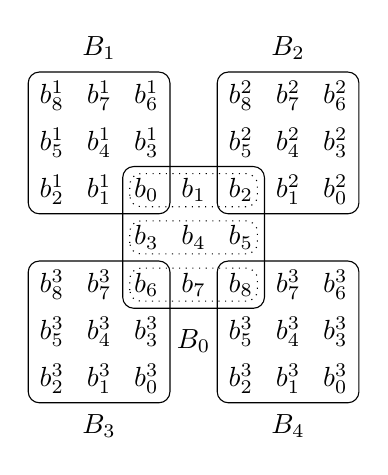
\begin{tikzpicture}[scale=.6]
          \draw[rounded corners] (-1.5,-1.5) rectangle (1.5,1.5);
          \draw[rounded corners] (.5,.5) rectangle (3.5,3.5);
          \visible<2->{\draw[rounded corners] (.5,-3.5) rectangle (3.5,-.5) (-3.5,-3.5) rectangle (-.5,-.5);}
          \draw[rounded corners] (-3.5,.5) rectangle (-.5,3.5);
          \draw[rounded corners, dotted] (-1.35,.65) rectangle (1.35,1.35);  
          \draw[rounded corners, dotted] (-1.35,-.35) rectangle (1.35,.35);
          \draw[rounded corners, dotted] (-1.35,-1.35) rectangle (1.35,-.65);

          \draw (0,-2.2) node {$B_0 $};
          %%    % B1
          \draw (-2, 4) node {$B_1$};
          \draw (-1, 1) node {$b_0$};
          \foreach \i in {0,1,2} {
            \foreach \j in {1,2} {
              \pgfmathtruncatemacro{\x}{3*\i+\j}
              \draw (-\j - 1, \i + 1) node {$b^1_\x$};
            }
          }
          \foreach \i in {1,2} {
            \foreach \j in {0} {
              \pgfmathtruncatemacro{\x}{3*\i+\j}
              \draw (-\j - 1, \i + 1) node {$b^1_\x$};
            }
          }
          \draw (0, 1) node {$b_1$};

          %%    % B2
          \draw (2, 4) node {$B_2$};
          \draw (1, 1) node {$b_2$};
          \foreach \i in {0,1,2} {
            \foreach \j in {1,2} {
              \pgfmathtruncatemacro{\x}{3*\i+(2-\j)}
              \draw (\j + 1, \i + 1) node {$b^2_\x$};
            }
          }
          \foreach \i in {1,2} {
            \foreach \j in {0} {
              \pgfmathtruncatemacro{\x}{3*\i+(2-\j)}
              \draw (\j + 1, \i + 1) node {$b^2_\x$};
            }
          }
          \foreach \j in {3,4,5} {
            \draw (\j -4, 0) node {$b_\j$};
          }

          \foreach \j in {6,7,8} {
            \draw (\j -7, -1) node {$b_\j$};
          }
          \visible<2->{
            %%    % B3
            \draw (-2, -4) node {$B_3$};

            \foreach \i in {0,1,2} {
              \foreach \j in {1,2} {
                \pgfmathtruncatemacro{\x}{3*(2-\i)+\j}
                \draw (-\j - 1, -\i - 1) node {$b^3_\x$};
              }
            }
            \foreach \i in {1,2} {
              \foreach \j in {0} {
                \pgfmathtruncatemacro{\x}{3*(2-\i)+\j}
                \draw (-\j - 1, -\i - 1) node {$b^3_\x$};
              }
            }

            %%    % B4
            \draw (2, -4) node {$B_4$};
            \foreach \i in {1,2} {
              \foreach \j in {0,1,2} {
                \pgfmathtruncatemacro{\x}{3*(2-\i)+\j}
                \draw (3-\j , -\i - 1) node {$b^3_\x$};
              }
            }
            \foreach \i in {0} {
              \foreach \j in {0,1} {
                \pgfmathtruncatemacro{\x}{3*(2-\i)+\j}
                \draw (3-\j, -\i - 1) node {$b^3_\x$};
              }
            }
          }
        \end{tikzpicture}
      }
    \end{column}
    \begin{column}{0.6\textwidth}
      \vskip2mm
      \uncover<2->{
        \emph{More generally...}
        \vskip4pt
        \begin{itemize}
        \item  Suppose $\beta \in \Con \bB$ has transversal $b_{\beta(1)}, \dots, b_{\beta(m)}$.
          \vskip10pt
        \item Denote by $T_r$ the set of intersection points in the $r$-th block of $\beta$:
          \[
          T_r
          =  \bigcup_{k=1}^K B_k \cap b_{\beta(r)}/\beta.
          \]
        \end{itemize}
      }
    \end{column}
  \end{columns}
  %% \begin{columns}
  %%   \begin{column}{0.7\textwidth}
      \visible<3->{
        %        \begin{theorem}
        \vskip-2mm
        \begin{block}{}{}
          \[   \text{Then} \quad       [\beta^*, \widehat{\beta}] 
          = 
          \{\theta \in \Eq(A) : \beta^* \subseteq \theta \subseteq \widehat{\beta} \}
          \cong \prod_{r=1}^m (\Eq |T_r|)^{m-1}.
          \]
        \end{block}
      }

  %%   \end{column}
  %% \end{columns}
\end{frame}

\begin{frame}[fragile,label=OAextension,shrink=5]{Slightly more general examples...}

  Returning to our original example, the base algebra $\bB$
  is the right regular $S_3$-set, and the nontrivial relations in $\Con \bB$ are
  \vskip-2pt
  %% \begin{align*}
  %%   \alpha &=  \pb 0, 1, 2 \pb 3, 4, 5\pb \\[4pt]
  %%   \beta &=  \pb 0, 3 \pb 1, 4 \pb 2, 5 \pb \\[3pt]
  %%   \gamma &= |0, 4| 1, 5|2, 3| \\[3pt]
  %%   \delta &= |0, 5|1, 3|2, 4| 
  %% \end{align*}
\[
    \alpha =  \pb 0, 1, 2 \pb 3, 4, 5\pb \quad
    \beta =  \pb 0, 3 \pb 1, 4 \pb 2, 5 \pb \quad
    \gamma = |0, 4| 1, 5|2, 3| \quad
    \delta = |0, 5|1, 3|2, 4| \]

    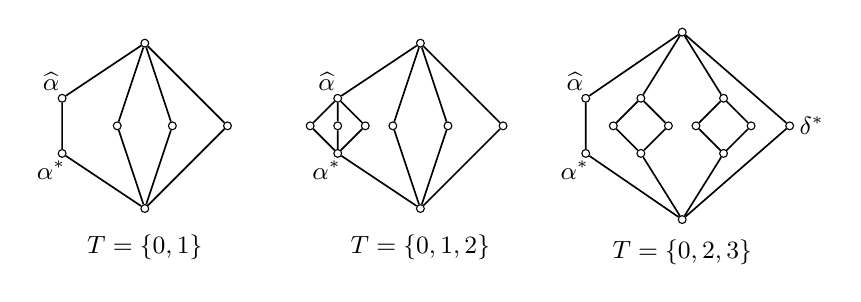
\begin{tikzpicture}[scale=.7]
      % T = \{0, 1\}
      \node (150) at (1.5,0)  [draw, circle, inner sep=1.0pt] {};
      \node (01) at (0,1)  [draw, circle, inner sep=1.0pt] {};
      \node (02) at (0,2)  [draw, circle, inner sep=1.0pt] {};
      \node (115) at (1,1.5)  [draw, circle, inner sep=1.0pt] {};
      \node (215) at (2,1.5)  [draw, circle, inner sep=1.0pt] {};
      \node (315) at (3,1.5)  [draw, circle, inner sep=1.0pt] {};
      \node (153) at (1.5,3)  [draw, circle, inner sep=1.0pt] {};
      \draw[semithick] 
      (150) to (01) to (02) to (153) to (115) to (150) to (215) to (153) to (315) to (150);
      \draw[font=\small] (1.5,-.7) node {$T = \{0,1\}$};
      \draw[font=\small] (-.2,.7) node {$\alpha^*$};
      \draw[font=\small] (-.2,2.3) node {$\widehat{\alpha}$};

      % T = \{0, 1, 2\}
      \node (650) at (6.5,0)  [draw, circle, inner sep=1.0pt] {};
      \node (51) at (5,1)  [draw, circle, inner sep=1.0pt] {};
      \node (52) at (5,2)  [draw, circle, inner sep=1.0pt] {};
      \node (4515) at (4.5,1.5)  [draw, circle, inner sep=1.0pt] {};
      \node (515) at (5,1.5)  [draw, circle, inner sep=1.0pt] {};
      \node (5515) at (5.5,1.5)  [draw, circle, inner sep=1.0pt] {};
      \node (615) at (6,1.5)  [draw, circle, inner sep=1.0pt] {};
      \node (715) at (7,1.5)  [draw, circle, inner sep=1.0pt] {};
      \node (815) at (8,1.5)  [draw, circle, inner sep=1.0pt] {};
      \node (653) at (6.5,3)  [draw, circle, inner sep=1.0pt] {};
      \draw[semithick] 
      (650) to (51) to (515) to (52) to (653) to (615) to (650) to (715) to (653) to
      (815) to (650)
      (51) to (4515) to (52) to (5515) to (51);
      \draw[font=\small] (6.5,-.7) node {$T = \{0,1,2\}$};
      \draw[font=\small] (4.8,.7) node {$\alpha^*$};
      \draw[font=\small] (4.8,2.3) node {$\widehat{\alpha}$};

      % T = \{0, 2, 3\}
      \node (bot) at (11.25,-.2)  [draw, circle, inner sep=1.0pt] {};
      \node (top) at (11.25,3.2)  [draw, circle, inner sep=1.0pt] {};
      \node (a) at (9.5,1)  [draw, circle, inner sep=1.0pt] {};
      \node (A) at (9.5,2)  [draw, circle, inner sep=1.0pt] {};
      \draw[font=\small] (9.3,.7) node {$\alpha^*$};
      \draw[font=\small] (9.3,2.3) node {$\widehat{\alpha}$};


      \node (b) at (10.5,1)  [draw, circle, inner sep=1.0pt] {};
      \node (b1) at (10,1.5)  [draw, circle, inner sep=1.0pt] {};
      \node (b2) at (11,1.5)  [draw, circle, inner sep=1.0pt] {};
      \node (B) at (10.5,2)  [draw, circle, inner sep=1.0pt] {};

      \node (c) at (12,1)  [draw, circle, inner sep=1.0pt] {};
      \node (c1) at (11.5,1.5)  [draw, circle, inner sep=1.0pt] {};
      \node (c2) at (12.5,1.5)  [draw, circle, inner sep=1.0pt] {};
      \node (C) at (12,2)  [draw, circle, inner sep=1.0pt] {};

      \node (d) at (13.2,1.5)  [draw, circle, inner sep=1.0pt] {};
      \draw[font=\small] (13.6,1.5) node {$\delta^*$};
      \draw[semithick] 
      (bot) to (a) to (A) to (top) to (B) to (b1) to (b) to (b2) to (B)
      (b) to (bot) to (c) to (c1) to (C) to (c2) to (c)
      (C) to (top) to (d) to (bot);
      \draw[font=\small] (11.25,-.8) node {$T = \{0, 2, 3\}$};

    \end{tikzpicture}

    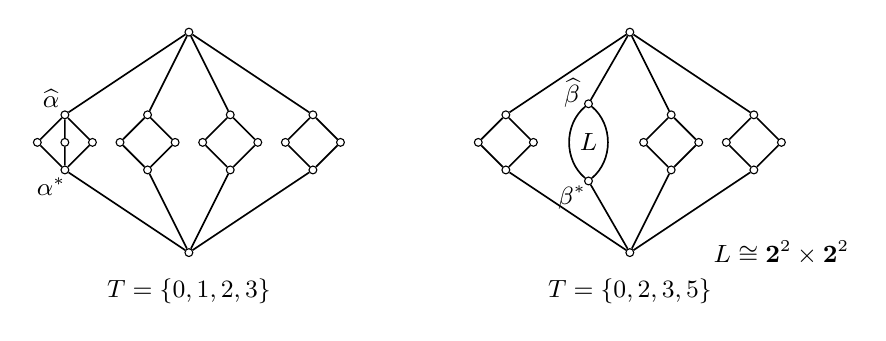
\begin{tikzpicture}[scale=.7]
      % T = \{0, 1, 2, 3\}
      \node (bot) at (3.25,0.5)  [draw, circle, inner sep=1.0pt] {};
      \node (top) at (3.25,4.5)  [draw, circle, inner sep=1.0pt] {};

      \node (a) at (1,2)  [draw, circle, inner sep=1.0pt] {};
      \node (a1) at (.5,2.5)  [draw, circle, inner sep=1.0pt] {};
      \node (a2) at (1,2.5)  [draw, circle, inner sep=1.0pt] {};
      \node (a3) at (1.5,2.5)  [draw, circle, inner sep=1.0pt] {};
      \node (A) at (1,3)  [draw, circle, inner sep=1.0pt] {};
      \draw[font=\small] (.75,1.7) node {$\alpha^*$};
      \draw[font=\small] (.75,3.3) node {$\widehat{\alpha}$};

      \node (b) at (2.5,2)  [draw, circle, inner sep=1.0pt] {};
      \node (b1) at (2,2.5)  [draw, circle, inner sep=1.0pt] {};
      \node (b2) at (3,2.5)  [draw, circle, inner sep=1.0pt] {};
      \node (B) at (2.5,3)  [draw, circle, inner sep=1.0pt] {};

      \node (c) at (4,2)  [draw, circle, inner sep=1.0pt] {};
      \node (c1) at (3.5,2.5)  [draw, circle, inner sep=1.0pt] {};
      \node (c2) at (4.5,2.5)  [draw, circle, inner sep=1.0pt] {};
      \node (C) at (4,3)  [draw, circle, inner sep=1.0pt] {};

      \node (d) at (5.5,2)  [draw, circle, inner sep=1.0pt] {};
      \node (d1) at (5,2.5)  [draw, circle, inner sep=1.0pt] {};
      \node (d2) at (6,2.5)  [draw, circle, inner sep=1.0pt] {};
      \node (D) at (5.5,3)  [draw, circle, inner sep=1.0pt] {};

      \draw[semithick] 
      (bot) to (a) to (a1) to (A) to (a2) to (a) to (a3) to (A) to (top) to 
      (B) to (b1) to (b) to (b2) to (B)
      (b) to (bot) to (c) to (c1) to (C) to (c2) to (c)
      (C) to (top) to (D) to (d1) to (d) to (d2) to (D)
      (d) to (bot);
      \draw[font=\small] (3.25,-.2) node {$T = \{0,1,2,3\}$};

      % T = \{0, 2, 3, 5\}
      \node (Rbot) at (11.25,0.5)  [draw, circle, inner sep=1.0pt] {};
      \node (Rtop) at (11.25,4.5)  [draw, circle, inner sep=1.0pt] {};

      \node (Ra) at (9,2)  [draw, circle, inner sep=1.0pt] {};
      \node (Ra1) at (8.5,2.5)  [draw, circle, inner sep=1.0pt] {};
      \node (Ra2) at (9.5,2.5)  [draw, circle, inner sep=1.0pt] {};
      \node (RA) at (9,3)  [draw, circle, inner sep=1.0pt] {};

      \node (Rb) at (10.5,1.8)  [draw, circle, inner sep=1.0pt] {};
      \node (RB) at (10.5,3.2)  [draw, circle, inner sep=1.0pt] {};
      \draw[font=\small] (10.2,1.5) node {$\beta^*$};
      \draw[font=\small] (10.2,3.4) node {$\widehat{\beta}$};

      \node (Rc) at (12,2)  [draw, circle, inner sep=1.0pt] {};
      \node (Rc1) at (11.5,2.5)  [draw, circle, inner sep=1.0pt] {};
      \node (Rc2) at (12.5,2.5)  [draw, circle, inner sep=1.0pt] {};
      \node (RC) at (12,3)  [draw, circle, inner sep=1.0pt] {};

      \node (Rd) at (13.5,2)  [draw, circle, inner sep=1.0pt] {};
      \node (Rd1) at (13,2.5)  [draw, circle, inner sep=1.0pt] {};
      \node (Rd2) at (14,2.5)  [draw, circle, inner sep=1.0pt] {};
      \node (RD) at (13.5,3)  [draw, circle, inner sep=1.0pt] {};

      \draw[semithick] 
      (Rbot) to (Ra) to (Ra1) to (RA) to (Ra2) to (Ra) 
      (RA) to (Rtop) to (RB)
      (Rb) to (Rbot) to (Rc) to (Rc1) to (RC) to (Rc2) to (Rc)
      (RC) to (Rtop) to (RD) to (Rd1) to (Rd) to (Rd2) to (RD)
      (Rd) to (Rbot);
      \draw [semithick]  
      (Rb) to [out=140,in=-140] (RB)
      (RB) to [out=-40,in=40] (Rb);
      \draw[font=\small] (10.5,2.5) node {$L$};

      \draw[font=\small] (11.25,-.2) node {$T = \{0,2,3, 5\}$};
      \draw[font=\small] (14,.5) node {$L\cong \two^2\times\two^2$};

    \end{tikzpicture}
\end{frame}
%% Since $\beta = | 0, 3 | 2, 5 | 1, 4 |$, when $T = \{0,2,3, 5\}$, the interval
%% $[\beta^*,\widehat{\beta}]$ is 
%% %$\Eq(2)^2 \times \Eq(2)^2  = \two^2\times\two^2$.  
%% $\two^2\times\two^2$.  
%% In Figure~\ref{fig:ConOverAlgebras2}, we denote this abstractly by $L$,
%% instead of drawing all 16 points of this interval.

%% \end{example}

%% Next, consider the situation depicted in the last congruence lattice of
%% Figure~\ref{fig:ConOverAlgebras2}, where 
%% $L \cong \two^2\times\two^2$, and
%% suppose we prefer that all the other $\resB$-inverse images be trivial:
%% $
%% [\beta^*,\widehat{\beta}]\cong \two^2\times\two^2; \,%\quad 
%% \alpha^*=\widehat{\alpha}; \, %\quad
%% \gamma^*=\widehat{\gamma};\,  %\quad
%% \delta^*=\widehat{\delta}.
%% $
%% In other words, we seek a finite algebraic
%% representation of the lattice in Figure~\ref{fig:ConOverAlgebras3}.
%% \begin{figure}[h!]
%%   \centering
%%     \begin{tikzpicture}[scale=.6]
%%       \node (Rbot) at (11.25,0.5)  [draw, circle, inner sep=1.0pt] {};
%%       \node (Rtop) at (11.25,4.5)  [draw, circle, inner sep=1.0pt] {};
%%       \node (Ra) at (9.25,2.5)  [draw, circle, inner sep=1.0pt] {};
%%       \node (Rb) at (10.75,1.8)  [draw, circle, inner sep=1.0pt] {};
%%       \node (RB) at (10.75,3.2)  [draw, circle, inner sep=1.0pt] {};
%%       \node (Rc) at (12,2.5)  [draw, circle, inner sep=1.0pt] {};
%%       \node (Rd) at (13.25,2.5)  [draw, circle, inner sep=1.0pt] {};
%%       \draw[semithick] 
%%       (Rbot) to (Ra) to (Rtop) to (RB)
%%       (Rb) to (Rbot) to (Rc) to (Rtop) to (Rd) to (Rbot);
%%       \draw [semithick]  
%%       (Rb) to [out=140,in=-140] (RB)
%%       (RB) to [out=-40,in=40] (Rb);
%%       \draw[font=\small] (10.75,2.5) node {$L$};
%%     \end{tikzpicture}
%%   \caption{A lattice which motivates further expansion of the set of basic 
%%     operations in the overalgebra.}
%%   \label{fig:ConOverAlgebras3}
%% \end{figure}
%% This is easy to achieve by adding more operations in the overalgebra
%% construction described above.
%% In fact, it is possible to introduce additional operations
%% so that, if $\beta = \Cg^\bB(x,y)$, then $\theta^* = \widehat{\theta}$ for all
%% $\theta \in \Con\bB$ with $\theta \ngeq \beta$. %%   \begin{itemize}
%%   \item put stuff here...
%%   \end{itemize}
%% \end{frame}

%% \begin{frame}[fragile,label=Extensions,shrink=5]{Generalizations...}
%%   \begin{itemize}
%%   \item put stuff here...
%%   \end{itemize}
%% \end{frame}

\begin{frame}[fragile,label=Limitations,shrink=5]{Limitations}

\vskip5mm

Two limitations of the foregoing construction:
\begin{enumerate}
\item The sizes $|T_r|$ of the partition lattice factors in 
\[
[\beta^*, \widehat{\beta}] \cong \prod_{r=1}^m (\Eq |T_r|)^{m-1}
\] 
are limited by the size of the blocks of $\beta$.

\vskip3mm

\item If $\beta$ is not principal, 
$[\theta^*, \htheta]$ may be non-trivial for some $\theta \ngeq \beta$.
\end{enumerate}
\end{frame}

\begin{frame}[fragile,label=OAextension2,shrink=5]{A Generalization}
 %% \begin{columns}
 %%  \begin{column}{0.8\textwidth}

\begin{theorem}
Let $\bB = \<B, F\>$ be a finite algebra. Suppose
\[
\beta = \Cg^{\bB}((a_1, b_1), \dots, (a_{K-1},b_{K-1}))
\]
has $m$ blocks and fix $N<\infty$.

\vskip3mm

There exists an overalgebra $\<A, F_A\>$
%Then, $\beta^* = \Cg^{\bA}(\beta)$ is given by
such that the interval $\beta\resB^{-1} \leq \Con \bA$ is 
%If $\beta$ has transversal $\{a_1, c_1, c_2, \dots, c_{m-1}\}$, then
%{\small \[ 
%% \beta^* = \bigcup_{j=0}^{MK} \beta^{\bB_j} \cup 
%% \left(\bigcup_{i=0}^{MK}t_i/\beta^{\bB_i}\right)^2, \quad
%%   \widehat{\beta} = \beta^* 
%% \cup 
%% \bigcup_{i=1}^{m-1}\left(\bigcup_{\ell \in \sE} c_i^\ell/\beta^{\bB_{\ell}}\right)^2
%% \cup 
%% \bigcup_{i=1}^{m-1}\left(\bigcup_{\ell \in \sO}
%% c_i^\ell/\beta^{\bB_{\ell}}\right)^2.
%% \]}
\[
[\beta^*, \widehat{\beta}] \cong (\Eq (N))^{m-1}.
\]
Moreover, we can arrange it so that $\theta^* = \widehat{\theta}$ for all $\theta \ngeq \beta$ in $\Con \bA$.
\end{theorem}

  %% \end{column}
  %% \begin{column}{0.2\textwidth}

%% \begin{align*}
%% B_0\cap B_1 &=\{a_1\}=\{a_1^{1}\},\\
%% B_1\cap B_2 &=\{b^1_1\}=\{a_2^{2}\},\\
%% B_2\cap B_3 &=\{b^2_2\}=\{a_3^{3}\},\\
%% \vdots\\
%% B_{K-2}\cap B_{K-1} &= \{b_{K-2}^{K-2}\}=\{a_{K-1}^{K-1}\},\\
%% B_{K-1}\cap B_K = B_K\cap B_{K+1}&=\{b^{K-1}_{K-1}\}=\{b^{K}_{K-1}\}=\{b^{K+1}_{K-1}\},\\
%% B_{K+1}\cap B_{K+2}&=\{a^{K+1}_{K-1}\} =\{b^{K+2}_{K-2}\},\\
%% B_{K+2}\cap B_{K+3}&=\{a^{K+2}_{K-2}\} =\{b^{K+3}_{K-3}\},\\
%% \vdots\\
%% B_{2K-2}\cap B_{2K-1} &= \{a_{2}^{2K-2}\}=\{b_{1}^{2K-1}\},\\
%% B_{2K-1}\cap B_{2K} = B_{2K}\cap  B_{2K+1}&=\{a^{2K-1}_{1}\}=\{a^{2K}_{1}\}=\{a^{2K+1}_{1}\},\\
%% B_{2K+1}\cap B_{2K+2}&=\{b^{2K+1}_{1}\} =\{b^{2K+2}_{2}\},\\
%% B_{2K+2}\cap B_{2K+3}&=\{b^{2K+2}_{2}\} =\{b^{2K+3}_{3}\},\\
%% \vdots\\
%% B_{MK-2}\cap B_{MK-1} &= \{b_{MK-2}^{K-2}\}=\{a_{MK-1}^{K-1}\},\\
%% B_{MK-1}\cap B_{MK}&=\{b^{MK-1}_{K-1}\}=\{b^{MK}_{K-1}\}.
%% \end{align*}
%% All other intersections are empty.
%%   \end{column}
%%  \end{columns}

\vskip3mm
\uncover<2->{
{\scalefont{.7}
  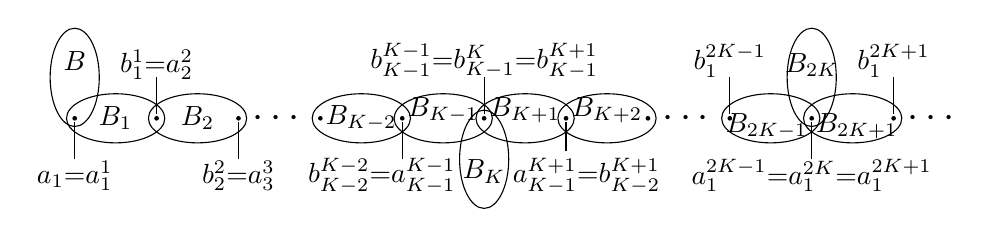
\begin{tikzpicture}[scale=.52]
    % B0
    \draw (0, 3.4) node {$B$};
    \draw (0,3) ellipse (.6cm and 1.2cm);

    % B1
    \draw (1,2) node {$B_1$};
    \draw (1,2) ellipse (1.2cm and .6cm);

    % B2
    \draw (3,2) node {$B_2$};
    \draw (3,2) ellipse (1.2cm and .6cm);

   \draw[font=\Large] (5, 2) node {$\cdots$};

    \draw (7,2) node {$B_{K-2}$};
    \draw (7,2) ellipse (1.2cm and .6cm);

    \draw (9,2.2) node {$B_{K-1}$};
    \draw (9,2) ellipse (1.2cm and .6cm);

    \draw (10,.7) node {$B_{K}$};
    \draw (10,1) ellipse (.6cm and 1.2cm);

    \draw (11,2.2) node {$B_{K+1}$};
    \draw (11,2) ellipse (1.2cm and .6cm);

    \draw (13,2.2) node {$B_{K+2}$};
    \draw (13,2) ellipse (1.2cm and .6cm);


   \draw[font=\Large] (15, 2) node {$\cdots$};

    \draw (16.9,1.8) node {$B_{2K-1}$};
    \draw (17,2) ellipse (1.2cm and .6cm);

    \draw (18,3.3) node {$B_{2K}$};
    \draw (18,3) ellipse (.6cm and 1.2cm);

    \draw (19.1,1.8) node {$B_{2K+1}$};
    \draw (19,2) ellipse (1.2cm and .6cm);

   \draw[font=\Large] (21, 2) node {$\cdots$};

   \node (1) at (0,2) [fill,circle,inner sep=.6pt] {};
   \draw (0, .6) node {$a_1{=}a_1^1$};
   \draw (0, 1) to  (0,1.9);

   \node (2) at (2,2) [fill,circle,inner sep=.6pt] {};
   \draw (2, 3.3) node {$b^1_1 {=} a^2_2$};
   \draw (2, 3) to  (2,2.1);

   \node (3) at (4,2) [fill,circle,inner sep=.6pt] {};
   \draw (4, .6) node {$b^2_2 {=} a^3_3$};
   \draw (4, 1) to  (4,1.9);

   \node (4) at (6,2) [fill,circle,inner sep=.6pt] {};
   \node (5) at (8,2) [fill,circle,inner sep=.6pt] {};
  \draw (7.5, .6) node {$b^{K-2}_{K-2} {=} a^{K-1}_{K-1}$};
   \draw (8, 1) to  (8,1.9);

   \node (6) at (10,2) [fill,circle,inner sep=.6pt] {};
   \draw (10, 3.4) node {$b^{K-1}_{K-1} {=} b^{K}_{K-1}{=} b^{K+1}_{K-1}$};
   \draw (10, 3) to  (10,2.1);

   \node (7) at (12,2) [fill,circle,inner sep=.6pt] {};
   \draw (12.5, .6) node {$a^{K+1}_{K-1} {=} b^{K+1}_{K-2}$};
   \draw (12, 1.2) to  (12,1.9);

   \node (8) at (14,2) [fill,circle,inner sep=.6pt] {};

   \node (9) at (16,2) [fill,circle,inner sep=.6pt] {};
   \draw (16, 3.4) node {$b^{2K-1}_{1}$};
   \draw (16, 3) to  (16,2.1);

   \node (10) at (18,2) [fill,circle,inner sep=.6pt] {};
   \draw (18, .6) node {$a^{2K-1}_{1} {=} a^{2K}_{1}{=} a^{2K+1}_{1}$};
   \draw (18, 1) to  (18,1.9);

   \node (11) at (20,2) [fill,circle,inner sep=.6pt] {};
   \draw (20, 3.4) node {$b^{2K+1}_{1}$};
   \draw (20, 3) to  (20,2.1);
   
  \end{tikzpicture}
}
}
\end{frame}


\begin{frame}[label=conclusion,shrink=5]{Seven element lattices: summary}
  \begin{columns}
    \begin{column}{0.2\textwidth}
      \begin{center}
        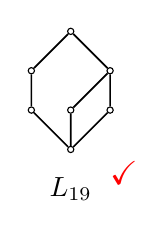
\begin{tikzpicture}[scale=.5]

          % L19
        \node (bottom) at (0,0)  [draw, circle, inner sep=\dotsize] {};
        \node (top) at (0,3)  [draw, circle, inner sep=\dotsize] {};
        \node (11) at (1,1)  [draw, circle, inner sep=\dotsize] {};
        \node (n11) at (-1,1)  [draw, circle, inner sep=\dotsize] {};
        \node (12) at (1,2)  [draw, circle, inner sep=\dotsize] {};
        \node (n12) at (-1,2)  [draw, circle, inner sep=\dotsize] {};
        \node (01) at (0,1)  [draw, circle, inner sep=\dotsize] {};

        \draw[semithick] (bottom) to (11) to (12) to (top) to (n12) to (n11) to (bottom) to (01) to (12);

          \draw (0,-1) node {$L_{19}$};
                {\color{red}\draw[font=\large] (1,-.6) node{$\text{\rlap{$\checkmark$}}$ };}
                %\draw[font=\footnotesize] (2.5,-.6) node { Jipsen};

        \end{tikzpicture}
      \end{center}
    \end{column}
    \begin{column}{0.2\textwidth}
      \begin{center}
        \begin{tikzpicture}[scale=.4]
          % L20
      \foreach \j in {0,...,4}
      {
        \node (0\j) at (0,\j)  [draw, circle, inner sep=\dotsize] {};
      }
      \node (152) at (1.5,2)  [draw, circle, inner sep=\dotsize] {};
      \node (n125) at (-1,2.5)  [draw, circle, inner sep=\dotsize] {};
      \draw[semithick] (01) to (02) to (03) to (04) to (n125) to (01) to (00) to (152) to (04);

          \draw (0,-1) node {$L_{20}$};
                {\color{red}\draw[font=\large] (1,-.6) node{$\text{\rlap{$\checkmark$}}$ };}
                %\draw[font=\footnotesize] (3,-.6) node { Jipsen};
        \end{tikzpicture}
      \end{center}
    \end{column}
  \end{columns}

  \begin{columns}
    \begin{column}{0.2\textwidth}
      \begin{center}
        \begin{tikzpicture}[scale=.4]

          
        \node (bottom) at (0,0)  [draw, circle, inner sep=\dotsize] {};
        \node (top) at (0,5)  [draw, circle, inner sep=\dotsize] {};
        \node (n115) at (-1,1.5)  [draw, circle, inner sep=\dotsize] {};
        \node (015) at (0,1.5)  [draw, circle, inner sep=\dotsize] {};
        \node (115) at (1,1.5)  [draw, circle, inner sep=\dotsize] {};
        \node (n252) at (-2.5,2)  [draw, circle, inner sep=\dotsize] {};
        \node (03) at (0,3)  [draw, circle, inner sep=\dotsize] {};
        \draw[semithick] 
        (bottom) to (n252) to (top)
        (bottom) to (n115) to (03) to (115) to
        (bottom) to (015) to (03) to (top);
       %\draw (-4.5,2.2) node {$L \cong$};



          \draw (0,-1) node {$L_{17}$};
                {\color{red}\draw[font=\large] (1,-1) node{$\text{\rlap{$\checkmark$}}$ };}

        \end{tikzpicture}
      \end{center}
    \end{column}

    \begin{column}{0.2\textwidth}
      \begin{center}
        \begin{tikzpicture}[scale=.5]

          %\newcommand{\dotsize}{1};
\node (0) at (0,0) [draw, circle,inner sep=\dotsize] {};
\node (1) at (-0,1) [draw, circle, inner sep=\dotsize] {};
\node (2) at (1,2) [draw, circle, inner sep=\dotsize] {};
\node (3) at (-1,2) [draw, circle, inner sep=\dotsize] {};
\node (4) at (-0,2) [draw, circle, inner sep=\dotsize] {};
\node (5) at (-0,3) [draw, circle, inner sep=\dotsize] {};
\node (6) at (-0,4) [draw, circle, inner sep=\dotsize] {};
%\draw[font=\scriptsize] (0,-.5) node {[A4, (C2 x C2 x C2 x C2) : A5]};
%\draw[font=\scriptsize] (0,-1) node {SmallGroup(960,11358) Index 80};

\draw[semithick]
(0) to (1)
(0) to (2)
(0) to (3)
(1) to (4)
(2) to (6)
(3) to (6)
(4) to (5)
(5) to (6);

          \draw (0,-.6) node {$L_{13}$};
                {\color{red}\draw[font=\large] (1,-.6) node{$\text{\rlap{$\checkmark$}}$ };}

        \end{tikzpicture}
      \end{center}
    \end{column}

    \begin{column}{0.2\textwidth}
      \begin{center}
        \begin{tikzpicture}[scale=.3]

          % L11 aka L3 
        \node (bottom) at (0,0)  [draw, circle, inner sep=\dotsize] {};
        \node (top) at (2,6)  [draw, circle, inner sep=\dotsize] {};
        \node (n22) at (-2,2)  [draw, circle, inner sep=\dotsize] {};
        \node (22) at (2,2)  [draw, circle, inner sep=\dotsize] {};
        \node (13) at (1,3)  [draw, circle, inner sep=\dotsize] {};
        \node (04) at (0,4)  [draw, circle, inner sep=\dotsize] {};
        \node (44) at (4,4)  [draw, circle, inner sep=\dotsize] {};

        \draw[semithick] (bottom) to (22) to (44) to (top) to (04) to (13) to (22)
        (bottom) to (n22) to (04);
  \draw (1,-1) node {$L_{11}$};
                {\color{red}\draw[font=\large] (2.3,-1) node { $\text{\rlap{$\checkmark$}}$};}

        \end{tikzpicture}
      \end{center}
    \end{column}

  \end{columns}


  \begin{columns}

    \begin{column}{0.2\textwidth}
      \begin{center}
        \begin{tikzpicture}[scale=.5]

          %% ``L9'' is the pentegon with two extra wings.
      \foreach \j in {0,3} 
      { \node (7\j) at (6.5,\j)  [draw, circle, inner sep=\dotsize] {};}
      \node (71) at (7,1.5)  [draw, circle, inner sep=\dotsize] {};
      \node (61) at (6,1.5)  [draw, circle, inner sep=\dotsize] {};
      \node (51) at (5,1.5)  [draw, circle, inner sep=\dotsize] {};
      \foreach \j in {1,2} 
      { \node (8\j) at (7.8,\j)  [draw, circle, inner sep=\dotsize] {};}
      \draw[semithick] (70) to (51) to (73) to (61) to (70) to (71) to (73) to
      (82) to (81) to (70);
      

          \draw (6.5,-1) node {$L_{9}$};
            {\color{red}\draw[font=\large] (7.5,-.6) node{$\text{\rlap{$\checkmark$}}$ };}
            %\draw[font=\large] (9.3,-.6) node { {\footnotesize Freese}};
        \end{tikzpicture}
      \end{center}
    \end{column}


    \begin{column}{0.2\textwidth}
      \begin{center}
        \begin{tikzpicture}[scale=.5]

          %%  The elusive winged-2x3 %%
      \node (01) at (0,1)  [draw, circle, inner sep=\dotsize] {};
      \foreach \j in {0,2} 
      { \node (1\j) at (1,\j)  [draw, circle, inner sep=\dotsize] {};}

      \foreach \j in {1,3} 
      { \node (2\j) at (2,\j)  [draw, circle, inner sep=\dotsize] {};}
      { \node (32) at (3,2)  [draw, circle, inner sep=\dotsize] {};}
      \draw[semithick] (10) to (01) to (12) to (23) to (32) to (21) to (10) (21) to (12);
      { \node (m11) at (-1,1)  [draw, circle, inner sep=\dotsize] {};}
      \draw[semithick] (10) to (m11) to (23);



          \visible<2>{\node (18) at (1,1.3)  [draw, circle, red, inner sep=25pt] {};}

          \draw (1,-.8) node {$L_7$};
        \end{tikzpicture}
      \end{center}
    \end{column}
  \end{columns}
\end{frame}

\frame[label=MO,shrink=5]{
  \frametitle{Has anyone seen this lattice?}
  \begin{center}
    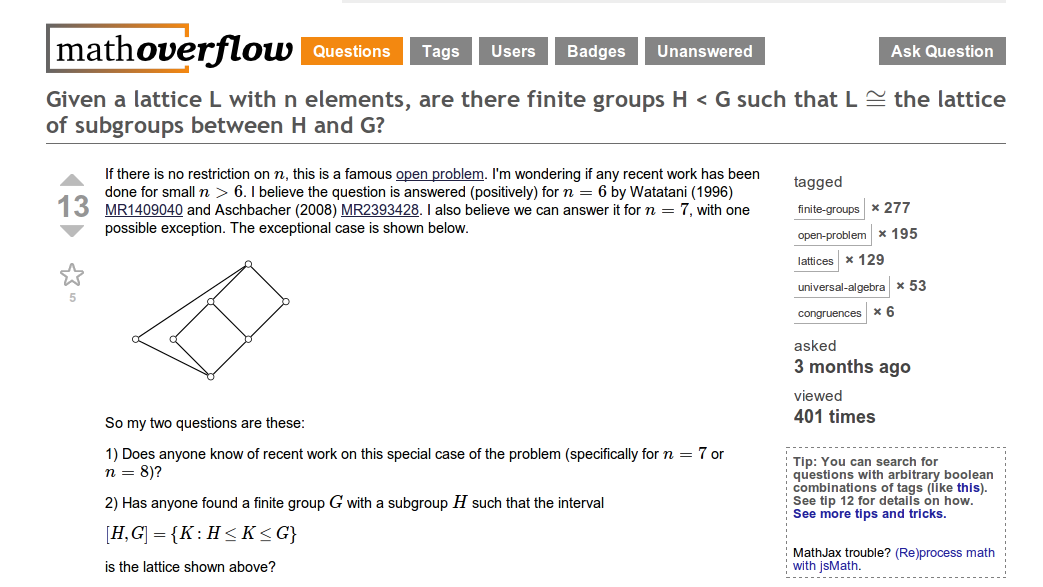
\includegraphics[height=2.8in]{MOquestion201204}
  \end{center}
}  

\begin{frame}[fragile,label=Conclusion,shrink=5]{The exceptional seven element lattice}
  \frametitle{Interval sublattice enforceable properties}
  \begin{columns}
    \begin{column}{0.7\textwidth}
      \begin{itemize}
      \item  $L_7$ cannot be obtained using the overalgebra construction.
        \vskip2mm
      \item<2-> A minimal representation of $L_7$ must come from a transitive $G$-set.
        \vskip2mm
      \item<3-> Suppose $L_7 \cong [H, G]$ for some finite groups $H<G$.\\[4pt]
        What can we say about the group $G$?
        \vskip2mm
      \item<4-> If we prove $G$ must have certain properties, then \FLRP\ has a
        positive answer iff every finite lattice is an interval
        in the subgroup lattice of a group \emph{satisfying all of these properties}.
        \note{
          \begin{itemize}
          \item Define $\core_G(H)$.  It is the largest normal subgroup in $G$
          contained in $H$.  It is also the kernel of the action of $G$ on the
          cosets of $H$.  
        \item $L_7 \cong [H, G]$, assume WLOG $H$ is \alert{core-free} in $G$.\\  
          Otherwise $L_7\cong [G/\core_G(H), H/\core_G(H)]$, and $H/\core_G(H)$ c.f. in $G/\core_G(H)$.
          \end{itemize}
        }
      \end{itemize}
    \end{column}
    \begin{column}{0.2\textwidth}
      \begin{center}
        \begin{tikzpicture}[scale=.5]
          %%  The elusive winged-2x3 %%
      \node (01) at (0,1)  [draw, circle, inner sep=\dotsize] {};
      \foreach \j in {0,2} 
      { \node (1\j) at (1,\j)  [draw, circle, inner sep=\dotsize] {};}

      \foreach \j in {1,3} 
      { \node (2\j) at (2,\j)  [draw, circle, inner sep=\dotsize] {};}
      { \node (32) at (3,2)  [draw, circle, inner sep=\dotsize] {};}
      \draw[semithick] (10) to (01) to (12) to (23) to (32) to (21) to (10) (21) to (12);
      { \node (m11) at (-1,1)  [draw, circle, inner sep=\dotsize] {};}
      \draw[semithick] (10) to (m11) to (23);


          \draw (1,-.8) node {$L_7$};
        \end{tikzpicture}
      \end{center}
    \end{column}
  \end{columns}

  \only<5->{
    \begin{theorem}
      \label{thm:except-seven-elem}
      Suppose $H<G$, \hskip2mm $\core_G(H) = 1$, \hskip2mm $L_7 \cong [H,G]$.
      \begin{enumerate}[(i)]
      \item<6-> $G$ is a primitive permutation group.
      \item<6-> If $N\ssubnormal G$, then $C_G(N) = 1$.
      \item<6-> $G$ contains no non-trivial abelian normal subgroup.
      \item<6-> $G$ is not solvable.
      \item<6-> $G$ is subdirectly irreducible.
      \item<6-> With the possible exception of at most one maximal subgroup, %, $M_1$ or $M_2$,
        all proper subgroups in the interval $[H,G]$ are core-free. 
      \end{enumerate}
    \end{theorem}
  }
  \note{  It is obvious that 
    \begin{itemize}
    \item (ii) $\Rightarrow$ (iii) $\Rightarrow$ (iv), and  
    \item (ii) $\Rightarrow$ (v), but we include these for
      emphasis;
    \item the hard work is in proving (ii) and (vi), but
      the main goal is the pair of restrictions (iii) and (v), which allow us to rule
      out a number of the O'Nan-Scott types describing primitive permutation
      groups. 
  \end{itemize}}
\end{frame}

%%% NEW STUFF %%%

\begin{frame}[fragile,label=SubgroupLattice]{Subgroup Lattice Basics}
Let $U$ and $H$ be subgroups of a finite group.
  \begin{itemize}
  \item<1-> By $UH$ we mean the \emph{set} $\{ u h \mid u\in U, h\in H\}$.\\[6pt]
  \item<2-> $U \join V = \<U,H\>$ means the group generated by $U$ and $H$.\\[6pt]
  \item<3-> $UH \subseteq \<U,H\>$ and 
    equality holds iff $U$ and $H$ permute: 
    \[
    UH = \<U,H\> \quad \Leftrightarrow \quad U H = H U.
    \]
  \end{itemize}
\visible<4->{
\begin{center}
  \begin{tikzpicture}[scale=.4]
    \node (H) at (4,4) [fill,circle,inner sep=\dotsize] {}; \draw (H) node [right] {$H$};
    \node (U) at (-4,4) [fill,circle,inner sep=\dotsize] {}; \draw (U) node [left] {$U$};
    \node (U0) at (0,0) [fill,circle,inner sep=\dotsize] {}; 
    \draw (1.5,-.75) node {$U_0 = U\cap H$};
    \node (UH) at (0,8) [fill,circle,inner sep=\dotsize] {}; \draw (UH) node [above] {$\<U,H\>$};
 \draw
    (U) to [out=-10,in=100] (U0) to [out=170,in=-80] (U)
    (UH) to [out=-10,in=100] (H) to [out=170,in=-80] (UH)
    (H) to [out=190,in=80] (U0) to [out=10,in=-100] (H)
    (UH) to [out=190,in=80] (U) to [out=10,in=-100] (UH);
    \visible<5->{\shade[top color=olivegreen,bottom color=gray!50] 
      (U) to [out=-10,in=100] (U0) to [out=170,in=-80] (U);
      \draw (-7,0) node {$[U_0,U]:=\{V \mid U_0 \leq V \leq U\}$};}
    \visible<6->{  \shade[top color=blue,bottom color=gray!50] 
      (UH) to [out=-10,in=100] (H) to [out=170,in=-80] (UH);
      \draw (7,6) node {$[H, \<U,H\>]$};}
    \visible<5->{ \node (V) at (-1.6,1.8) [fill,circle,inner sep=\dotsize] {};
      \draw (-2,2) node {$V$};}
    \end{tikzpicture}
\end{center}
}
\end{frame}

\begin{frame}[fragile,label=SubgroupLattice,shrink=5]{Interval Isomorphisms}
  \begin{columns}
    \begin{column}{0.3\textwidth}
      \begin{center}
        \begin{tikzpicture}[scale=.3]
              \node (H) at (4,4) [fill,circle,inner sep=\dotsize] {}; \draw (H) node [right] {$H$};
    \node (U) at (-4,4) [fill,circle,inner sep=\dotsize] {}; \draw (U) node [left] {$U$};
    \node (U0) at (0,0) [fill,circle,inner sep=\dotsize] {}; 
    \draw (1.5,-.75) node {$U_0 = U\cap H$};
    \node (UH) at (0,8) [fill,circle,inner sep=\dotsize] {}; \draw (UH) node
    [above] {$UH$};
 \draw
    (U) to [out=-10,in=100] (U0) to [out=170,in=-80] (U)
    (UH) to [out=-10,in=100] (H) to [out=170,in=-80] (UH)
    (H) to [out=190,in=80] (U0) to [out=10,in=-100] (H)
    (UH) to [out=190,in=80] (U) to [out=10,in=-100] (UH);

    \visible<2>{\shade[top color=olivegreen,bottom color=gray!-45] 
      (U) to [out=-10,in=100] (U0) to [out=170,in=-80] (U);}
    \visible<5->{
      \fill[color=olivegreen] 
      (U) to [out=-10,in=100] (U0) to [out=170,in=-80] (U);}
    \visible<2,5->{  \shade[top color=olivegreen,bottom color=gray!-45] 
      (UH) to [out=-10,in=100] (H) to [out=170,in=-80] (UH);}
    \visible<6->{\fill[color=orange]    
      (H) to [out=190,in=80] (U0) to [out=10,in=-100] (H);}
    \visible<6->{\shade[top color=orange,bottom color=gray!0]    
      (UH) to [out=190,in=80] (U) to [out=10,in=-100] (UH);}
       \end{tikzpicture}
      \end{center}
    \end{column}
    \begin{column}{0.7\textwidth}
      \begin{itemize}
      \item<1-> Assume $H\subnormal \<U, H\>$.
        \uncover<2->{
          \[
          \text{Then } \; UH = \<U, H\> \; \text{ and  } \; [U_0, U] \cong [H, UH].
          \]}
        \item<3-> Now drop assumption $H\subnormal \<U,H\>$,\\[4pt]
          assume $UH = \<U,H\>$, and define   
          \begin{equation*}
            %      \label{eq:dedekind-1}
            [U_0, U]^H := \{ V\in [U_0,U] \mid VH = HV\}.
          \end{equation*}
          the \alert{$H$-permuting subgroups}.
          \vskip2mm 
        \item<4-> If $U \subnormal UH$,
          define
          \begin{equation*}
            %  \label{eq:dedekind-2}
            [U_0, U]_H := \{ V\in [U_0,U] \mid H\leq N_{UH}(V)\}, 
          \end{equation*}
          the \alert{$H$-invariant subgroups}: 
          $h \, V \,h^{-1} = V$ for all $h\in H$.
      \end{itemize}
    \end{column}
  \end{columns}
\vskip-2mm

  \visible<5->{
%The main result relating these sets to $[H, UH]$ is
    % Lemma on H-invariant isomorphic intervals
    \begin{lemma}
      \label{lemma-wjd-4}
      \begin{enumerate}
      \item $[H, UH]  \cong  [U_0, U]^H \leq [U_0, U]$ \only<6>{ and \hskip2mm $[U, UH]
        \cong  [U_0, H]^U \leq [U_0, H]$}
\\[6pt]
      \item If $U \subnormal UH$, then  $[U_0, U]_H  = [U_0, U]^H \leq [U_0, U]$.\\[6pt]
      \item If $H \subnormal UH$,  then  $[U_0, U]_H  = [U_0, U]^H = [U_0, U]$.
      \end{enumerate}
    \end{lemma}
}
\note{
  \begin{itemize}
  \item 
  Since $G=UH$ is a group, the hypothesis of (ii) is equivalent to
$H\leq N_G(U)$, and the hypothesis of (iii) is equivalent to $U\leq N_G(H)$.
\item Part (i) of the lemma says that when two subgroups permute, we can
identify the interval above either one of them with the sublattice of
subgroups below the other that permute with the first.
\item Part (ii) is similar except we identify the interval above $H$ with
the  sublattice of $H$-invariant subgroups below $U$.
\item Once we have proved (i), the
proof of (iii) follows trivially from the Noether isomorphism theorem.
  \end{itemize}}

\end{frame}


\begin{frame}[fragile,label=Dedekind]{Dedekind's Rule}
The proof relies on the following modular law for subgroups:

\vskip3mm

\begin{theorem}[Dedekind's rule]
  \label{lemma-dedekind}
Let $A, B, C$ be subgroups of $G$ with $A\leq B$.  Then,
%% \begin{align*}
%% %\label{eq:dedekind1}
%% A(C\cap B) &= AC \cap B,\qquad \text{ and }\\
%% %\label{eq:dedekind2}
%% (C\cap B)A &= CA \cap B.
%% \end{align*}
\[
A(C\cap B) = AC \cap B \quad \text{ and }
\quad (C\cap B)A = CA \cap B.
\]
\end{theorem}

\vskip3mm

In other words, no pentagons.
\note{Draw picture of $N_5$ with $A\leq B$ to demonstrate that it contradicts Dedekind's rule.}
\end{frame}

\begin{frame}[fragile,label=ProofOfIntervalIsomorphism,shrink=5]{Proof of Interval Isomorphism Lemma}
  \begin{columns}
    \begin{column}{0.4\textwidth}
      {\bf Claim:} $[H, UH]  \cong  [U_0, U]^H \leq [U_0, U]$.

\vskip5mm

      \begin{center}
        \begin{tikzpicture}[scale=.3]
              \node (H) at (4,4) [fill,circle,inner sep=\dotsize] {}; \draw (H) node [right] {$H$};
    \node (U) at (-4,4) [fill,circle,inner sep=\dotsize] {}; \draw (U) node [left] {$U$};
    \node (U0) at (0,0) [fill,circle,inner sep=\dotsize] {}; 
    \draw (1.5,-.75) node {$U_0 = U\cap H$};
    \node (UH) at (0,8) [fill,circle,inner sep=\dotsize] {}; \draw (UH) node
    [above] {$UH$};
 \draw
    (U) to [out=-10,in=100] (U0) to [out=170,in=-80] (U)
    (UH) to [out=-10,in=100] (H) to [out=170,in=-80] (UH)
    (H) to [out=190,in=80] (U0) to [out=10,in=-100] (H)
    (UH) to [out=190,in=80] (U) to [out=10,in=-100] (UH);

          \fill[color=olivegreen] 
          (U) to [out=-10,in=100] (U0) to [out=170,in=-80] (U);
          \shade[top color=olivegreen,bottom color=gray!-45] 
          (UH) to [out=-10,in=100] (H) to [out=170,in=-80] (UH);
          \node (V) at (-2.3,2.5) [fill,circle,inner sep=\dotsize] {};
          \node (VH) at (1.7,6.5){};
          \draw (-2.7,2.9) node {$V$};
          \node (X) at (2.5,5.3) [fill,circle,inner sep=\dotsize] {};
          \node (UcapX) at (-1.5,1.3){};
          \draw (3,5.2) node {$X$};
          \draw[semithick,dotted] 
          (V) to [out=65,in=-155] (VH)
          (X) to [out=-155,in=65] (UcapX);
        \end{tikzpicture}
      \end{center}
    \end{column}
    \begin{column}{0.7\textwidth}
      \begin{itemize}
      \item<1-> 
        The following maps are inverse order isomorphisms:
        \begin{align*}
          \phi: \;& [H, UH] \ni X \mapsto U\cap X \in [U_0, U]^H\\[6pt]
          \psi: \;& [U_0, U]^H \ni V \mapsto VH \in [H, UH].
        \end{align*}
        \begin{itemize}
        \item<2-> Fix $X\in [H, UH]$.  By Dedekind's rule,
          \[
          (U\cap X) H = UH \cap X= HU \cap X = H(U \cap X),
          \]
          so $U\cap X \in [U_0, U]^H$.\\[6pt]
        \item<3->For $V\in [U_0, U]^H$, $VH = HV$ implies $VH \in [H, UH]$. \\[6pt]
        \item<4->  $\psi \circ \phi$ and 
          $\phi \circ \psi$ are the identity maps:
          \[
          \psi \circ \phi (X) = (U\cap X)H =UH \cap X = X,
          \]
          \[
          \phi \circ \psi(V)= VH \cap U =V(H\cap U)= V.
          \]
        \item<5->The maps are order preserving:
          \[X\leq Y \; \Rightarrow \; U\cap X \leq U\cap Y\]
          \[V\leq W \; \Rightarrow \; VH \leq WH.\]
          So, $\phi$ and $\psi$ are inverse order isomorphisms.
        \end{itemize}

      \item<6-> $[U_0, U]^H$ is a sublattice of $[U_0,U]$.

      \end{itemize}
    \end{column}
  \end{columns}
  %\vskip2mm

\end{frame}





\begin{frame}[fragile,label=L7second]{The Exceptional Seven Element Lattice}
  \begin{center}
    {\scalefont{.75}
      \begin{tikzpicture}[scale=.7]
              \node (J1) at (0,1)  [draw, circle, inner sep=\dotsize] {};
      \draw (.36, 1) node {$J_1$};
      \node (H) at (1,0)  [draw, circle, inner sep=\dotsize] {};
      \draw (1.16, -.2) node {$H$};
      \node (M2) at (1,2)  [draw, circle, inner sep=\dotsize] {};
      \draw (1.4, 2) node {$M_2$};
      \node (J2) at (2,1)  [draw, circle, inner sep=\dotsize] {};
      \draw (2.2, .8) node {$J_2$};
      \node (G) at (2,3)  [draw, circle, inner sep=\dotsize] {};
      \draw (2.3, 3.1) node {$G$};
      \node (M1) at (3,2)  [draw, circle, inner sep=\dotsize] {};
      \draw (3.35, 2) node {$M_1$};
      \node (K) at (-1,1.2)  [draw, circle, inner sep=\dotsize] {};
      \draw (-1.28, 1.15) node {$K$};

      \draw[semithick] (H) to (J1) to (M2) to (G) to (M1) to (J2) to (H) (J2) to (M2);
      \draw[semithick] (H) to (K) to (G);

      \end{tikzpicture}
    }
  \end{center}

\begin{theorem}
\label{thm:except-seven-elem}
Suppose $H<G$, $\core_G(H) = 1$, and 
$L_7 \cong [H,G]$.  Then
\begin{enumerate}[(i)]
\item<1-> $G$ is a primitive permutation group.
\item<1-> If $N\ssubnormal G$, then $C_G(N) = 1$.
\item<1-> $G$ contains no non-trivial abelian normal subgroup.
\item<1-> $G$ is not solvable.
\item<1-> $G$ is subdirectly irreducible.
\item<1-> With the possible exception of at most one maximal subgroup, $M_1$ or $M_2$,
  all proper subgroups in the interval $[H,G]$ are core-free. 

%% The three subgroups in $[H,G]$ which cover $H$ (the atoms) are
%%   core-free.  At least one two of the three maximal subgroups (the co-atoms) in
%%   the interval are core-free. 
\end{enumerate}
\end{theorem}
%% \note{  It is obvious that 
%%   \begin{itemize}
%%   \item (ii) $\Rightarrow$ (iii) $\Rightarrow$ (iv), and  
%% \item (ii) $\Rightarrow$ (v), but we include these for
%%   emphasis;
%% \item the hard work is in proving (ii) and (vi), but
%%   the main goal is the pair of restrictions (iii) and (v), which allow us to rule
%%   out a number of the O'Nan-Scott types describing primitive permutation
%%   groups. 
%%   \end{itemize}}
\end{frame}

\begin{frame}[fragile,label=IdeaOfL7Proof]{Idea of the proof}
    %% \begin{column}{0.3\textwidth}
      \begin{center}
        {\scalefont{.78}
          \begin{tikzpicture}[scale=1]
      \node (N) at (-.6,0)  [draw, circle, inner sep=1pt] {};
      \draw (-.9, 0) node {$N$};
      \node (NcapH) at (.2,-1)  [draw, circle, inner sep=1pt] {};
      \node (J1) at (0.2,1)  [draw, circle, inner sep=1pt] {};
      \draw (-.15, 1.05) node {$J_1$};
      \node (H) at (1,0)  [draw, circle, inner sep=1pt] {};
      \draw (1.16, -.2) node {$H$};
      \node (M2) at (1,2)  [draw, circle, inner sep=1pt] {};
      \draw (.6, 2.1) node {$M_2$};
      \node (J2) at (1.8,1)  [draw, circle, inner sep=1pt] {};
      \draw (1.35, 1.) node {$J_2$};
      \node (G) at (1.8,3)  [draw, circle, inner sep=1pt] {};
      \draw (2.1, 3.1) node {$G$};
      \node (M1) at (2.6,2)  [draw, circle, inner sep=1pt] {};
      \draw (2.1, 2) node {$M_1$};
      \node (K) at (3.5,1.8)  [draw, circle, inner sep=1pt] {};
      \draw (3.85, 1.8) node {$K$};
      \draw[semithick,dotted] (J1) to (N) to (NcapH) to (H);
      \visible<4->{\draw[very thick] (J1) to (M2) to (G) (H) to (K);}
      \draw[semithick] (J1) to (M2) to (G) (H) to (K);
      \draw[semithick] (H) to (J1) to (M2) to (G) to (M1) to (J2) to (H) to (K)
      to (G) (J2) to (M2);
    \end{tikzpicture}
 }
\end{center}
      
  %%   \end{column}
  %% \end{columns}

  %% \begin{columns}
  %%   \begin{column}{0.7\textwidth}
      {\bf Claim:} 
      $J_1$ and $J_2$ are core-free subgroups of $G$.\\[6pt]
      {\bf Proof:}
      \begin{itemize}
      \item<2->
      If $N\ssubnormal G$ then $NH$ permutes with each subgroup containing $H$.  
      \note{Let $H \leq X \leq G$.  Then $NHX = NX = XN= XHN = XNH$.}
      \item<3-> If $1\neq N\leq J_1$, then $NH = J_1$, so $J_1$ and $K$ permute.
      \item<4-> Since $J_1K = G$ and $J_1\cap K = H$, our lemma yields
      \[
        [J_1, G] \cong [H, K]^{J_1} = \{X \in[H, K] \mid J_1X=XJ_1 \}.
        \]
   \uncover<5->{Impossible!}
      \end{itemize}

    %% \end{column}


\end{frame}

\begin{frame}[fragile,label=OSTheorem]{Achbacher-O'Nan-Scott Theorem}
Let $G$ be a primitive permutation
group of degree $d$, and let $N := \Soc(G) \cong T^m$ with $m \geq 1$. 
Then one of the following holds.
\vskip2mm
\begin{enumerate}
\item 
$N$ is regular and
  \begin{itemize}
  \item 
  \alert{Affine type} $T$ is cyclic of order $p$, so $|N| = p^m$ . Then 
$d = p^m$ and $G$ is permutation isomorphic to a subgroup of the affine
general linear group $\AGL(m,p)$.
\vskip2mm
\item \alert{Twisted wreath product type} $m \geq 6$, the group $T$ is 
  nonabelian and $G$ is a group of \emph{twisted wreath product type}, with
  $d = |T|^m$.
  \end{itemize}
\vskip2mm
\item $N$ is non-regular, non-abelian, and
  \begin{itemize}
  \item 
\alert{Almost simple} $m = 1$ and $T \leq G \leq \Aut(T)$.
\vskip2mm
\item \alert{Product action} $m \geq 2$ and $G$ is permutation isomorphic to a
subgroup of the product action wreath product $P \wr S_{m/l}$ of degree
$d = nm/l$. The group $P$ is primitive of type 2.(a) or 2.(c), $P$ has
degree $n$ and $\Soc(P) \cong T^l$, where $l \geq 1$ divides $m$.
\vskip2mm
\item 
\alert{Diagonal type} $m \geq 2$ and $T^m \leq G \leq T^m . (\Out(T ) \times S_m)$, with
the diagonal action. The degree $d = |T|^{m-1}$.
  \end{itemize}
\end{enumerate}
\end{frame}

\setbeamercovered{invisible}

\begin{frame}[fragile,label=FinalConclusions]{Conclusions}
  \begin{itemize}
  \item<1-5> We have new methods for building new finite algebras out of
    old so that the congruence lattice changes in predictable ways.
\vskip2mm
  \item<2-5> Using these and other methods we have found representations for all
    finite lattices with at most 7 elements with one exception, thus
    idetifying the unique smallest lattice for which there's no known
    representation. 
\vskip2mm
  \item<3-5> We developed techniques for putting restrictions on groups that
    have certain lattices as intervals in their subgroup lattices.
\vskip2mm
\item<4-5> By studying the lattice $L_7$, we can restrict the class of
  groups which could possibly represent this lattice.  (We believe a slightly
  modified versoin of this lattice will restrict to the class of almost simple
  groups.)
\vskip2mm
\item<5-5> Future work: Restrict to almost simple groups and then solve the problem using the CFSG Theorem.
  \end{itemize}
  %% \vskip5mm 
  %% \visible<4>{
  %%   \hskip-5mm          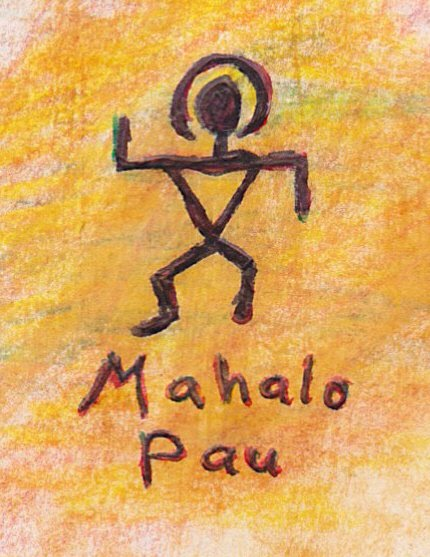
\includegraphics[height=2in]{MahaloPau}
  %% }
\end{frame}
\begin{frame}[fragile,label=FinalConclusions]{}
  \begin{center}
  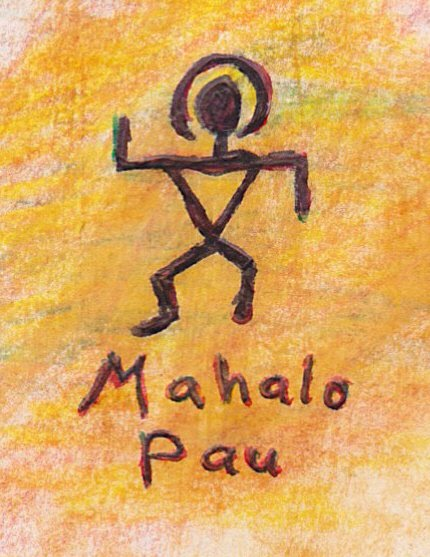
\includegraphics[height=2in]{MahaloPau}
  \end{center}
\end{frame}


\end{document}



%%%%%%%%%%%%% END DOCUMENT %%%%%%%%%%%%%%%%



Notice that to even
define $[U_0, U]_H$ we must have $H\leq N_G(U)$, and in this case, as we will
see below, the two sublattices coincide: 
$[U_0, U]_H  =  [U_0, U]^H$.  

We are finally ready to state the main result relating the sets defined
in~(\ref{eq:dedekind1}) and (\ref{eq:dedekind2}) (when they
exist) to the interval $[H, UH]$.
% Lemma on H-invariant isomorphic intervals
\begin{lemma}
  \label{lemma-wjd-4}
Suppose $U$ and $H$ are permuting subgroups of a group. %, that is, suppose $UH$ is a group.
Let $U_0 := U\cap H$.  Then
\begin{enumerate}[(i)]
\item $[H, UH]  \cong  [U_0, U]^H \leq [U_0, U]$.
\item If $U \subnormal UH$, then  $[U_0, U]_H  = [U_0, U]^H \leq [U_0, U]$.
\item If $H \subnormal UH$,  then  $[U_0, U]_H  = [U_0, U]^H = [U_0, U]$.
\end{enumerate}
\end{lemma}
\begin{remarks}
Since $G=UH$ is a group, the hypothesis of (ii) is equivalent to
$H\leq N_G(U)$, and the hypothesis of (iii) is equivalent to $U\leq N_G(H)$.
Part (i) of the lemma says that when two subgroups permute, we can
identify the interval above either one of them with the sublattice of
subgroups below the other that permute with the first.
Part (ii) is similar except we identify the interval above $H$ with
the  sublattice of $H$-invariant subgroups below $U$.  Once we have proved (i), the
proof of (iii) follows trivially from the Noether isomorphism theorem for
groups (\S~\ref{thm:Noether}), so we omit the details.
\end{remarks}

\begin{proof}
%% If $UH$ is a group, then the interval 
%% $[H, UH]$ is isomorphic to $[U_0, U]^H$.  
To prove (i), we show that the following maps are inverse order isomorphisms:
\begin{align}
\label{eq:inverse-isos}
\phi: \;& [H, UH] \ni X \mapsto U\cap X \in [U_0, U]^H\\
\psi: \;& [U_0, U]^H \ni V \mapsto VH \in [H, UH].\nonumber
\end{align}
Then we show that $[U_0, U]^H$ is a sublattice of $[U_0,U]$, that is, 
$[U_0, U]^H\leq [U_0,U]$.




















\begin{frame}[fragile,label=freeseOLD,shrink=5]{Construction of an algebra $\bA$ with $\Con \bA \cong L_9$.}

  \begin{columns}
    \begin{column}{0.2\textwidth}

      \centering
      \begin{tikzpicture}[scale=.7]
                \node (250) at (2.5,0)  [draw, circle, inner sep=\dotsize] {};
        \node (253) at (2.5,3)  [draw, circle, inner sep=\dotsize] {};
        \foreach \i in {1,...,4} 
                 { 
                   \node (\i15) at (\i,1.5)  [draw, circle, inner sep=\dotsize] {};
                   \draw[semithick] (250) to (\i15) to (253);
                 }

        \uncover<2->{
          \draw[font=\footnotesize] 
          (0.7,1.5) node {$\alpha$} (1.7,1.5) node {$\beta$}
          (3.3,1.5) node {$\gamma$} (4.3,1.5) node {$\delta$}
          (2.8,3.15) node {$1_B$} (2.83,-.15) node {$0_B$};
        }
        \visible<1>{
          \draw  (1,0) node {$M_4$};}
        \visible<2->{
          \draw  (1,0) node {$\Con \bB$};}
      \end{tikzpicture}
    \end{column}
    \begin{column}{0.8\textwidth}
      \begin{enumerate}[Step 1]
      \item<2-> 
        Take a permutational algebra $\bB = \<B, F\>$ with congruence lattice $\Con\bB \cong M_4$.

        \vskip6pt
        
        \note{There are infinitely many, but apart from those involving 
          $S_3$, $C_3 \times C_3$, and $(C_3 \times C_3) \rtimes C_3$, they are quite
          large.  The next smallest G-set with $M_4$ congruence lattice that we
          know of comes from the group 
          $G = [ ( (C_3 \times C_3) \rtimes C_2 ) \times ( (C_3 \times C_3) \rtimes C_2 ) ] \rtimes C_2$
          acting on right cosets of $H \cong D_8$.  The index in this case is $|G:H| = 81$.
          (In \GAP, {\tt G:=SmallGroup(648,725)}.)}

        {\small
          \onslide<4->{\underline{Example:}}
          \vskip4pt
%          \begin{itemize}
          \begin{itemize}[label=$\cdot$]
          \item<4->
            Let $B = \{0, 1, \dots, 5\}$ index the elements of $S_3$ and
            consider the right regular action of $S_3$ on itself.
            \vskip5pt
          \item<4->
            $g_0 = (0,4)(1,3)(2,5)$ and $g_1 = (0,1,2)(3,4,5)$ generate this
            action group, the image of $S_3 \hookrightarrow S_6$.
            \vskip5pt
          \item<4-> $\Con \<B , \{g_0, g_1\}\> \cong M_4$ with congruences
\vskip1pt
\[
\hskip-3mm            \alpha = | 0 1 2 | 3 4 5|, \; \beta = | 0 3 | 1 4 | 2 5 |, 
            \gamma = | 0 4|1 5| 2 3| , \; \delta = | 0 5|1 3| 2 4| .
            \]
          \end{itemize}
        }
      \end{enumerate}


    \end{column}
  \end{columns}

  \vskip-2mm

  \begin{columns}

    \begin{column}{0.2\textwidth}
      \begin{center}
        \begin{tikzpicture}[scale=.7]

                \node (70) at (6.5,0)  [draw, circle, inner sep=\dotsize] {};
      \node (71) at (7,1.5)  [draw, circle, inner sep=\dotsize] {};
      \node (73) at (6.5,3)  [draw, circle, inner sep=\dotsize] {};
      \node (61) at (6,1.5)  [draw, circle, inner sep=\dotsize] {};
      \node (51) at (5,1)  [draw, circle, inner sep=\dotsize] {};
      \node (52) at (5,2)  [draw, circle, inner sep=\dotsize] {};
      \node (81) at (8,1.5)  [draw, circle, inner sep=\dotsize] {};
      \draw[semithick] 
      (70) to (51) to (52) to (73)
      (70) to (61) to (73) 
      (70) to (71) to (73) 
      (70) to (81) to (73);

          \visible<1,2>{\draw  (5,0) node {$L_{9}$};}
          \visible<3->{\draw  (5,0) node {$\Con \bA$};}
          \visible<3->{\draw[font=\footnotesize] (4.7,2) node {$\widehat{\alpha}$} (4.7,1) node {$\alpha^*$};}

        \end{tikzpicture}
      \end{center}
    \end{column}
    \begin{column}{0.75\textwidth}

      \begin{itemize}
      \item<3-> {\rmfamily \emph{Goal: expand $\bB$ to an algebra $\bA$ that has
          $\alpha$ ``doubled'' in $\Con\bA$.}}
        \vskip4pt
%            {\small
              \onslide<5->{\underline{Example:}\hskip8pt $\alpha = \Cg^\bB(0,2)$. }
              \vskip4pt
%              \begin{itemize}[label=$*$]
%                \begin{enumerate}
            \item<5->[Step 2] Let $A = B_0 \cup B_1 \cup B_2$ where
              \vskip-6pt
              \begin{align*}
                B_0 &= \{ {\color<5>{blue}0}, 1, {\color<5>{green}2}, 3, 4, 5\} = B\\
                B_1 &= \{{\color<5>{blue}0}, 6, 7, 8, 9, 10\}\\
                B_2 &= \{ 11, 12, {\color<5>{green}2}, 13, 14, 15\}.
              \end{align*}
            \item<5->[Step 3] Define unary operations $e_0, e_1, e_2,\, s, \,g_0 e_0$, and $g_1 e_0$.
%                \end{enumerate}
%              \end{itemize}
%            }
      \end{itemize}
    \end{column}

  \end{columns}

\end{frame}


















\begin{frame}[fragile,label=OAopOLD,shrink=5]{Why does it work?}

  \begin{columns}
    \begin{column}{0.3\textwidth}
      \begin{center}
        $\Con \< B,\{g_0, g_1\}\>$

        \vskip-2pt
        \begin{align*}
          \alpha &= |0, 1, 2 | 3, 4, 5|\\[4pt]
          \beta &= |0, 3 | 1, 4 |2, 5 | \\[3pt]
          \gamma &= |0, 4| 1, 5|2, 3| \\[3pt]
          \delta &= |0, 5|1, 3|2, 4| 
        \end{align*}
      \end{center}
    \end{column}

    \begin{column}{0.3\textwidth}
      \begin{tikzpicture}[scale=.7]

        %% B0 %%
        \visible<1-13>{
          \foreach \j in {0,1,2} {
            \draw (\j -1, 0.5) node {$\j$};
            \pgfmathtruncatemacro{\x}{\j+3}
            \draw (\j -1, -0.5) node {$\x$};
          }
          \draw (0,-1.5) node {$B_0$};
          \draw[rounded corners,dotted] (-1.5,-1) rectangle (1.5,1);
        }
        \visible<12->{\draw (-1, 0.5) node {$0$};}

        %% B1 %%
        \foreach \j in {0,1,2} {
          \pgfmathtruncatemacro{\x}{10-\j}
          \draw (\j -3, 1.5) node {$\x$};
        }
        \draw (-3, .5) node {$7$} (-2, .5) node {$6$}; 
        \draw[rounded corners,blue] (-3.5,0) rectangle (-0.5,2);
        \draw  (-2,2.5) node {$B_1$};

        %% B2 %%
        \visible<1>{ 
          \foreach \j in {0,1,2} {
            \pgfmathtruncatemacro{\y}{15-\j}
            \draw (\j +1, 1.5) node {$\y$};
          }
          \draw (3, .5) node {$11$} (2, .5) node {$12$};
          \draw  (2,2.5) node {$B_2$};
          \draw[rounded corners,dotted] (3.5,0) rectangle (0.5,2);
        }

        %% Rotate B2 onto B0 %%
        \foreach \i in {0,1,...,11}{   
          \pgfmathtruncatemacro{\v}{\i+1}
          \visible<\v>{ 
            {\color<11-12>{gray}
              \eImageOfBTwo{\i} 
            }
          }
        }

        %% Rotate B0 onto B1 %%
        \foreach \i in {0,1,...,11}{
          \pgfmathtruncatemacro{\v}{\i+13}
          \visible<\v>{ 
            {\color<22-24>{gray}
              \eImageOfBZero{\i}       %% use -\i for clockwise rotation
            }
          }
        }

      \end{tikzpicture}
    \end{column}
  \end{columns}
  \begin{columns}
    \begin{column}{0.3\textwidth}
      \begin{itemize}
      \item $A = B_0 \cup B_1 \cup B_2$
        \vskip4pt
      \item Unary operations 
        \begin{align*}
          {\color{gray} e_0} & {\color{gray} : A \twoheadrightarrow B_0 } \\
          {\color{blue} e_1} &{\color{blue} : A \twoheadrightarrow B_1}\\
          {\color{gray} e_2} &{\color{gray} : A \twoheadrightarrow B_2}\\
          {\color{gray} s} &{\color{gray} : A \twoheadrightarrow B_0}
        \end{align*}
        \[
          {\color{gray} g e_0} {\color{gray} : A \stackrel{e_0}{\twoheadrightarrow} B_0 \stackrel{g}{\rightarrow} B_0}
          \]
      \end{itemize}
    \end{column}
    \begin{column}{0.5\textwidth}
      \begin{tikzpicture}[scale=.7]

        %%% B_0 %%%
        \draw (-1,0) node {$B_0 = \{$};
        \foreach \i in { 0, 1, 2, 3, 4, 5}{ 
          \draw (\i,0) node {$\i$}; 
          \visible<14-16,19-21,24-26>{ \draw [|->] (\i,0.5) -- (\i,1.1) ; }
          \visible<2-4,7-9,12>{ \draw [|->] (\i,-1.1) -- (\i,-0.5); }
        }
        \draw (5.5,0) node {$\}$};

        %%% B_1 %%%
        \draw (-1,1.5) node {$B_1 =\{$} (0,1.5) node {$0$};
        \foreach \i in { 6, 7, 8, 9, 10}{ \draw (\i-5,1.5) node {$\i$}; }
        \draw (5.5,1.5) node {$\}$};
        
        %%% B_2 %%%
        \draw (-1,-1.5) node {$B_2 =\{$} (0,-1.5) node {$11$} (1,-1.5) node {$12$} (2,-1.5) node {$2$};
        \foreach \i in { 13, 14, 15}{ \draw (\i-10,-1.5) node {$\i$}; }
        \draw (5.5,-1.5) node {$\}$};


      \end{tikzpicture}
    \end{column}

  \end{columns}
\end{frame}


















\begin{frame}[fragile,label=OAop4,shrink=5]{Why does it work?}

  \begin{columns}
    \begin{column}{0.3\textwidth}
      \begin{center}
        $\Con \< B,\{g_0, g_1\}\>$

        \vskip-2pt
        \begin{align*}
          \alpha &= |0, 1, 2 | 3, 4, 5|\\[4pt]
          \beta &= |0, 3 | 1, 4 |2, 5 | \\[3pt]
          \gamma &= |0, 4| 1, 5|2, 3| \\[3pt]
          \delta &= |0, 5|1, 3|2, 4| 
        \end{align*}
      \end{center}
    \end{column}

    \begin{column}{0.3\textwidth}
      \begin{tikzpicture}[scale=.7]

        %% B0 %%
        \foreach \j in {0,1,2} {
          \draw (\j -1, 0.5) node {$\j$};
          \pgfmathtruncatemacro{\x}{\j+3}
          \draw (\j -1, -0.5) node {$\x$};
        }
        \draw (0,-1.5) node {$B_0$};
        \draw[rounded corners,dotted] (-1.5,-1) rectangle (1.5,1);

        %% B1 %%
        \foreach \j in {0,1,2} {
          \pgfmathtruncatemacro{\x}{10-\j}
          \draw (\j -3, 1.5) node {$\x$};
        }
        \draw (-3, .5) node {$7$} (-2, .5) node {$6$}; 
        \draw[rounded corners,dotted] (-3.5,0) rectangle (-0.5,2);
        \draw  (-2,2.5) node {$B_1$};

        %% B2 %%
        \foreach \j in {0,1,2} {
          \pgfmathtruncatemacro{\y}{15-\j}
          \draw (\j +1, 1.5) node {$\y$};
        }
        \draw (3, .5) node {$11$} (2, .5) node {$12$};
        \draw  (2,2.5) node {$B_2$};
        \draw[rounded corners,dotted] (3.5,0) rectangle (0.5,2);


      \end{tikzpicture}
    \end{column}
  \end{columns}
  \begin{columns}
    \begin{column}{0.3\textwidth}
      \begin{itemize}
      \item $A = B_0 \cup B_1 \cup B_2$
        \vskip4pt
      \item Unary operations 
        \begin{align*}
          {\color{gray} e_0} & {\color{gray} : A \twoheadrightarrow B_0 } \\
          {\color{gray} e_1} &{\color{gray} : A \twoheadrightarrow B_1}\\
          {\color{gray} e_2} &{\color{gray} : A \twoheadrightarrow B_2}\\
          {\color{gray} s} &{\color{gray} : A \twoheadrightarrow B_0}
        \end{align*}
        \[
          {\color{blue} g e_0} {\color{blue} : A \stackrel{e_0}{\twoheadrightarrow} B_0 \stackrel{g}{\rightarrow} B_0}
          \]
      \end{itemize}
    \end{column}
    \begin{column}{0.5\textwidth}
      \begin{tikzpicture}[scale=.7]

        %%% B_0 %%%
        \draw (-1,0) node {$B_0 = \{$};
        \foreach \i in { 0, 1, 2, 3, 4, 5}{ 
          \draw (\i,0) node {$\i$}; 
        }
        \draw (5.5,0) node {$\}$};

        %%% B_1 %%%
        \draw (-1,1.5) node {$B_1 =\{$} (0,1.5) node {$0$};
        \foreach \i in { 6, 7, 8, 9, 10}{ \draw (\i-5,1.5) node {$\i$}; }
        \draw (5.5,1.5) node {$\}$};
        
        %%% B_2 %%%
        \draw (-1,-1.5) node {$B_2 =\{$} (0,-1.5) node {$11$} (1,-1.5) node {$12$} (2,-1.5) node {$2$};
        \foreach \i in { 13, 14, 15}{ \draw (\i-10,-1.5) node {$\i$}; }
        \draw (5.5,-1.5) node {$\}$};


      \end{tikzpicture}
    \end{column}

  \end{columns}
\end{frame}

